\documentclass[11pt]{article}
\usepackage[margin=1in]{geometry}
\usepackage{amsmath,amssymb}
\usepackage{graphicx}
\usepackage{booktabs}
\usepackage{float}
\usepackage{array}
\usepackage[hidelinks]{hyperref}
\usepackage{parskip}
\title{Certify What You Measure, Govern What You Cannot: A Range--Null Account of Accountability and Governed Detail Across Undersampled Imaging Operators}
\author{}\date{}
\begin{document}
\maketitle

\textit{Author placeholder --- Author One, Author Two, Author Three. Affiliation placeholder. Corresponding author: [email placeholder].}

\medskip\hrule\medskip

\section*{Abstract}

In low-rate compressive imaging --- single-pixel and ghost imaging, accelerated MRI, snapshot spectral imaging --- measurement consistency is not evidence of image correctness, and when the ground truth is unknown a learned reconstruction's fidelity cannot be assessed from its record alone. The reason is geometric: the record constrains only the measurement-visible row-space coordinate --- $P_R x = A^\dagger y$ in the noiseless model, its noisy counterpart $A^\dagger y = P_R x + A^\dagger\varepsilon$ otherwise --- while $P_0 x \in \ker A$ is invisible to the sensor, since $A P_0 = 0$. We turn this fact into an accountability framework and validate it on three explicit operators: a simulated single-pixel ghost-imaging matrix, the real masked-Fourier operator of NYU fastMRI single-coil knee $k$-space, and the real released CASSI coded aperture. First, we construct feasible-but-wrong witnesses --- two different scenes sharing one undersampled record, matched tighter than the noisy truth itself (to $\sim\!10^{-16}$). Second, we give a ground-truth-free, per-mode record-consistency audit that contracts the $i$-th measured residual mode by exactly $\lambda/(\lambda+\sigma_i^2)$; CASSI's non-uniform singular spectrum (a $528\times$ range) makes this contraction vary over $2\times10^4\times$ where masked-Fourier MRI's flat spectrum collapses to a single value. Third, a third-party forensic ledger decomposes published gains through each operator's own projectors: $91$--$92\%$ of the official fastMRI U-Net's PSNR gain and $93$--$101\%$ of thirteen published CASSI models' gains are null-supplied, not measured. The same boundary becomes a governance dial --- prior detail is injected only through $P_0$, so a null-space edit alters fine detail while $A\hat{x}_B = y$ holds to machine precision for every setting $B$ (locked GI: LPIPS $-32.6\%$ at $-0.45$ dB). The result is a two-ledger account: certify what the sensor measured; label and govern what the prior supplied. Scope is honest --- simulation and declared-operator level throughout.

\medskip\hrule\medskip

\section*{1. Introduction}

At 5\% sampling, a $64\times64$ ghost-imaging system records 205 bucket values for a 4096-pixel scene. The unmeasured 3891 degrees of freedom are not merely difficult to recover; they are invisible to the measurement operator. A learned reconstructor can therefore produce a sharp, natural-looking image, reproduce every recorded bucket, and still invent most of the visible detail. This paper asks how such a reconstruction should be audited: what did the bucket actually certify, and what did the prior merely supply?

The cause is one identity. With $A^\dagger$ the pseudoinverse and $P_R = A^\dagger A$, $P_0 = I - A^\dagger A$ the projectors onto the row space and null space of $A$,

$$A P_0 = 0,$$

so the noiseless record $Ax$ is a function of $P_R x$ alone, and a noisy record fixes only the noisy row-space coordinate $A^\dagger y = P_R x + A^\dagger\varepsilon$. In both cases two images that agree on the measured component produce the identical record no matter how much they differ elsewhere. Every quality metric integrates both components; the measurement sees one. Image quality and measurement accountability are therefore different quantities, and a pipeline can score well on the first while saying nothing about the second.

The paper has one geometry and three consequences. Because $A P_0 = 0$, the bucket cannot distinguish images that share a row-space component; we make this failure concrete with feasible-but-wrong witnesses that match a target's noisy record around $10^{-15}$ --- more tightly than the clean truth matches that same record (§2). The same geometry gives a positive result: the measured modes can be audited exactly, with a known contraction factor per mode, after any reconstructor (§3). And since the null space cannot be certified, we do not hide prior detail there; we govern it with a scalar dial that changes only $P_0$ and preserves the recorded bucket exactly (§4). The locked confirmation of the dial, its limits, and a projector audit of three published pipelines on their own operators complete the account (§4--5). The result is a two-ledger reading of low-rate ghost imaging: the \textbf{row ledger} is measured and certifiable; the \textbf{null ledger} is prior-supplied and must be reported separately from measurement-certified content.

\begin{figure}[H]\centering
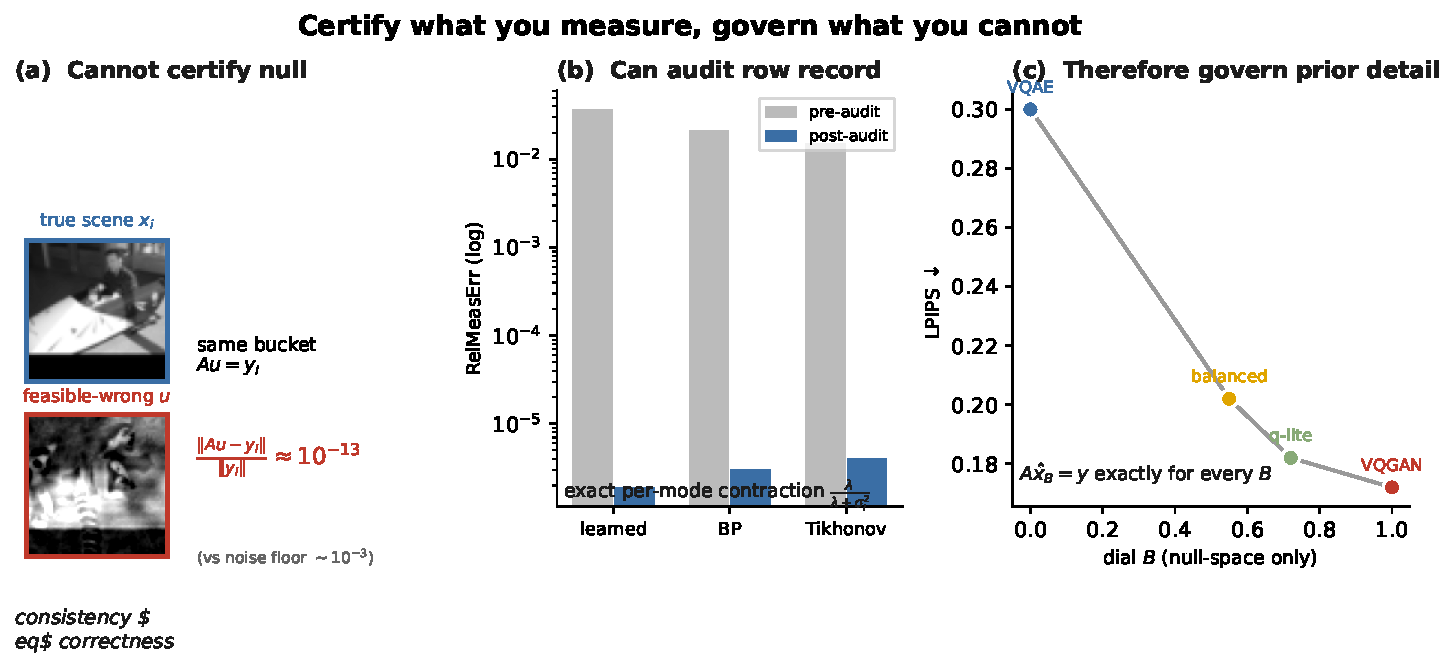
\includegraphics[width=1.0\linewidth]{METHOD_FIG1.pdf}
\caption{\textbf{The two-ledger argument.} Left (\textit{cannot}): a feasible-but-wrong image matches the target bucket record to numerical precision, so consistency cannot certify null content. Middle (\textit{can}): the audit contracts only measured modes, with factor $\lambda/(\lambda+\sigma_i^2)$. Right (\textit{therefore}): the dial injects prior detail only through $P_0$, preserving $A\hat{x}_B = y$ while moving along the perception--distortion curve (locked: LPIPS $-32.6\%$ at $-0.45$ dB, 8/8 gate).}
\end{figure}

\textbf{Contributions.}

\begin{enumerate}
\item \textbf{Constructive impossibility, cross-operator.} For any target record and donor scene we construct a feasible-but-wrong witness that preserves the record while importing the donor's null-space content. The construction transfers verbatim across operators: on $64\times64$ ghost imaging, on the real masked-Fourier fastMRI operator ($A = MF$, single-coil emulated), and on the real released SD-CASSI coded aperture, a box-legal impostor matches the record to $\sim\!10^{-16}$ --- more tightly than the clean truth matches its own noisy record (§2, §6).
\item \textbf{Exact ground-truth-free record-consistency audit.} A post-hoc audit whose residual in each measured singular mode contracts by exactly $\lambda/(\lambda+\sigma_i^2)$, image- and reconstructor-independent, certifying agreement with the recorded bucket without ground truth. On the real, data-inconsistent fastMRI U-Net the median record drift contracts from $5.86\times10^{-2}$ to $5.85\times10^{-5}$ at $\lambda = 10^{-3}$ (§3, §6).
\item \textbf{Governed null-space supply.} A scalar dial that injects prior detail strictly inside $\ker A$, preserving $A\hat{x}_B = y$ for every setting and improving locked LPIPS by 32.6\% at a bounded distortion cost. The same rule turns any published reconstructor into a governed, exactly record-consistent variant --- a data-consistent fastMRI U-Net keeps 29.42 of 29.68 dB at $R{=}4$ while restoring record consistency to $3.5\times10^{-16}$ (§4, §6).
\item \textbf{Real-operator validation and the non-uniform spectrum.} Projector identities hold in float64 on real data --- $\sim\!10^{-17}$ on real fastMRI $k$-space, $\sim\!10^{-13}$ on the real CASSI aperture, where $AA^\top = \mathrm{diag}(\Phi_s)$ makes $A^\dagger$, $P_R$, $P_0$ and the whole singular spectrum closed-form and $O(N)$. The measured CASSI spectrum spans a $528\times$ range, so the per-mode contraction spans $2\times10^4\times$ --- the empirical face of the modal-contraction theorem, invisible to flat-spectrum MRI (§6).
\item \textbf{Cross-operator third-party attribution ledger.} On the shared operators of published pipelines --- three DL-GI systems (§5), the official fastMRI single-coil U-Net, and thirteen CASSI models from the MST zoo (§6) --- we decompose each reported gain through the operator's own projectors. Twelve of the thirteen CASSI models supply 100--101\% of their gain over the $19.04$ dB min-norm ceiling from the null space with a slightly \textit{negative} row-effect (gap-net is the sole exception, 93\%); and published models are measurably record-inconsistent (0.9--12\% across the CASSI zoo; 5.9\% / 3.3\% U-Net drift), which a data-consistent estimator would not be.
\item \textbf{Limits.} A no-adaptation lemma bounds ground-truth-free dial selection (§4.5); on 429 real fastMRI+ pathology boxes the certifiable claim is \textit{coarse-certified, fine-detail-uncertified} --- the calibration region fixes a lesion's coarse presence but not its 88--94\%-null-supplied fine detail (§6).
\end{enumerate}

\medskip\noindent\fbox{\parbox{0.96\linewidth}{\textbf{Scope of all certificates.} In this paper, "certified" always means certified agreement with the recorded bucket $y$. It never means certified agreement with the unknown scene. All content in $P_0$ is prior-supplied unless additional measurements are acquired. Claims are tiered: \textit{locked} results follow a pre-specified one-shot protocol; \textit{development-level} results reuse the frozen system without a pre-specified gate. This box governs every section below.}}\medskip

\textbf{Claim hierarchy.}

\begin{center}\begin{tabular}{lcc}
\toprule
Claim & Status & Evidence \\
\midrule
Null content not certifiable from one record & theorem + witness & Prop. 1; §2 \\
Witness matches record tighter than clean truth, cross-operator & construction & GI/MRI/CASSI $\sim\!10^{-16}$; §2, §6 \\
Record consistency certifiable per mode & theorem & contraction $\lambda/(\lambda+\sigma_i^2)$; §3 \\
GT-free audit contracts real U-Net drift & external audit & $5.86\mathrm{e}{-2}\!\to\!5.85\mathrm{e}{-5}$; §6 \\
Prior supply preserves record consistency & theorem & Thm. 2; §4 \\
Governed dial: perception up at bounded cost & locked experiment & LPIPS $-32.6\%$, 8/8; §4.3 \\
Governed U-Net keeps gain at exact consistency & external audit & $29.42/29.68$ dB, drift $3.5\mathrm{e}{-16}$; §6 \\
GT-free per-image adaptation adds little & development-level & $\le 0.002$; §4.5 \\
Projector identities exact on real operators & real-operator & fastMRI $\sim\!10^{-17}$, CASSI $\sim\!10^{-13}$; §6 \\
CASSI spectrum non-uniform ($528\times$) & real-operator & $\sigma_j \in [0.009, 4.907]$; §6 \\
Published gains 93--101\% null-supplied & external audit & 3 GI + U-Net + 13 CASSI; §5, §6 \\
Published models record-inconsistent (contingent) & external audit & 0.9--12\%; 5.9\%/3.3\%; §6 \\
Coarse lesion certified, fine detail not & external audit & 429 fastMRI+ boxes; §6 \\
\bottomrule
\end{tabular}\end{center}

The locked dial experiments use signed, gray-valued computational GI operators (row-orthonormalized for the dial's operator) on $64\times64$ grayscale STL10; the real-operator legs (§6) use the exact masked-Fourier operator of NYU fastMRI single-coil $k$-space and the real released CASSI coded aperture. We do not model DMD quantization, photon budgets, or Poisson statistics; the emulated-single-coil MRI and declared-integer-shift CASSI operators keep $A$ exact rather than physically captured, and all quantitative claims are simulation- and declared-operator-level (§8).

\medskip\hrule\medskip

\section*{2. Geometry and Constructive Impossibility}

\textbf{Setup.} The forward model is $y = Ax + \varepsilon$ with $x \in \mathbb{R}^n$, $y \in \mathbb{R}^m$, $m \ll n$; in the witness and audit experiments $\varepsilon$ is i.i.d. Gaussian bucket noise with $\sigma_\varepsilon = 0.01$. The relative measurement error of a candidate $v$ against a record $y$ is $\mathrm{RelMeasErr}(v;y) = \lVert Av - y\rVert_2/\lVert y\rVert_2$.

\textbf{Theorem 1 (measurement geometry).} \textit{Let $A = U_r \Sigma_r V_r^\top$ be the compact SVD and $P_R = A^\dagger A = V_r V_r^\top$, $P_0 = I - P_R$. Then $P_R, P_0$ are orthogonal projectors splitting $\mathbb{R}^n = \mathcal{R}(A^\top) \oplus \mathcal{N}(A)$, and}

$$A P_0 = 0, \qquad A P_R = A.$$

\textit{Consequently $Ax = A P_R x$: the record is a function of the measured component alone, and the noiseless feasible set is the affine flat $\{x: Ax = y\} = A^\dagger y + \mathcal{N}(A)$.} (Proof and the rows-orthonormal special case: Appendix A.)

In the locked setting --- $n = 4096$, $m = 205$ --- the measurement-visible subspace has dimension 205 and the orthogonal null subspace has dimension 3891; these are modal degrees of freedom of the operator, not pixel subsets. Most of what the eye reads as detail is carried by the null ledger.

\subsection*{2.1 The witness construction}

\textbf{Proposition 1 (feasible-but-wrong splice).} \textit{Assume $A$ has full row rank. For any record $y \in \mathbb{R}^m$ and any donor image $x_j$, define}

$$u_j(y) = x_j - A^\dagger\big(A x_j - y\big).$$

\textit{Then}

$$A\,u_j(y) = y, \qquad P_0\,u_j(y) = P_0\, x_j, \qquad P_R\, u_j(y) = A^\dagger y.$$

\textit{The donor's null content is imported wholesale while the target record is preserved exactly.} (Proof: $AA^\dagger = I_m$ and $P_0 A^\dagger = 0$.)

One clarification governs the experiments below. The clean target $x_i$ is not expected to lie on the noisy record fiber $\{v : Av = y_i\}$ --- that is why its own residual is $O(\sigma_\varepsilon)$. The witness, by contrast, is constructed directly on that fiber, so its residual sits at floating-point scale. Figure 2 draws the construction.

The witness is also a \textit{legal image}, not only a linear-space vector. The raw splice leaves the pixel box mildly (range $[-0.34, 1.42]$, median $3\%$ of pixels outside $[0,1]$ on the dial's operator), and naive clipping does break its residual (to ${\sim}10^{-2}$). Alternating the exact fiber projection with box clipping (200 iterations; the reported object is the final clipped iterate) empirically produces a \textbf{box-constrained witness}. For 9 of 16 pairs the alternation reaches the fiber--box intersection at $\le 10^{-11}$ (8 pairs at machine precision); for the remaining 7 it stalls between $5\times10^{-6}$ and $1.5\times10^{-3}$ --- consistent with a near-empty intersection for those pairs, yet still at or below the truth's own bucket-noise residual. Every one of the 16 is a $[0,1]$-valued image whose null component is the donor's by construction and whose PSNR to the target is $19.8$ dB at the median. Any residual test loose enough to accept the noisy truth accepts a box-legal impostor; the impossibility is not an artifact of unconstrained linear algebra.

\begin{figure}[H]\centering
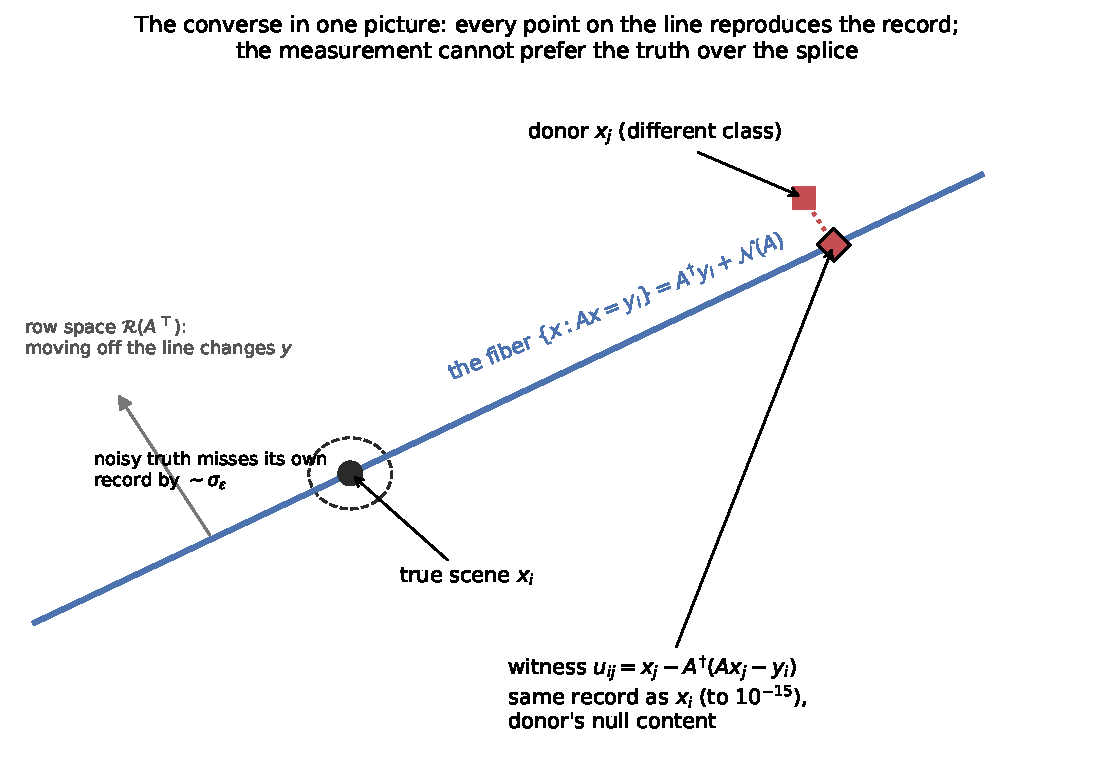
\includegraphics[width=0.8\linewidth]{WITNESS_GEOMETRY.pdf}
\caption{\textbf{The converse in one picture.} Every point on the line (the fiber $\{x: Ax = y_i\}$) reproduces the record; moving off the line is the only thing the measurement can see. The witness is the donor projected onto the fiber: it matches the record to $10^{-15}$ --- more tightly than the clean truth (dashed circle, radius $\sim\sigma_\varepsilon$) matches that same noisy record --- while carrying the donor's null content.}
\end{figure}

\subsection*{2.2 A wrong image matches the noisy record more tightly than the clean truth does}

In our 5\% instance the constructed witnesses match the noisy target record at $10^{-15}$ to $10^{-13}$ relative error, while the clean truth matches that same record only at $10^{-3}$ --- its own bucket noise. The witnesses remain visually and metrically wrong. Therefore any residual threshold loose enough to accept the truth must accept the witness.

The numbers behind this statement: on the Rademacher operator, all $16/16$ constructed cross-class pairs sit at the ${\sim}2\times10^{-15}$ scale --- the 8 reference pairs spanning $[2.16, 4.00]\times10^{-15}$ --- against truth residuals of $[3.45, 7.46]\times10^{-3}$, with witness-to-target PSNR of only $7.7$--$11.4$ dB; a featured car-versus-horse pair reads $2.93\times10^{-15}$ against the truth's $5.36\times10^{-3}$. On the same mixed-basis operator that carries the dial of §4, 40 witnesses reproduce their records at a median of $9.9\times10^{-14}$ while remaining semantically wrong (median PSNR $19.5$ dB). The two numbers measure different things: the witness's $10^{-15}$ is geometry (it is constructed on the record), while the truth's $10^{-3}$ is its own bucket noise. Operator-level details are in Appendix B.

\subsection*{2.3 A provenance warning}

The observable magnitude $|P_0\hat{x}|$ is a provenance map, not an error map. The true null error is $P_0\hat{x} - P_0 x$, and $P_0 x$ is absent from the record. Empirically the pixelwise correlation between $|P_0\hat{x}|$ and true null error is near zero; details are in Appendix F.

\medskip\hrule\medskip

\section*{3. The Record-Consistency Audit}

The null ledger cannot be certified; the measured record can be audited exactly. This section gives the audit and what it buys.

\subsection*{3.1 The audit operator}

For any reconstruction $\hat{x}$, define

$$\Pi_y^\lambda(v) = v - G_\lambda\,(Av - y), \qquad G_\lambda = A^\top(AA^\top + \lambda I)^{-1}, \quad \lambda > 0.$$

The audit needs only $(A, y, \lambda)$ --- no ground truth, no access to the reconstructor. Its correction lies in $\mathcal{R}(A^\top)$, so $P_0\,\Pi_y^\lambda(v) = P_0 v$: whatever a prior placed in the null space passes through untouched. The audit operates strictly inside the subspace the measurement is accountable for.

\subsection*{3.2 Exact modal contraction}

Applying $A$ and diagonalizing $AA^\top$, each measured mode's residual is scaled independently:

$$c_i(\lambda) = \frac{\lambda}{\lambda + \sigma_i^2}.$$

The contraction is exact, image-independent, and reconstructor-independent. In float64 the measured contraction matches the formula to $1.04\times10^{-10}$ (Rademacher operator) and $2.29\times10^{-12}$ (scrambled Hadamard); as $\lambda \to 0$ the audit becomes a hard projection onto $\{Av = y\}$.

The audit is a record-consistency certificate. It certifies agreement with the recorded bucket $y$, not with the unknown noiseless $Ax$. In a physical deployment, $\lambda$ should be chosen by a discrepancy principle or a noise model rather than driven to zero.

The factor itself is classical --- the complement of the Tikhonov filter factor (Engl, Hanke \& Neubauer 1996; Hansen 1998), and MacKay's (1992) effective-parameter summand. The contribution is its use: a post-hoc, per-record audit after arbitrary reconstructors, paired with the converse of §2 (positioning: §7, Appendix D). Its non-uniform empirical face --- a $528\times$ singular spectrum spreading the per-mode factor over four orders of magnitude --- is measured on the CASSI operator in §6.

\begin{figure}[H]\centering
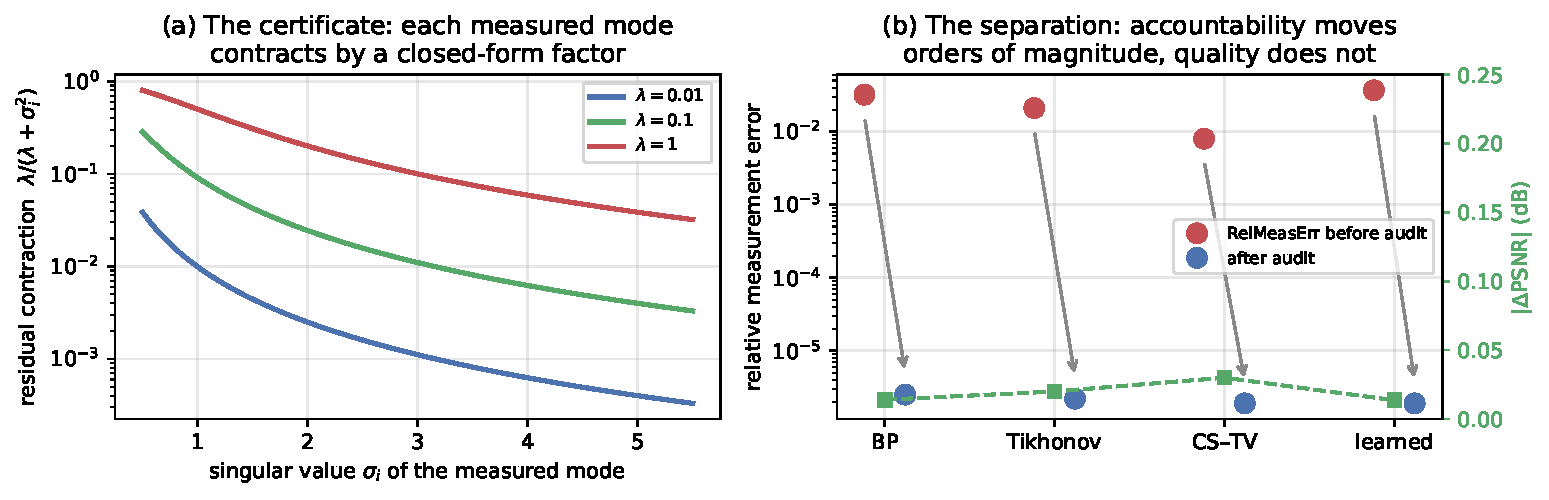
\includegraphics[width=1.0\linewidth]{CERT_SEPARATION.pdf}
\caption{\textbf{The certificate and the separation.} \textit{(a)} Each measured mode contracts by the closed-form factor $\lambda/(\lambda+\sigma_i^2)$. \textit{(b)} Applied post-hoc to four unrelated reconstructors, the audit moves measurement accountability by orders of magnitude while PSNR barely moves: the two axes decouple because $AP_0 = 0$.}
\end{figure}

\subsection*{3.3 Quality and accountability separate}

We state the separation twice, once per noise regime, because the two statements certify different objects.

\textit{Noiseless separation.} With $y = Ax$ and $e = \hat{x} - x$, we have $A\hat{x} - y = Ae = A P_R e$: the audit residual depends on the clean row-space error alone, and $\|e\|^2 = \|P_R e\|^2 + \|P_0 e\|^2$. Define the row-error share $s = \|P_R e\|^2/\|e\|^2$.

\textit{Recorded-noisy separation.} With $y = Ax + \varepsilon$, the audit residual is $A(\hat{x} - x) - \varepsilon$: a record-level quantity, not the clean row error. Equivalently, defining the record-consistent surrogate $x_y = A^\dagger y + P_0 x$, the audit certifies the row component of $\hat{x} - x_y$. In the noisy experiments the certificate is therefore a statement about the recorded fiber, while the clean-error decomposition below is used for oracle analysis only.

\textbf{Lemma 1 (row-space correction PSNR ceiling).} \textit{A correction $T$ with $T(v) - v \in \mathcal{R}(A^\top)$ can remove only $P_R e$, so it raises PSNR by at most $-10\log_{10}(1-s)$ (proof: Appendix B). Corrections that edit the null space are outside the hypothesis --- which is the content: only null-space injection can exceed the row budget, and the measurement certifies none of it.}

Trained networks sit near $s \approx 0$: re-imposing consistency is nearly free in PSNR and decisive in accountability. The audited learned reconstructor moves from $\mathrm{RelMeasErr} = 3.68\times10^{-2}$ to $1.90\times10^{-6}$ while PSNR changes by $0.014$ dB; across all 18 audited rows the residual falls three to four orders at $|\Delta\mathrm{PSNR}| \le 0.039$ dB. The image-level counterpart of $s$ is the row-energy share $\rho = \|P_R x\|^2/\|x\|^2$, which tracks the sampling rate almost exactly ($\rho \approx 0.05$ at 5\%, $0.10$ at 10\%): the operator decides how much of a scene is measurable, and the prior owns the rest.

\subsection*{3.4 What the audit catches that quality metrics cannot}

The decisive probe is operator drift. Auditing with a miscalibrated operator and evaluating against the true one, PSNR moves by $0.03$ dB while the true-operator residual rises from $1.90\times10^{-6}$ to $4.88\times10^{-2}$ --- four orders of magnitude. A quality-only pipeline reports success; the audit reports the mismatch. (Wrong-record and coordinate-shuffle probes confirm the trained reconstructor genuinely conditions on $y$; details in Appendix B.)

\medskip\hrule\medskip

\section*{4. The Governed Null-Space Dial}

The dial is not a fusion architecture. It is a provenance constraint: whatever prior is used, its contribution is projected into $\ker A$, so perceptual detail is supplied without borrowing measurement authority. We call the control \textit{governed} because it changes only what the measurement cannot certify and reports that change as prior-supplied detail.

\subsection*{4.1 Construction}

We instantiate the rule with two matched vector-quantized priors per seed: a reconstruction-trained autoencoder (VQAE, faithful but flat, contribution $d_A$) and an architecturally identical adversarially-trained prior (VQGAN, sharp detail, contribution $d_G$), both taken relative to a measurement-audited LMMSE anchor $x_0$ with $Ax_0 = y$:

$$d_A = P_0(x_A - x_0), \qquad d_G = P_0(x_G - x_0), \qquad \hat{x}_B = x_0 + P_0\big(d_A + B\,(d_G - d_A)\big).$$

\textbf{Theorem 2 (exact consistency for every $B$).} $A\hat{x}_B = A x_0 + A P_0(\cdot) = y$ \textit{for all} $B \in \mathbb{R}$. The identity that makes null content unverifiable (§2) is the identity that makes injecting it measurement-safe. Numerically the locked splits hold $\mathrm{RelMeasErr}$ at $3.6\times10^{-7}$ (float32 pipeline scale) for every operating point.

\textit{Pixel-range protocol.} The identity holds for the unclipped reconstruction. About $3\%$ of output pixels fall outside $[0,1]$; all reported residuals are computed before clipping, quality metrics (LPIPS/PSNR/SSIM) are computed on the clipped image, and figure panels are clipped only for rendering --- the clipped display object satisfies the record to ${\sim}4\times10^{-3}$, and clipping is not part of the reconstruction pipeline.

\begin{figure}[H]\centering
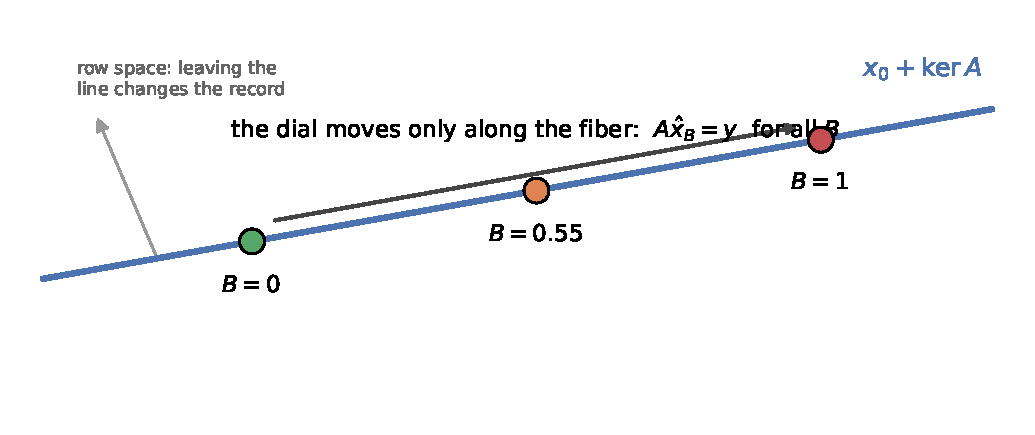
\includegraphics[width=0.8\linewidth]{DIAL_MECHANISM.pdf}
\caption{The dial moves only inside the measurement fiber. Since $AP_0 = 0$, changing $B$ changes prior-supplied null content without changing the recorded bucket.}
\end{figure}

\subsection*{4.2 The perception--distortion ladder}

Sweeping $B$ traces a monotone ladder on the perception--distortion plane (Blau \& Michaeli 2018):

\textbf{Table 1. Locked-split means (512 images, 3 seeds).} All VQAE/VQGAN endpoints are row-space anchored, $x_0 + P_0(x_\cdot - x_0)$, not raw network outputs.

\begin{center}\begin{tabular}{lccccc}
\toprule
Operating point & LPIPS $\downarrow$ & PSNR (dB) $\uparrow$ & RMSE $\downarrow$ & SSIM $\uparrow$ & RAPSD $\downarrow$ \\
\midrule
LMMSE anchor $x_0$ & 0.404 & 22.80 & 0.076 & 0.629 & 0.0041 \\
Projected VQAE endpoint ($B=0$) & 0.300 & 23.13 & 0.073 & 0.657 & 0.0030 \\
\textbf{Balanced} ($B\!\approx\!0.55$) & \textbf{0.202} & 22.69 & 0.077 & 0.633 & 0.0027 \\
Quality-lite ($B\!\approx\!0.72$) & 0.182 & 22.21 & 0.081 & 0.609 & 0.0024 \\
Projected VQGAN endpoint ($B=1$) & 0.172 & 21.43 & 0.089 & 0.571 & 0.0019 \\
\bottomrule
\end{tabular}\end{center}

From the projected VQAE endpoint onward every column is monotone: each increment of $B$ trades pixel fidelity for perceptual and spectral realism at fixed measurement fidelity. The balanced point captures roughly three-quarters of the available LPIPS range while holding PSNR within half a decibel of VQAE. A dense 21-point sweep is smooth, with strictly monotone LPIPS and no interior perceptual optimum (Appendix C).

\begin{figure}[H]\centering
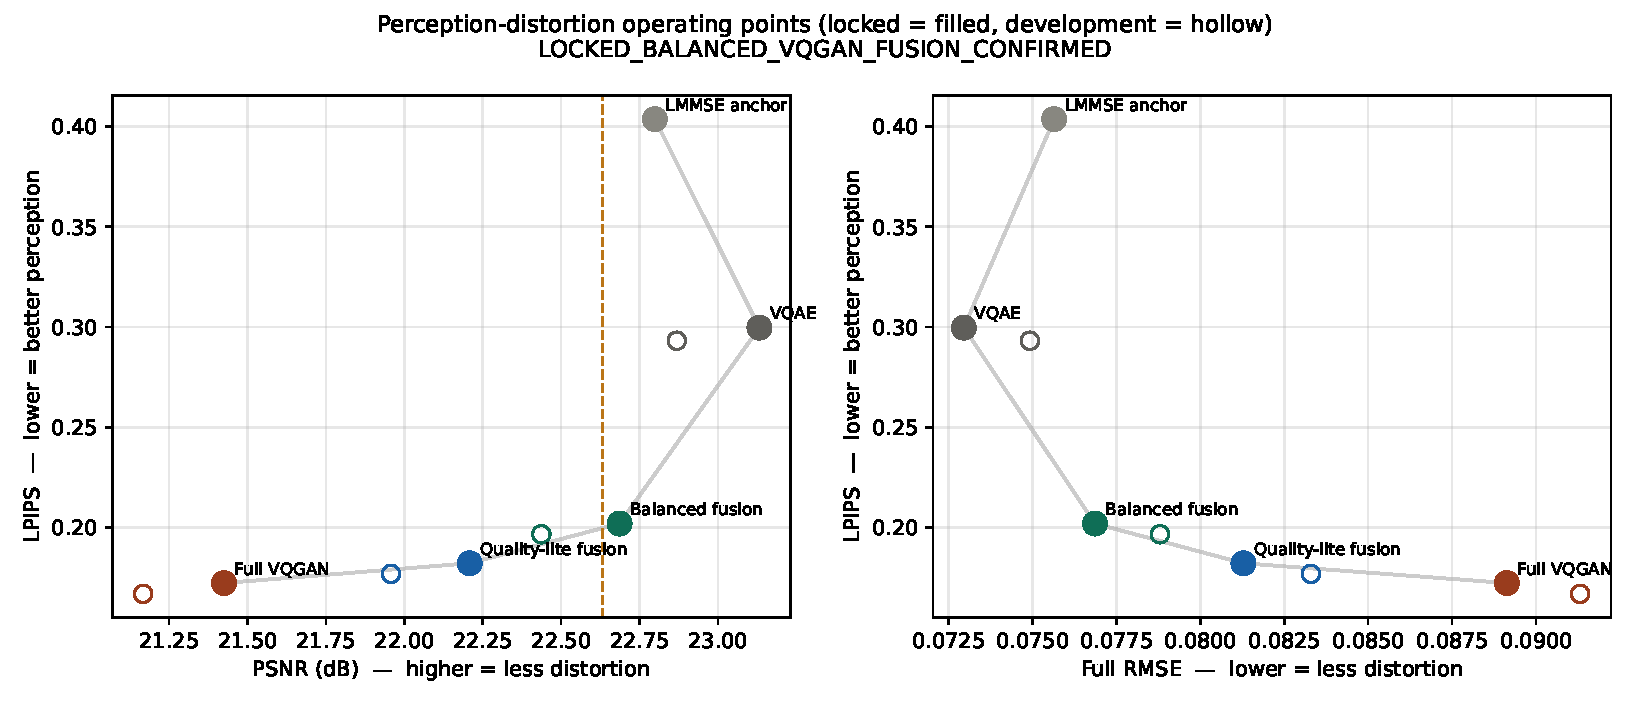
\includegraphics[width=0.9\linewidth]{PARETO_FIGURE.pdf}
\caption{\textbf{The ladder on the perception--distortion plane.} Named operating points of Table 1; every point satisfies $A\hat{x} = y$, so the trade moves entirely within the null ledger.}
\end{figure}

\subsection*{4.3 Locked confirmation}

\medskip\noindent\fbox{\parbox{0.96\linewidth}{\textbf{Locked protocol.} Dataset: STL10 grayscale $64\times64$; operator: 5\% ($m=205$) --- 1 DC row, 128 low-frequency DCT rows, 56 low-sequency Hadamard rows, 20 random rows, orthonormalized, seed 772001. Splits by raw-SHA256 deduplication: train 20,000 / validation 512 (selects $B$) / development 512 / locked 512, raw-hash disjoint from all previously consumed hashes. $B$ frozen per seed $\{0.55, 0.55, 0.50\}$ before the locked read. Gate (8 pre-specified conditions): relative LPIPS gain $\ge 5\%$; LPIPS CI $<0$; seed agreement; PSNR within $0.5$ dB; RMSE within $0.005$; RAPSD not worse; $\mathrm{RelMeasErr} \le 10^{-5}$; hash-disjointness audit. Evaluation: one shot. Full details: Appendix C.}}\medskip

The gate passes 8/8. Balanced fusion improves LPIPS by $-0.0977$ (CI $[-0.1016, -0.0940]$; $32.6\%$) at $-0.45$ dB PSNR and $+0.0039$ RMSE, with spectral realism improving and all three seeds agreeing; $A\hat{x}_B = y$ holds at numerical precision throughout. The development split, scored before the locked run, gives $-0.0965$ ($32.9\%$) --- the effect is stable, not selected. Post-hoc, distribution-level KID falls from $0.119$ to $0.043$.

\begin{figure}[H]\centering
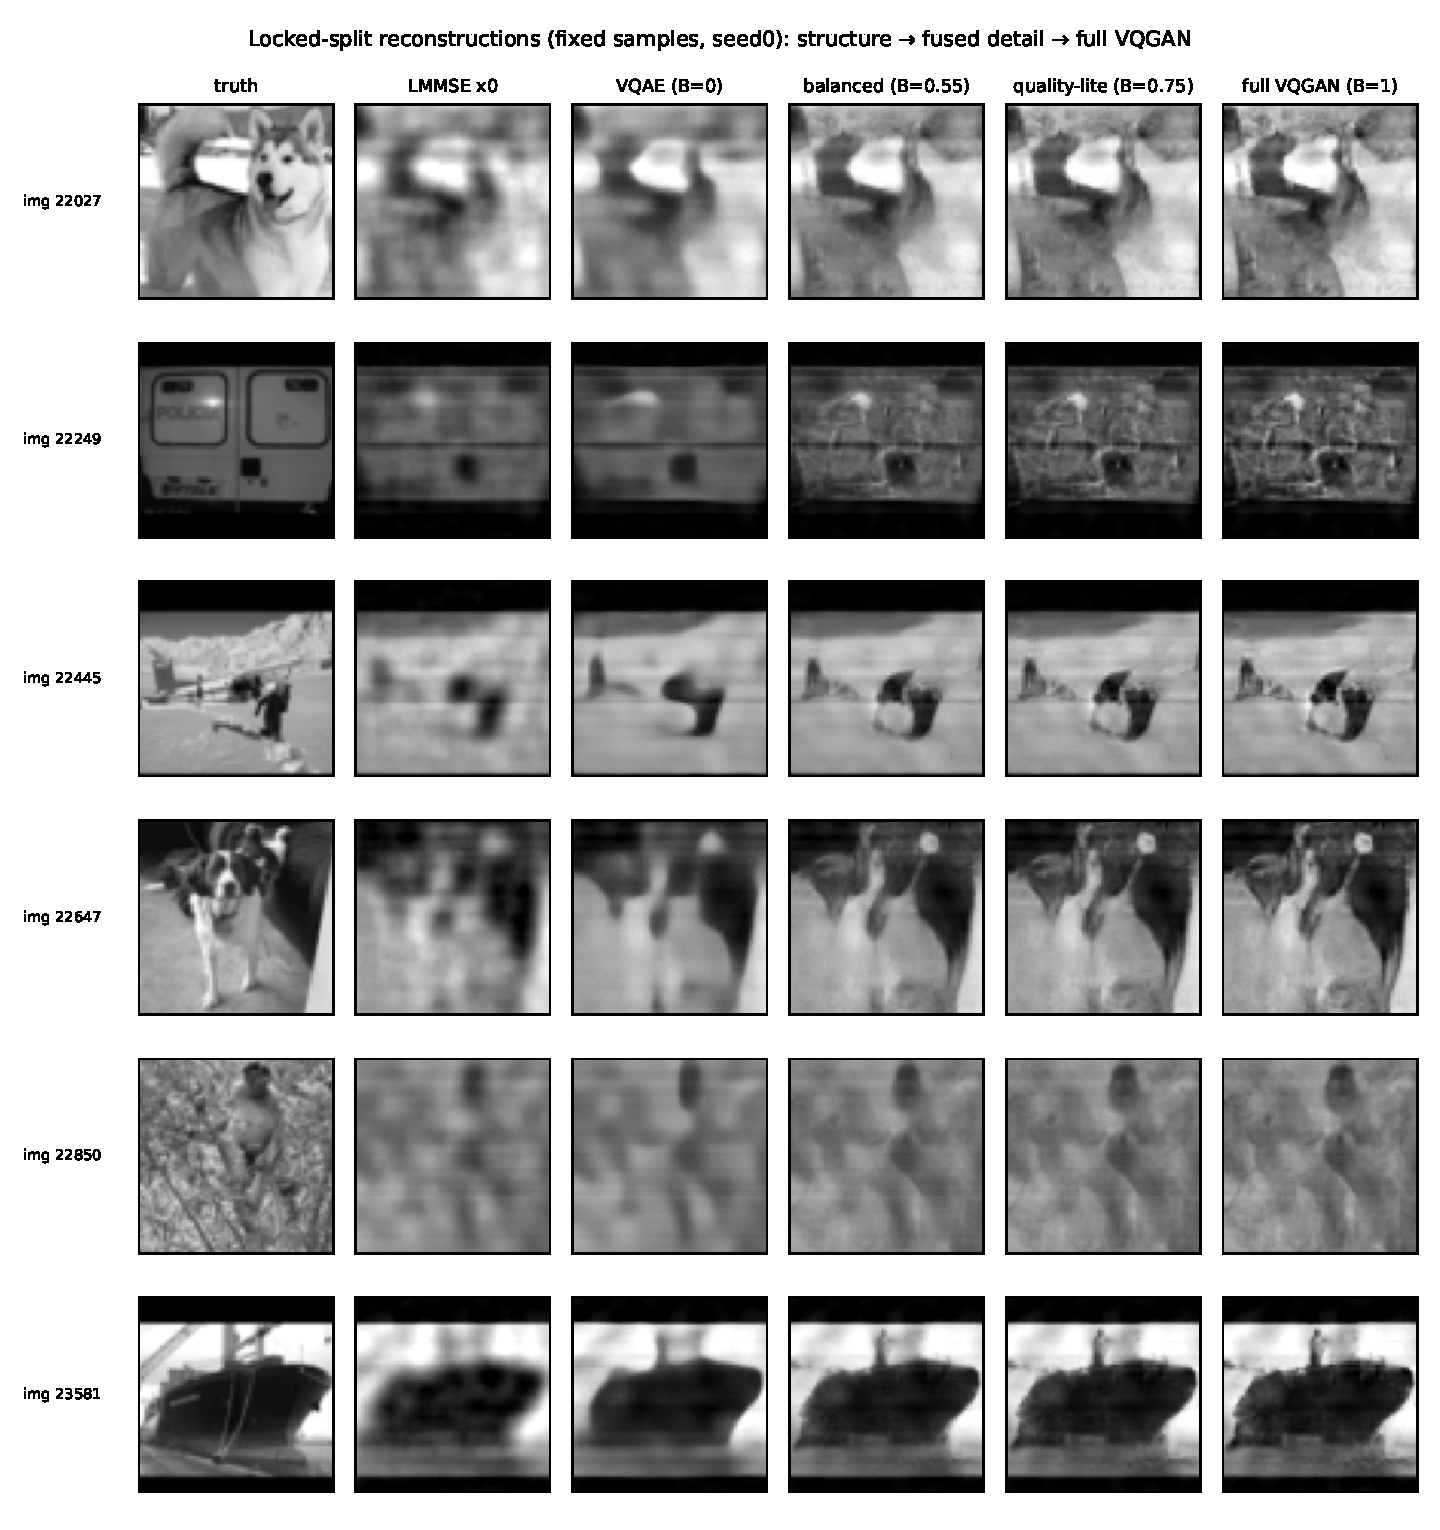
\includegraphics[width=1.0\linewidth]{QUALITATIVE_GRID.pdf}
\caption{\textbf{Locked-split reconstructions across the ladder.} Moving right adds perceptual detail; every column reproduces the identical bucket record. The added detail lives in the null ledger.}
\end{figure}

\subsection*{4.4 Robustness of the operating point}

The advantage travels. At 2\%, 5\%, and 10\% sampling the balanced dial improves LPIPS by $29$--$34\%$ relative to VQAE with all seeds agreeing (development-level; Table 2). Under bucket noise the balanced point degrades gracefully and overtakes full VQGAN at $\sigma_\varepsilon = 0.02$ --- the recommended setting is also the robust one (Table 3). The gain is broad: LPIPS improves on $99.0\%$, $97.5\%$, and $99.2\%$ of locked images across seeds, and the rare regressions concentrate on man-made periodic structure where a natural-image prior is a known mismatch.

\textbf{Table 2. Cross-rate generalization (development-level, 3 seeds/rate).}

\begin{center}\begin{tabular}{lccc}
\toprule
Rate & $\Delta$LPIPS vs VQAE & Relative & $\Delta$PSNR (dB) \\
\midrule
2\% ($m=82$) & $-0.116$ & $29.3\%$ & $-0.39$ \\
5\% ($m=205$, locked) & $-0.098$ & $32.6\%$ & $-0.45$ \\
10\% ($m=410$) & $-0.076$ & $34.2\%$ & $-0.43$ \\
\bottomrule
\end{tabular}\end{center}

\textbf{Table 3. LPIPS under bucket noise (development-level, $B$ frozen).}

\begin{center}\begin{tabular}{lccc}
\toprule
$\sigma_\varepsilon$ & VQAE & Balanced & Full VQGAN \\
\midrule
0.00 & 0.300 & 0.202 & 0.172 \\
0.01 & 0.297 & 0.195 & 0.176 \\
0.02 & 0.295 & \textbf{0.197} & 0.204 \\
0.05 & 0.304 & \textbf{0.250} & 0.293 \\
\bottomrule
\end{tabular}\end{center}

\subsection*{4.5 Why the dial is one scalar: the no-adaptation lemma}

\textbf{Lemma 2 (no-adaptation).} \textit{(i) With a noiseless record, any selection rule $g(A, y)$ is constant on each fiber $\{x: Ax = y\}$: no such rule can distinguish fiber-mates. (ii) In the general model, for $B^\star \in L^2$ and squared loss on the weight, the best record-measurable selector is the conditional mean}

$$g^\star(y) = \mathbb{E}\big[B^\star(X) \mid Y = y\big], \qquad \inf_g \mathbb{E}\big[(g(Y) - B^\star(X))^2\big] = \mathbb{E}\big[\operatorname{Var}(B^\star(X) \mid Y)\big],$$

\textit{so the irreducible adaptation error is the oracle's conditional variance given the record.} (Proof: (i) fiber-mates share $y$, hence share $g$; (ii) is the conditional-expectation projection theorem. $\blacksquare$) Squared loss on the weight is an analysis device; the evaluation below scores LPIPS regret directly.

The lemma does not say $B(y)$ cannot vary across records; it says it cannot distinguish fiber-mates, so the best achievable adaptation is the fiber-conditional mean of the oracle, not the oracle. It excludes exactly one thing: one-record, ground-truth-free, fixed-operator adaptation of null content. Its value is the pairing with measurement. Empirically the $y$-predictable component is worth essentially nothing here [development-level]: a feature-based per-image selector recovers the oracle only through a global shift of $B$, with excess $\le 0.002$ LPIPS over a matched-PSNR constant and feature--oracle correlations $|\rho| \le 0.24$. Richer parameterizations (16-band frequency weights, a learned gate) also lose to the scalar under the registered rule. Frameworks that do recover null information import structure beyond one record --- group equivariance or operator diversity (Chen et al. 2021; Tachella et al. 2023). Held-out measurements can likewise break the fiber and estimate null error directly; that is classical compressed-sensing cross-validation (Ward 2009), not a contribution of this paper.

\begin{figure}[H]\centering
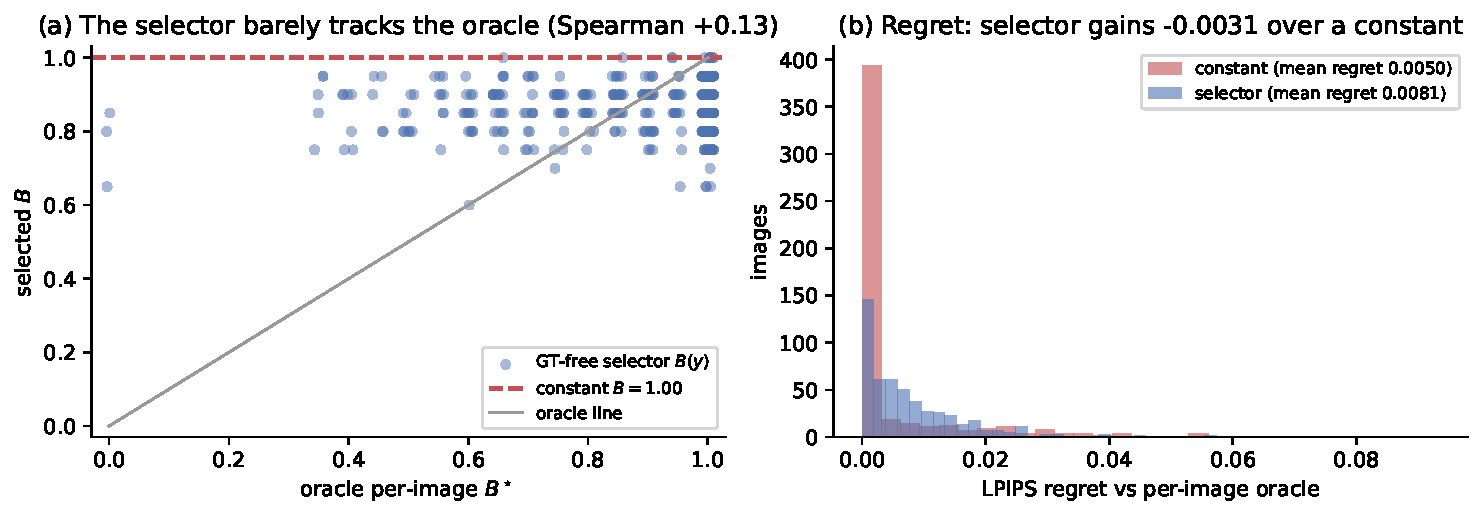
\includegraphics[width=0.95\linewidth]{NOADAPT_EMPIRICAL.pdf}
\caption{\textbf{The lemma, empirically.} \textit{(a)} The ground-truth-free selector's per-image choice $B(y)$ barely tracks the per-image oracle $B^\star$ (Spearman $+0.13$); its spread hugs a constant. \textit{(b)} LPIPS regret against the per-image oracle: the validation-optimal \textit{constant} matches or beats the selector (mean regret $0.0050$ vs $0.0081$) --- per-record adaptation from $y$ alone buys nothing here, as Lemma 2 predicts [development-level].}
\end{figure}

\medskip\hrule\medskip

\section*{5. External Check: Projector Forensics of Published Pipelines}

We treat this section as an external validity check, not as a new theorem. On each of three published DL-GI pipelines --- pretrained+fine-tuned (Wang et al. 2022a), untrained DIP on real measured speckle (GIDC; Wang et al. 2022b), and self-supervised on a genuinely noisy record (Noise2Ghost; Manni et al. 2025) --- we take \textbf{the paper's own released or measured operator and its own code}, and decompose the published improvement into row-space repair and null-space supply through the exact projectors of that operator.

The \textit{range ceiling} used below is the PSNR of the oracle row-space image $P_R x$ under the audited operator and preprocessing --- the best possible score of an estimator whose output contains no truth-aligned null component. It is an accounting reference, not a physical limit, and all attributions are relative to the min-norm reference. Across all three pipelines, row repair saturates early; headline PSNR above the range ceiling is paid from the null ledger. The split differs by method --- $61/39$, $60/40$, and $5/95$ row/null --- but the ledger structure is common, and the terminal error is $93$--$97\%$ null in every case (Figure 8). Two findings deserve their own sentences. For the original experimental GIDC scene no ground truth exists, so we decompose the reconstruction's \textit{content}, not its error: $43.8\%$ of its centered structure lies in the null space of the measured speckle operator. This \textit{upper-bounds} the super-resolved content --- the null space contains both beyond-diffraction structure and ordinary unsampled in-band structure --- so the ledger locates the super-resolution claim without measuring its exact size. To obtain an \textit{error} attribution we then substitute a known scene through the same measured patterns and code path, giving the $60/40$ split. And the noisy-record case shows real in-range denoising ($42\%$ below the noisy pseudo-inverse) that accounts for only ${\sim}5\%$ of the total gain.

\textbf{Table 4. Audit provenance (mini; full reproducibility table in Appendix E).}

\begin{center}\begin{tabular}{lccc}
\toprule
Pipeline & Operator status & GT status & Attribution \\
\midrule
PEDL & released learned patterns & known (sim) & full error split \\
GIDC & measured speckle & original: none; substituted known-GT & content split + substituted error split \\
Noise2Ghost & released sim masks & known, noisy record & full error split \\
\bottomrule
\end{tabular}\end{center}

\begin{figure}[H]\centering
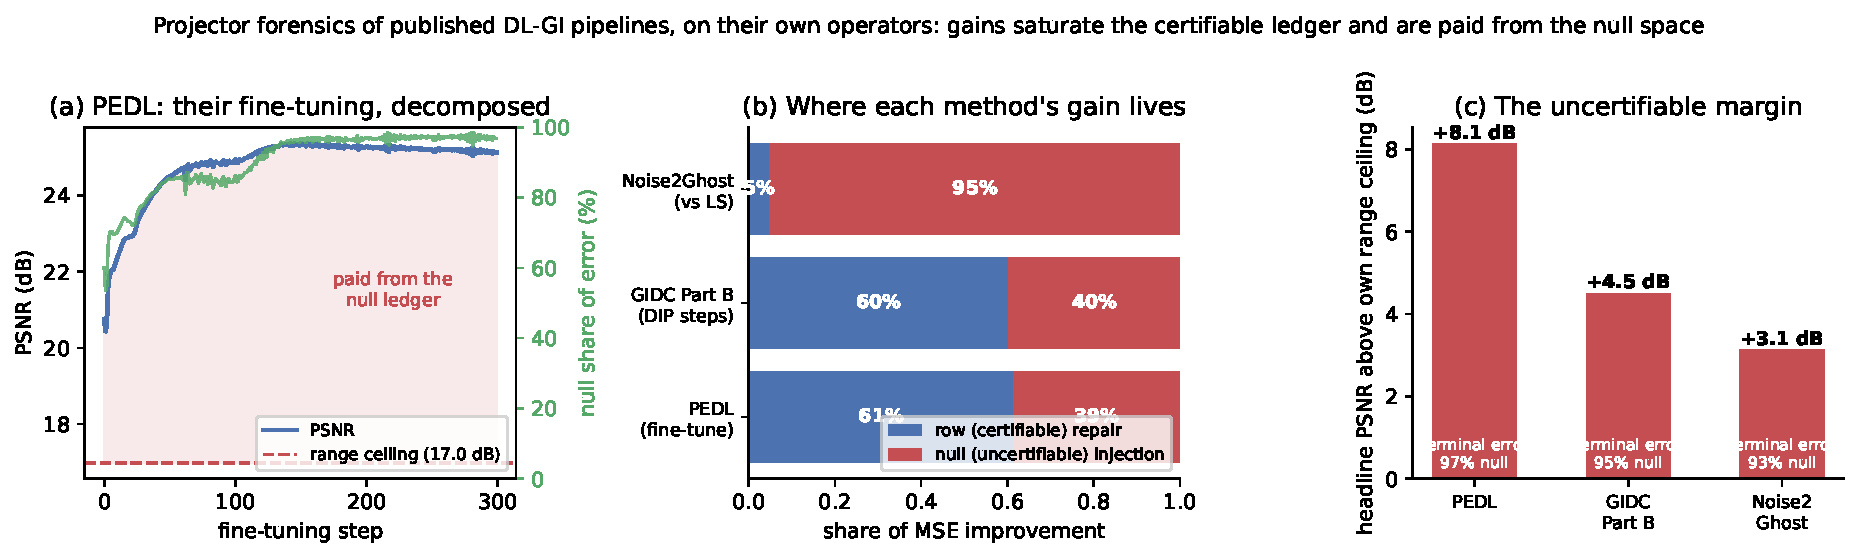
\includegraphics[width=1.0\linewidth]{FORENSICS_CROSS_TARGET.pdf}
\caption{\textbf{Three paradigms, three operators, one structure.} \textit{(a)} A fine-tuning trajectory decomposed per step: PSNR rises past the operator's range ceiling --- everything above it is paid from the null ledger. \textit{(b)} Attribution of each method's improvement: row repair vs null supply. \textit{(c)} Every headline stands $+3.1$ to $+8.1$ dB above its own range ceiling with terminal error $93$--$97\%$ null.}
\end{figure}

The audit itself survives the transfer to physical hardware [development-level]: applied on GIDC's measured speckle operator to the substituted-GT reconstruction, the record-consistency audit drives the residual from $3.0\times10^{-3}$ to $3.0\times10^{-15}$ at a PSNR change of $+0.20$ dB, and the measured per-mode contraction matches $\lambda/(\lambda+\sigma_i^2)$ to $3.5\times10^{-11}$ in float64 --- the closed form holds on a physically measured, uncalibrated-scale operator ($\sigma_i \in [511, 26607]$), not only on designed ones.

\medskip\noindent\fbox{\parbox{0.96\linewidth}{\textbf{Audit provenance and caveats.} All three audits use released code (run unmodified where the toolchain permits) and the papers' own operators: released learned patterns (verified against the shipped record to $1.2\times10^{-7}$), physically measured speckle (calibration error inherited by the attribution), and released simulation masks. The direction of the finding is partially forced by construction: most \textit{degrees of freedom} are null at these sampling rates, the min-norm reference has a $100\%$-null terminal error, and an exactly record-consistent estimator's residual error lies wholly in the null space. (These operators do capture most scene \textit{energy}: the audited scenes carry only $10$--$17\%$ of their energy in the respective null spaces.) The quantitative splits and their agreement, not the direction, are the content. Attribution is stated relative to the min-norm reference. Per-pipeline decompositions, the summary table, and a reproducibility table (code source, operator source, GT status, caveats per pipeline): Appendix E.}}\medskip

\medskip\hrule\medskip

\section*{6. Real Operators: Accelerated MRI and Snapshot Spectral Imaging}

The ghost-imaging account of §2--§5 rests on one geometric fact --- the record fixes $P_R x$ and leaves $P_0 x \in \ker A$ unconstrained --- and on one closed form, the modal contraction $c_i(\lambda)=\lambda/(\lambda+\sigma_i^2)$ of §3.2. Neither is special to single-pixel optics. We now instantiate the whole framework --- projector identities, feasible-but-wrong witness, GT-free audit, and third-party forensic ledger --- on two operators from other undersampled modalities: masked-Fourier MRI and snapshot spectral CASSI. We keep the paper's honest scope: both legs are declared-operator, emulated-single-coil, Gaussian-noise studies; the point is not a new physical experiment but that the accountability boundary transfers, verbatim, to operators built from \textit{real} released measurement systems.

The two modalities bracket §3.2. Masked-Fourier MRI has an orthonormal, flat singular spectrum ($\sigma_i \equiv 1$), so its modal contraction collapses to a \textit{single} value and §3.2 has nothing to display; CASSI has an extreme non-uniform spectrum and turns the theorem into a picture. The pair therefore does double duty: MRI shows the framework holding where the geometry is benign and clinically familiar, CASSI shows the modal-contraction spectrum in a form flat-spectrum imaging cannot exhibit.

\subsection*{6.1 Masked-Fourier MRI on real $k$-space}

We emulate single-coil accelerated MRI with the exact operator $A = MF$ --- the 2-D Fourier transform $F$ followed by a Cartesian undersampling mask $M$ --- on real NYU fastMRI knee $k$-space, with zero training. Because $A$ is a subsampled unitary, both projectors are closed-form: $P_R = A^\dagger A = F^{-1} M F$, $P_0 = I - P_R$. On real measured $k$-space the projector identities hold to ${\sim}10^{-17}$ in float64, and the emulated-single-coil ground truth $|\mathrm{crop}(\mathrm{ifft2c}(k))|$ reproduces to correlation $1.00000$.

\textbf{The witness transfers.} The §2 construction --- a feasible-but-wrong record twin --- reappears unchanged. Two \textit{different} knees are forced to share one identical $R{=}8$ (nominal; effective $6.9\times$ after the auto-calibration region) undersampled record: the two records match to median $2.9\times10^{-16}$, and a magnitude-legal, $[0,1]$-projected POCS witness matches to $2.5\times10^{-16}$. The witness is a visibly different knee at $20.3$ dB PSNR to the target, yet is measurement-indistinguishable from it. As in §2, consistency is not correctness; the geometry is the same, only the operator changed.

\textbf{Forensics on the official pipeline.} We run the §5 ledger against the released fastMRI single-coil U-Net (chans $=256$, wired from the shipped state dict). Here the accounting reference is exact, not estimated: the zero-filled reconstruction \textit{equals} $P_R x_\text{gt}$, so its magnitude PSNR \textit{is} the range ceiling. At $R{=}4$ (eff. $3.7\times$) the ceiling is $26.70$ dB and the U-Net reaches $29.68$ dB, a $+2.98$ dB gain that is $91\%$ null-supplied; at $R{=}8$ (eff. $6.9\times$) the ceiling is $24.32$ dB, the U-Net $25.42$ dB, gain $+1.09$ dB, $92\%$ null. As in the GI forensics of §5, the headline sits \textit{above} the operator's range ceiling and the surplus is paid from the null ledger --- but here the U-Net also drifts off the record it was given ($5.9\%$ at $R{=}4$, $3.3\%$ at $R{=}8$), which undersampling does not entail. A \textit{governed} data-consistent variant $A^\dagger y + P_0 x_\text{UNet}$ --- the null-space dial of §4 applied post-hoc --- keeps almost all of the gain ($29.42$ vs $29.68$ dB at $R{=}4$) at \textit{exact} record consistency (drift $3.5\times10^{-16}$). The GT-free audit of §3 then contracts the U-Net's record drift by exactly $\lambda/(\lambda+1)$ --- the flat-spectrum collapse of the §3.2 factor --- from median $5.86\times10^{-2}$ to $5.85\times10^{-5}$ at $\lambda=10^{-3}$, per-mode deviation $\le10^{-15}$.

\textbf{A governed certified decision.} On $429$ real fastMRI+ pathology bounding boxes we push the framework to a decision. The auto-calibration region certifies the \textit{coarse} lesion --- full-box null-energy median $13.5\%$ at $R{=}8$, $18.4\%$ at $R{=}16$ --- but the \textit{fine detail} inside the box is $88.4\%$ ($R{=}8$) / $93.8\%$ ($R{=}16$) null-supplied. A governed null-space edit therefore changes a soft-tissue lesion's fine-detail contrast by $-43\%$ while $Ax=y$ holds to $3.6\times10^{-16}$. We state the honest scope plainly: at clinical $4$--$8\times$ the calibration region retains the diagnostic low-frequency content, so there is no "erase the lesion" --- the certifiable claim is \textit{coarse-certified, fine-detail-uncertified}, not lesion deletion (full decomposition and the decision figure: Appendix E).

\subsection*{6.2 CASSI on the real released coded aperture}

Single-disperser CASSI shifts, masks and sums a $28$-band cube into a $256\times310$ snapshot --- a $23.1\times$ undersampling --- through the shift-mask-sum operator $A$. We build $A$ from the \textit{real released} TSA-Net gray coded aperture (fill $0.563$). This operator has a rare exact structure: $AA^\top = \operatorname{diag}(\Phi_s)$ is diagonal, so $A^\dagger$, $P_R$, $P_0$ and the entire singular spectrum are closed-form, $O(N)$, with no SVD. The projector identities hold to ${\sim}10^{-13}$ in float64.

\textbf{The non-uniform spectrum: §3.2 made visible.} The singular values $\sigma_j=\sqrt{\Phi_s}$ over $79{,}360$ measured detector modes span $[0.009,\,4.907]$ (median $3.51$) --- a $528\times$ ratio. The per-mode audit contraction $\lambda/(\lambda+\sigma_j^2)$ at $\lambda=10^{-3}$ therefore spans $[4.15\times10^{-5},\,9.21\times10^{-1}]$, a $2\times10^{4}$ spread --- precisely the modal-contraction theorem of §3.2, where masked-Fourier MRI (§6.1) collapses to the single value $9.99\times10^{-4}$. This is the empirical face of the closed form: the same audit that is one scalar under a flat spectrum resolves into a full graded profile under a non-uniform one.

\begin{figure}[H]\centering
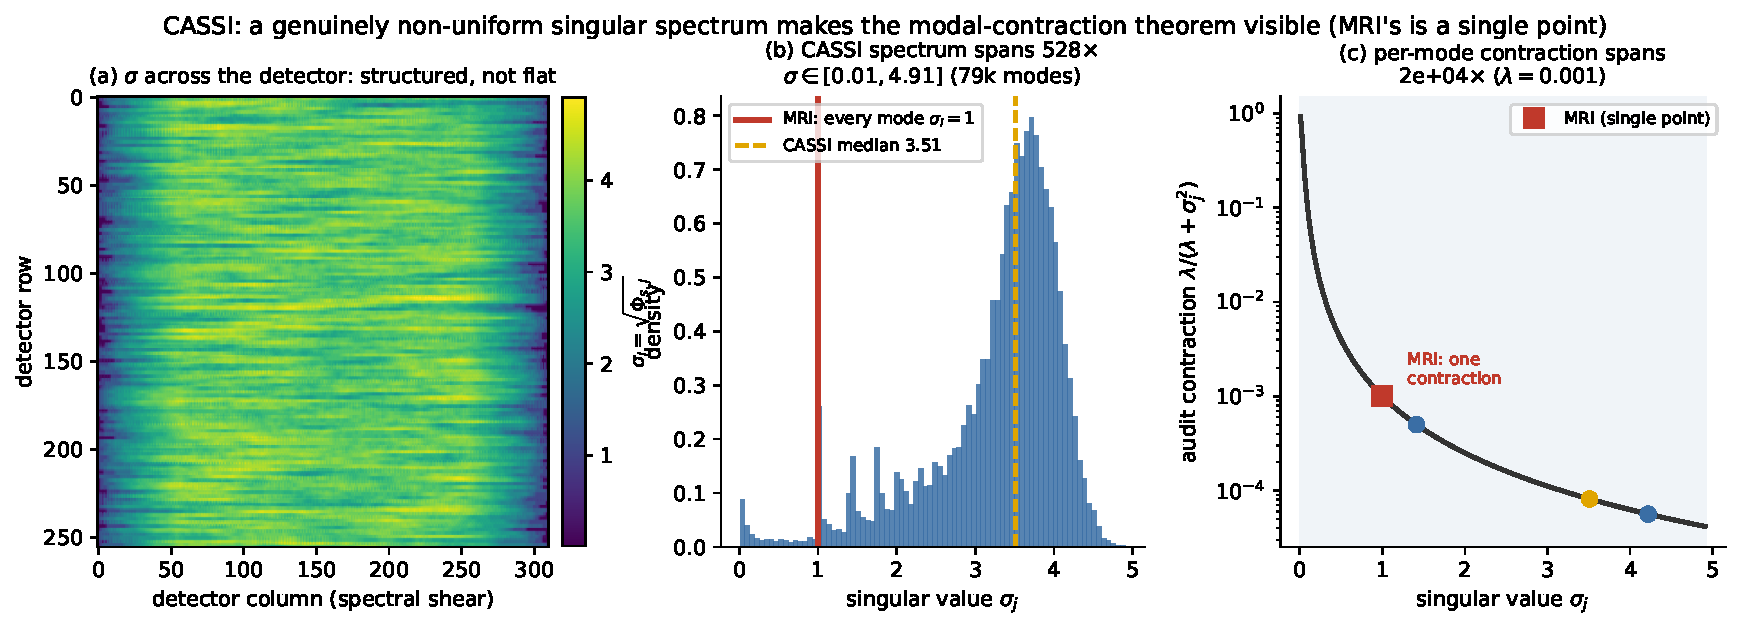
\includegraphics[width=1.0\linewidth]{CASSI_SPECTRUM.pdf}
\caption{\textbf{The modal-contraction theorem, made visible.} The CASSI singular spectrum $\sigma_j=\sqrt{\Phi_s}$ over $79{,}360$ detector modes spans a $528\times$ range; the per-mode audit factor $\lambda/(\lambda+\sigma_j^2)$ of §3.2 spreads across four orders of magnitude, where flat-spectrum masked-Fourier MRI (§6.1) collapses to a single point (dashed).}
\end{figure}

\textbf{The witness transfers.} Two \textit{different} spectral scenes are forced to share one identical $23\times$ coded snapshot: matched to median $1.7\times10^{-16}$, with a box-legal ($[0,1]$) POCS witness to $1.9\times10^{-3}$. The witness carries the donor's null-space spectral content, so the two scenes' per-pixel spectra differ visibly under an identical snapshot --- the §2 impossibility, now in the spectral channel.

\begin{figure}[H]\centering
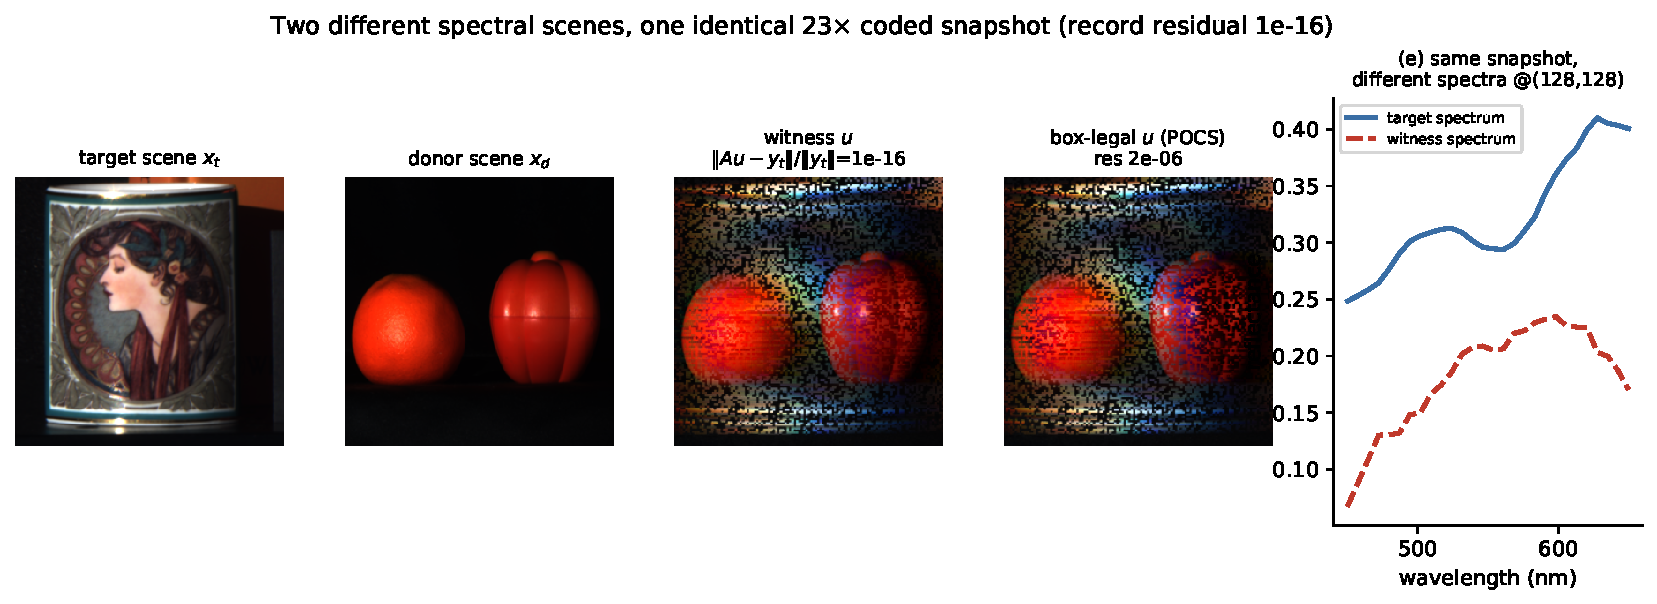
\includegraphics[width=1.0\linewidth]{CASSI_WITNESS.pdf}
\caption{\textbf{Two spectra, one snapshot.} Two spectrally distinct scenes matched to an identical $23\times$ CASSI snapshot (median $1.7\times10^{-16}$). Per-pixel spectra (insets) differ visibly, yet the coded records are indistinguishable: measurement consistency does not fix the spectral cube.}
\end{figure}

\textbf{Forensics over thirteen published models.} We run the §5 ledger across $13$ published reconstruction models from the MST model zoo on the shared operator, with the wiring validated by reproducing each model's published simulation PSNR (MST-S $34.38$ vs $34.26$; HDNet $35.06$ vs $34.97$; BIRNAT $37.73$ vs $37.58$; DAUHST-9stg $38.18$ vs $38.36$). The min-norm $A^\dagger y$ range ceiling is $19.04$ dB, and \textit{twelve of the thirteen} models supply $100$--$101\%$ of their PSNR gain over that ceiling from the null space, with the row-effect slightly \textit{negative} --- the models mildly corrupt the measured component rather than repairing it; GAP-Net is the sole exception ($93\%$ null, a positive row-effect, and the largest record drift). The entire decade of progress, TSA-Net $31.67 \to$ DAUHST-9stg $38.18$ ($+6.5$ dB), happens wholly in the null ledger, and the models are $0.9$--$12\%$ record-inconsistent. This mirrors the GI ledger of §5 in a modality with $23\times$ more undersampling and $13\times$ more pipelines.

\begin{figure}[H]\centering
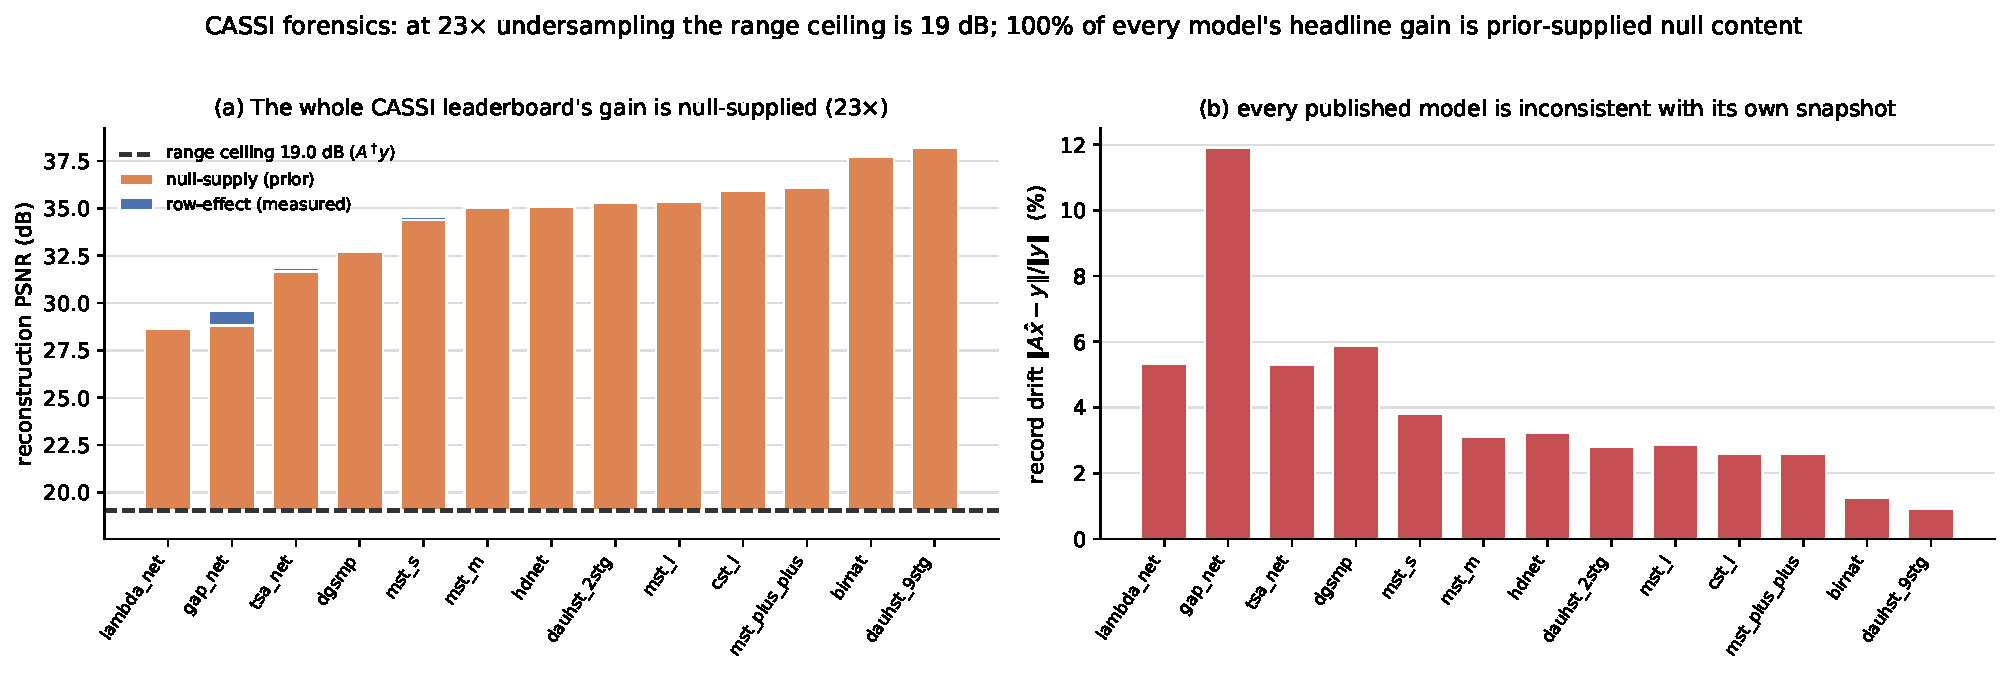
\includegraphics[width=1.0\linewidth]{CASSI_FORENSICS.pdf}
\caption{\textbf{A decade of SOTA in the null ledger.} Thirteen published CASSI models decomposed on their shared operator against the $19.04$ dB min-norm range ceiling. Twelve of the thirteen gains (TSA-Net $\to$ DAUHST-9stg, $+6.5$ dB) are $100$--$101\%$ null-supplied (GAP-Net the exception at $93\%$); the row-effect is slightly negative (models move the measured component \textit{away} from $A^\dagger y$) and each is $0.9$--$12\%$ record-inconsistent.}
\end{figure}

\subsection*{6.3 What the two operators establish together}

\textbf{The bracket.} MRI and CASSI bracket the geometry of §3.2 from both ends. MRI is flat and well-conditioned ($\sigma_i\equiv1$), clinically familiar, and its modal contraction is a single scalar; CASSI is extreme and non-uniform ($528\times$), and its contraction is a four-order-of-magnitude profile. The witness, the projector identities, the GT-free audit, and the forensic ledger hold at both ends and everywhere the operator can sit between them. Together with the GI operator of §5, the account now spans single-pixel optics, Fourier imaging, and dispersive spectral imaging on operators drawn from three real measurement systems.

\textbf{Tautology defense.} As §5's caveat box already concedes, part of the direction is forced at $m\ll n$, and we keep definitional and contingent apart. That a record-consistent estimator's error is null-dominated is \textit{not} a finding: $AP_0=0$ and the orthogonal split $\|e\|^2=\|P_R e\|^2+\|P_0 e\|^2$ make it true by construction whenever most degrees of freedom are unsampled, and the min-norm reference has a $100\%$-null terminal error by definition. What is \textit{contingent} --- not entailed by $m\ll n$, and therefore the actual content --- is fourfold: (i) the measured record-\textit{inconsistency} of the published models ($5.9$/$3.3\%$ for the U-Net, $0.9$--$12\%$ across the CASSI zoo), which a data-consistent estimator would not have; (ii) the slightly \textit{negative} row-effect, models moving the measured component \textit{away} from $A^\dagger y$; (iii) the specific $528\times$ non-uniform CASSI spectrum, an operator fact rather than a consequence of sampling rate; and (iv) the cross-model, cross-modality \textit{agreement} of the split. The ledger is accounting, not accusation: it locates where each pipeline's quality is manufactured, and the governed variants of §6.1 show the same quality can be retained at exact record consistency. Positioning against the range--null and null-space-injection prior art is §7 and Appendix D.

\medskip\hrule\medskip

\section*{7. Related Work}

\begin{center}\begin{tabular}{lcc}
\toprule
Prior line & What it owns & What this paper adds \\
\midrule
Backus--Gilbert; Barrett--Myers & Linear estimability, null functions & Per-instance witness; GI governance protocol \\
MacKay; Tikhonov filter factors & Modal factors, effective parameters & Per-record post-hoc audit role \\
Null-space networks; DDNM; NPN/GSNR; RND-SCI & Data-consistent null filling (incl. inside CASSI) & Consistency read as non-certification; metered prior content \\
Bhadra; Gottschling; Antun; Iagaru & Hallucination limits, kernel instability & Constructive record-tight witness; governed dial; field audit \\
Shang et al. (Bayesian SPI); conformal UQ & GT-free \textit{statistical} uncertainty of DL reconstructions & Exact operator-level record certificate; measured-vs-prior split \\
Perception--distortion; CodeFormer/ESRGAN knobs & Fidelity--quality controls & Knob acts strictly in $P_0$, preserving the record exactly \\
\bottomrule
\end{tabular}\end{center}

\textbf{Ghost imaging.} The modality began with entangled-photon correlation imaging (Pittman et al. 1995); thermal-light and computational variants (Gatti et al. 2004; Ferri et al. 2005; Shapiro 2008; Bromberg et al. 2009; Duarte et al. 2008; Edgar et al. 2019) established the single-pixel operator this paper audits. Learned GI reconstructors (Lyu et al. 2017; He et al. 2018; the three pipelines of §5) buy large quality gains whose provenance is exactly what the two-ledger account makes explicit.

\textbf{Nearest prior art.} Three lines sit closest, and we separate ours from each by kind, not degree. \textit{The null-space reconstruction cluster.} RND-SCI (Wang et al. 2023) already places the range--null decomposition \textit{inside} CASSI, reconstructing the snapshot as $x = A^\dagger y + (I - A^\dagger A)q$ with a network that synthesizes only the null term; NPN/GSNR and the null-space networks of Schwab et al. (2019), together with DDNM, do the same on other operators. Every method in this cluster uses $A P_0 = 0$ to install the \textit{intended} content in $\ker A$ and reads consistency-by-construction as a fidelity virtue. We invert that reading: the identical $A P_0 = 0$ is exactly why the record cannot certify what they write there, so we meter that content rather than trust it. \textit{Hallucination limits.} Iagaru et al. (2026) bound hallucination through feasible-set diameters and Bhadra et al. (2021) map it through the same projectors, but both are worst-case or ground-truth-referenced statements about the operator; ours is a closed-form, per-mode, ground-truth-free contraction $c_i(\lambda)=\lambda/(\lambda+\sigma_i^2)$ evaluated at test time on the record actually in hand, plus a \textit{constructed} cross-class witness that matches that record more tightly than the noisy truth --- a per-instance object, not a bound. Gottschling et al. (2025) prove kernel-aware no-free-lunch theorems with destabilizing kernel constructions; ours are cross-class, record-tight, and displayed rather than existential. \textit{Reliability and uncertainty.} Closest in intent is the trust line for learned single-pixel imaging (surveyed by Chen et al. 2026): Shang, O'Brien \& Luke (2021) approximate the uncertainty of deep single-pixel reconstructions with a Bayesian CNN when the ground truth is unknown, localizing likely error to image edges via Monte-Carlo dropout. That estimate is statistical and model-dependent (finite training data and network); ours is complementary and different in kind --- an exact, operator-level, ground-truth-free record-consistency certificate with a per-mode contraction, plus a measured-vs-prior attribution. Statistical uncertainty and geometric certificate answer the same deployment question --- is this reconstruction trustworthy without a reference --- from two sides. The dial's nearest interfaces, CodeFormer's $w$ and ESRGAN's $\alpha$, act on entangled features and move reconstructions off the measurement manifold; $B$ moves strictly in $P_0$ and holds $A\hat{x}_B = y$ at every setting. The extended review --- hallucination benchmarks, instability, diffusion solvers, conformal UQ, identification theory across fields --- is Appendix D.

\textbf{What survives prior-art subtraction.} After removing everything the range--null decomposition, null-space injection, and the Tikhonov filter complement already own, our contribution is exactly the pairing of a \textit{ground-truth-free, closed-form per-mode audit} (not a ground-truth hallucination map, not a worst-case feasible-set bound, not a statistical uncertainty estimate), a \textit{constructive cross-class witness} that matches the record tighter than the noisy truth on the estimator's own operator, and a \textit{third-party quantitative attribution ledger} run over many published pipelines on their own released operators --- whose contingent content (the $0.9$--$12\%$ measured record-inconsistency of those pipelines, the slightly negative row-effect, and the $528\times$ non-uniform CASSI spectrum that flat masked-Fourier MRI cannot exhibit) is not entailed by undersampling, and so is the finding rather than a tautology.

\medskip\hrule\medskip

\section*{8. Discussion and Limitations}

\textbf{The synthesis.} Report both axes and label provenance: the $m$ measured degrees of freedom are \textit{measured} (certifiable by the audit); the injected null components are \textit{prior-supplied} (exact against the record by construction, and openly attributed); the true null content is \textit{unverifiable} from the record. These three labels are the whole discipline. $A\hat{x} = y$ certifies that a reconstruction reproduces the buckets; it never certifies that invented texture is the true scene.

\textbf{Hard limitations.} Every operator is simulation- or declared-operator-level. The GI study is simulated; the MRI leg is \textit{emulated single-coil} (real multi-coil would need estimated ESPIRiT sensitivities and forfeit the exact $A = MF$ identity); the CASSI leg uses the \textit{declared integer-shift} operator on the real released aperture, not a physical dispersive capture. Each leg buys exactness by stepping back from the physically-captured sensor: there is no photon-level noise model --- bucket noise is Gaussian, a first-order proxy for the signal-dependent Poisson statistics of photon counting --- and no hardware validation, so the certificates concern the \textit{model} of the sensor. The clinical framing is honest about its own reach: at $4$--$8\times$ MRI the finding is coarse-certified, fine-detail-uncertified, with no reader study behind the pathology-box statistics. The true null content remains uncertifiable by any within-record method --- that is the theorem, not an engineering gap.

\textbf{Method limitations.} The VQGAN is a representative adversarial prior, not a state-of-the-art generator, and we make no SOTA claim; the paired-seed evidence for the adversarial branch's margin over a matched control is small. $B$ is a fixed, validation-selected scalar --- the no-adaptation lemma and the selector experiment show per-record adaptation cannot do better from $y$ alone. Posterior latent sampling failed to produce calibrated null-space diversity and is reported as a negative result (Appendix F). $|P_0\hat{x}|$ is a provenance map, not an error map (§2.3).

\textbf{Evidence tiers.} Cross-rate and noise results are development-level. The forensics depend on the audited papers' released operators and calibration quality; attribution is stated relative to the min-norm reference (Appendix E).

\medskip\hrule\medskip

\section*{9. Conclusion}

Undersampled imaging has a two-ledger structure. The row ledger is measurement-visible and can be audited exactly against the record. The null ledger carries most perceptual detail, and the record supplies no evidence about its truth. The structure is not special to ghost imaging: it holds verbatim on the real masked-Fourier operator of fastMRI $k$-space and the real released CASSI coded aperture, where the same audit is one scalar under a flat spectrum and a $2\times10^4\times$ graded profile under a $528\times$ non-uniform one.

We made both sides constructive: feasible-but-wrong witnesses --- including box-constrained, $[0,1]$-legal ones, on all three operators --- expose the barrier; the modal audit certifies the measured record; and the governed dial supplies prior detail only through $P_0$, preserving $A\hat{x}_B = y$ at every setting while exposing the perception--distortion trade. On external operators the ledger structure recurs: three published DL-GI pipelines, the official fastMRI single-coil U-Net ($91$--$92\%$ null-supplied), and thirteen CASSI models ($93$--$101\%$) each pay their headline gain from the ledger the measurement never certified.

The practical recommendation is simple: report measurement accountability and image quality separately. Priors are necessary in undersampled imaging, but their contribution should be labeled as prior-supplied rather than measurement-certified --- the right standard is not to forbid priors, it is to stop reporting prior-supplied detail as measurement evidence.

\medskip\hrule\medskip

\section*{References}

\begin{itemize}
\item Adler, J. \& Öktem, O. Learned Primal-Dual Reconstruction. IEEE Transactions on Medical Imaging 37(6), 1322--1332 (2018). arXiv:1707.06474.
\item Aggarwal, H. K., Mani, M. P. \& Jacob, M. MoDL: Model-Based Deep Learning Architecture for Inverse Problems. IEEE Transactions on Medical Imaging 38(2), 394--405 (2019). arXiv:1712.02862.
\item Angelopoulos, A. N., Bates, S., Fisch, A., Lei, L., Schuster, T. Conformal Risk Control. International Conference on Learning Representations (ICLR) (2024). arXiv:2208.02814 (2022).
\item Angelopoulos, A. N., Kohli, A. P., Bates, S., Jordan, M. I., Malik, J., Alshaabi, T., Upadhyayula, S., Romano, Y. Image-to-Image Regression with Distribution-Free Uncertainty Quantification and Applications in Imaging. Proceedings of the 39th International Conference on Machine Learning (ICML), PMLR 162, 717-730 (2022). arXiv:2202.05265.
\item Antun, V., Renna, F., Poon, C., Adcock, B. \& Hansen, A. C. On instabilities of deep learning in image reconstruction and the potential costs of AI. Proceedings of the National Academy of Sciences 117(48), 30088-30095 (2020). arXiv:1902.05300.
\item Asim, M., Daniels, M., Leong, O., Ahmed, A. \& Hand, P. Invertible generative models for inverse problems: mitigating representation error and dataset bias. Proceedings of the 37th International Conference on Machine Learning (ICML), PMLR 119, 399-409 (2020). arXiv:1905.11672.
\item Backus, G. \& Gilbert, F. The Resolving Power of Gross Earth Data. Geophysical Journal of the Royal Astronomical Society 16(2), 169-205 (1968); Backus, G. \& Gilbert, F. Uniqueness in the Inversion of Inaccurate Gross Earth Data. Philosophical Transactions of the Royal Society of London A 266(1173), 123-192 (1970).
\item Barrett, H. H. \& Myers, K. J. Foundations of Image Science. Wiley-Interscience, Hoboken, NJ, 1540 pp. (2004).
\item Bhadra, S., Kelkar, V. A., Brooks, F. J., Anastasio, M. A. On Hallucinations in Tomographic Image Reconstruction. IEEE Transactions on Medical Imaging 40(11), 3249-3260 (2021). arXiv:2012.00646.
\item Bińkowski, M., Sutherland, D. J., Arbel, M., Gretton, A. Demystifying MMD GANs. International Conference on Learning Representations (ICLR) (2018). arXiv:1801.01401.
\item Blau, Y., Mechrez, R., Timofte, R., Michaeli, T. \& Zelnik-Manor, L. The 2018 PIRM Challenge on Perceptual Image Super-Resolution. In Computer Vision -- ECCV 2018 Workshops, Lecture Notes in Computer Science 11133, 334--355 (Springer, 2018). arXiv:1809.07517.
\item Blau, Y., Michaeli, T. Rethinking Lossy Compression: The Rate-Distortion-Perception Tradeoff. In Proceedings of the 36th International Conference on Machine Learning (ICML), PMLR 97, 675-685 (2019). arXiv:1901.07821.
\item Blau, Y., Michaeli, T. The Perception-Distortion Tradeoff. In Proceedings of the IEEE/CVF Conference on Computer Vision and Pattern Recognition (CVPR), 6228-6237 (2018). arXiv:1711.06077.
\item Bora, A., Jalal, A., Price, E. \& Dimakis, A. G. Compressed sensing using generative models. Proceedings of the 34th International Conference on Machine Learning (ICML), PMLR 70, 537-546 (2017). arXiv:1703.03208.
\item Boufounos, P., Duarte, M. F., Baraniuk, R. G. Sparse Signal Reconstruction from Noisy Compressive Measurements using Cross Validation. Proc. 2007 IEEE/SP 14th Workshop on Statistical Signal Processing (SSP), Madison, WI, 299-303 (2007).
\item Bromberg, Y., Katz, O. \& Silberberg, Y. Ghost imaging with a single detector. Physical Review A 79, 053840 (2009). arXiv:0812.2633.
\item Buğday, S., Saeys, Y., Peck, J. Triggering hallucinations in model-based MRI reconstruction via adversarial perturbations. arXiv:2602.18536 (2026).
\item Candès, E. J., Romberg, J. \& Tao, T. Robust Uncertainty Principles: Exact Signal Reconstruction from Highly Incomplete Frequency Information. IEEE Transactions on Information Theory 52(2), 489-509 (2006). arXiv:math/0409186 (2004).
\item Cai, Y., Lin, J., Hu, X., Wang, H., Yuan, X., Zhang, Y., Timofte, R. \& Van Gool, L. Mask-guided Spectral-wise Transformer for Efficient Hyperspectral Image Reconstruction. In Proc. IEEE/CVF Conference on Computer Vision and Pattern Recognition (CVPR), 17502--17511 (2022). arXiv:2111.07910. [MST model zoo audited in §6/Appendix E.3.]
\item Chen, D. \& Davies, M. E. Deep Decomposition Learning for Inverse Imaging Problems. In Computer Vision -- ECCV 2020, Lecture Notes in Computer Science 12373, 510--526 (Springer, 2020). arXiv:1911.11028.
\item Chen, D., Tachella, J. \& Davies, M. E. Equivariant Imaging: Learning Beyond the Range Space. Proceedings of the IEEE/CVF International Conference on Computer Vision (ICCV), 4379-4388 (2021). arXiv:2103.14756.
\item Chen, W. et al. Single-pixel imaging: principles, methods, algorithms, and applications. Advanced Imaging (2026). doi:10.3788/AI.2026.20002. [Review of the learned single-pixel-imaging line.]
\item Chung, H., Kim, J., McCann, M. T., Klasky, M. L. \& Ye, J. C. Diffusion Posterior Sampling for General Noisy Inverse Problems. The Eleventh International Conference on Learning Representations (ICLR) (2023). arXiv:2209.14687.
\item Chung, H., Sim, B., Ryu, D. \& Ye, J. C. Improving Diffusion Models for Inverse Problems using Manifold Constraints. Advances in Neural Information Processing Systems 35 (NeurIPS 2022), 25683-25696 (2022). arXiv:2206.00941.
\item Coates, A., Ng, A. Y., Lee, H. An Analysis of Single-Layer Networks in Unsupervised Feature Learning. Proceedings of the 14th International Conference on Artificial Intelligence and Statistics (AISTATS), PMLR 15, 215-223 (2011).
\item Daras, G., Chung, H., Lai, C.-H., Mitsufuji, Y., Ye, J. C., Milanfar, P., Dimakis, A. G. \& Delbracio, M. A Survey on Diffusion Models for Inverse Problems. arXiv preprint arXiv:2410.00083 (2024).
\item Duarte, M. F., Davenport, M. A., Takhar, D., Laska, J. N., Sun, T., Kelly, K. F. \& Baraniuk, R. G. Single-pixel imaging via compressive sampling. IEEE Signal Processing Magazine 25(2), 83-91 (2008).
\item Durall, R., Keuper, M. \& Keuper, J. Watch Your Up-Convolution: CNN Based Generative Deep Neural Networks Are Failing to Reproduce Spectral Distributions. Proceedings of the IEEE/CVF Conference on Computer Vision and Pattern Recognition (CVPR), 7890-7899 (2020). arXiv:2003.01826.
\item Edgar, M. P., Gibson, G. M. \& Padgett, M. J. Principles and prospects for single-pixel imaging. Nature Photonics 13, 13-20 (2019).
\item Engl, H. W., Hanke, M. \& Neubauer, A. Regularization of Inverse Problems. Kluwer Academic Publishers, Dordrecht (1996).
\item Esser, P., Rombach, R. \& Ommer, B. Taming Transformers for High-Resolution Image Synthesis. In IEEE/CVF Conference on Computer Vision and Pattern Recognition (CVPR), 12873-12883 (2021). arXiv:2012.09841.
\item Ferri, F., Magatti, D., Gatti, A., Bache, M., Brambilla, E., Lugiato, L. A. High-Resolution Ghost Image and Ghost Diffraction Experiments with Thermal Light. Physical Review Letters 94, 183602 (2005). (Preprint: Magatti, D., Ferri, F., Gatti, A., Bache, M., Brambilla, E., Lugiato, L. A. Experimental evidence of high-resolution ghost imaging and ghost diffraction with classical thermal light. arXiv:quant-ph/0408021, 2004.).
\item Gatti, A., Brambilla, E., Bache, M., Lugiato, L. A. Ghost Imaging with Thermal Light: Comparing Entanglement and Classical Correlation. Physical Review Letters 93, 093602 (2004). arXiv:quant-ph/0307187.
\item Genzel, M., Macdonald, J., März, M. Solving Inverse Problems With Deep Neural Networks -- Robustness Included? IEEE Transactions on Pattern Analysis and Machine Intelligence 45(1), 1119--1134 (2023). arXiv:2011.04268.
\item Gerchberg, R. W. Super-resolution through error energy reduction. Optica Acta 21(9), 709-720 (1974).
\item Gibson, G. M., Johnson, S. D. \& Padgett, M. J. Single-pixel imaging 12 years on: a review. Optics Express 28(19), 28190-28208 (2020).
\item Gottschling, N. M., Antun, V., Hansen, A. C., Adcock, B. The Troublesome Kernel: On Hallucinations, No Free Lunches, and the Accuracy-Stability Tradeoff in Inverse Problems. SIAM Review 67(1), 73-104 (2025). arXiv:2001.01258.
\item Gu, Y., Wang, X., Xie, L., Dong, C., Li, G., Shan, Y. \& Cheng, M.-M. VQFR: Blind Face Restoration with Vector-Quantized Dictionary and Parallel Decoder. In European Conference on Computer Vision (ECCV), LNCS 13678, 126-143 (2022). arXiv:2205.06803.
\item Gualdrón-Hurtado, R., Jacome, R., Suárez, R. S. \& Arguello, H. GSNR: Graph Smooth Null-Space Representation for Inverse Problems. Proc. IEEE/CVF Conf. on Computer Vision and Pattern Recognition (CVPR) (2026). arXiv:2602.20328.
\item Hammernik, K., Klatzer, T., Kobler, E., Recht, M. P., Sodickson, D. K., Pock, T. \& Knoll, F. Learning a Variational Network for Reconstruction of Accelerated MRI Data. Magnetic Resonance in Medicine 79(6), 3055--3071 (2018). arXiv:1704.00447.
\item Hansen, P. C. Rank-Deficient and Discrete Ill-Posed Problems: Numerical Aspects of Linear Inversion. SIAM, Philadelphia (1998).
\item He, Y., Wang, G., Dong, G., Zhu, S., Chen, H., Zhang, A. \& Xu, Z. Ghost imaging based on deep learning. Scientific Reports 8, 6469 (2018).
\item Heckel, R. \& Hand, P. Deep Decoder: Concise Image Representations from Untrained Non-convolutional Networks. In 7th International Conference on Learning Representations (ICLR) (2019). arXiv:1810.03982.
\item Huang, Y., Lösel, P. D., Paganin, D. M. \& Kingston, A. M. Deep learning in classical x-ray ghost imaging for dose reduction. Physical Review A 110, 063512 (2024). arXiv:2411.06340.
\item Iagaru, D., Gottschling, N. M., Hansen, A. C. \& Garnier, J. On Hallucinations in Inverse Problems: Fundamental Limits and Provable Assessment Methods. arXiv:2605.13146 (2026).
\item Isola, P., Zhu, J.-Y., Zhou, T., Efros, A. A. Image-to-Image Translation with Conditional Adversarial Networks. IEEE Conference on Computer Vision and Pattern Recognition (CVPR), 1125-1134 (2017). arXiv:1611.07004.
\item Jacome, R., Gualdrón-Hurtado, R., Suarez, L. \& Arguello, H. NPN: Non-Linear Projections of the Null-Space for Imaging Inverse Problems. Advances in Neural Information Processing Systems (NeurIPS 2025) (2025). arXiv:2510.01608.
\item Katz, O., Bromberg, Y. \& Silberberg, Y. Compressive ghost imaging. Applied Physics Letters 95, 131110 (2009). arXiv:0905.0321.
\item Kawar, B., Elad, M., Ermon, S. \& Song, J. Denoising Diffusion Restoration Models. In Advances in Neural Information Processing Systems 35 (NeurIPS 2022), 23593--23606 (2022). arXiv:2201.11793.
\item Kendall, A., Gal, Y. What Uncertainties Do We Need in Bayesian Deep Learning for Computer Vision? Advances in Neural Information Processing Systems (NeurIPS/NIPS) 30, 5580--5590 (2017). arXiv:1703.04977.
\item Kim, S., Tregidgo, H. F. J., Figini, M., Jin, C., Joshi, S., Alexander, D. C. Tackling Hallucination from Conditional Models for Medical Image Reconstruction with DynamicDPS. Medical Image Computing and Computer Assisted Intervention -- MICCAI 2025, LNCS (Springer, 2025). arXiv:2503.01075.
\item Kim, S., Tregidgo, H. F. J., Jin, C., Figini, M., Alexander, D. C. HalluGen: Synthesizing Realistic and Controllable Hallucinations for Evaluating Image Restoration. arXiv:2512.03345 (2025).
\item Koopmans, T. C. \& Reiersøl, O. The Identification of Structural Characteristics. Annals of Mathematical Statistics 21, 165-181 (1950).
\item Landau, H. J. Necessary Density Conditions for Sampling and Interpolation of Certain Entire Functions. Acta Mathematica 117, 37-52 (1967).
\item Ledig, C., Theis, L., Huszár, F., Caballero, J., Cunningham, A., Acosta, A., Aitken, A., Tejani, A., Totz, J., Wang, Z. \& Shi, W. Photo-Realistic Single Image Super-Resolution Using a Generative Adversarial Network. In Proc. IEEE Conference on Computer Vision and Pattern Recognition (CVPR), 4681--4690 (2017). arXiv:1609.04802.
\item Lewbel, A. The Identification Zoo: Meanings of Identification in Econometrics. Journal of Economic Literature 57(4), 835-903 (2019).
\item Lu, C., Angelopoulos, A. N., Pomerantz, S. Improving Trustworthiness of AI Disease Severity Rating in Medical Imaging with Ordinal Conformal Prediction Sets. Medical Image Computing and Computer Assisted Intervention - MICCAI 2022, Lecture Notes in Computer Science 13438, 545-554 (Springer, 2022). arXiv:2207.02238.
\item Lunz, S., Öktem, O. \& Schönlieb, C.-B. Adversarial regularizers in inverse problems. Advances in Neural Information Processing Systems 31 (NeurIPS), 8507-8516 (2018). arXiv:1805.11572.
\item Lyu, M., Wang, W., Wang, H., Wang, H., Li, G., Chen, N. \& Situ, G. Deep-learning-based ghost imaging. Scientific Reports 7, 17865 (2017).
\item MacKay, D. J. C. Bayesian Interpolation. Neural Computation 4(3), 415-447 (1992).
\item Manni, M., Karpov, D., Batenburg, K. J., Shwartz, S. \& Viganò, N. Noise2Ghost: Self-supervised deep convolutional reconstruction for ghost imaging. arXiv:2504.10288 (2025).
\item Manski, C. F. Partial Identification of Probability Distributions. Springer Series in Statistics (Springer-Verlag, New York, 2003).
\item Menon, S., Damian, A., Hu, S., Ravi, N. \& Rudin, C. PULSE: Self-Supervised Photo Upsampling via Latent Space Exploration of Generative Models. Proceedings of the IEEE/CVF Conference on Computer Vision and Pattern Recognition (CVPR), 2437-2445 (2020). arXiv:2003.03808.
\item Narnhofer, D., Effland, A., Kobler, E., Hammernik, K., Knoll, F., Pock, T. Bayesian Uncertainty Estimation of Learned Variational MRI Reconstruction. IEEE Transactions on Medical Imaging 41(2), 279--291 (2022). arXiv:2102.06665.
\item Papoulis, A. A new algorithm in spectral analysis and band-limited extrapolation. IEEE Transactions on Circuits and Systems 22(9), 735-742 (1975).
\item Pittman, T. B., Shih, Y. H., Strekalov, D. V., Sergienko, A. V. Optical imaging by means of two-photon quantum entanglement. Physical Review A 52, R3429 (1995).
\item Razavi, A., van den Oord, A. \& Vinyals, O. Generating Diverse High-Fidelity Images with VQ-VAE-2. Advances in Neural Information Processing Systems 32 (NeurIPS 2019), 14837-14847 (2019). arXiv:1906.00446.
\item Romano, Y., Elad, M. \& Milanfar, P. The Little Engine That Could: Regularization by Denoising (RED). SIAM Journal on Imaging Sciences 10, 1804-1844 (2017). arXiv:1611.02862.
\item Ronneberger, O., Fischer, P., Brox, T. U-Net: Convolutional Networks for Biomedical Image Segmentation. Medical Image Computing and Computer-Assisted Intervention (MICCAI 2015), LNCS 9351, 234-241 (2015). arXiv:1505.04597.
\item Rothenberg, T. J. Identification in Parametric Models. Econometrica 39(3), 577-591 (1971).
\item Rudin, L. I., Osher, S. \& Fatemi, E. Nonlinear total variation based noise removal algorithms. Physica D 60, 259-268 (1992).
\item Schlemper, J., Caballero, J., Hajnal, J. V., Price, A. N. \& Rueckert, D. A Deep Cascade of Convolutional Neural Networks for Dynamic MR Image Reconstruction. IEEE Transactions on Medical Imaging 37(2), 491--503 (2018). arXiv:1704.02422.
\item Meng, Z., Ma, J. \& Yuan, X. End-to-End Low Cost Compressive Spectral Imaging with Spatial-Spectral Self-Attention. In Computer Vision -- ECCV 2020, Lecture Notes in Computer Science 12368, 187--204 (Springer, 2020). [TSA-Net; source of the real released coded aperture and captures.]
\item Schwab, J., Antholzer, S. \& Haltmeier, M. Deep null space learning for inverse problems: convergence analysis and rates. Inverse Problems 35, 025008 (2019). arXiv:1806.06137.
\item Shah, V. \& Hegde, C. Solving linear inverse problems using GAN priors: an algorithm with provable guarantees. Proceedings of the IEEE International Conference on Acoustics, Speech and Signal Processing (ICASSP), 4609-4613 (2018). arXiv:1802.08406.
\item Shang, R., O'Brien, M. A. \& Luke, G. P. Deep-learning-driven Reliable Single-pixel Imaging with Uncertainty Approximation. arXiv:2107.11678 (2021).
\item Shapiro, J. H. Computational ghost imaging. Physical Review A 78, 061802(R) (2008). arXiv:0807.2614.
\item Shimobaba, T., Endo, Y., Nishitsuji, T., Takahashi, T., Nagahama, Y., Hasegawa, S., Sano, M., Hirayama, R., Kakue, T., Shiraki, A. \& Ito, T. Computational ghost imaging using deep learning. Optics Communications 413, 147-151 (2018). arXiv:1710.08343.
\item Song, K., Bian, Y., Wang, D., Li, R., Wu, K., Liu, H., Qin, C., Hu, J. \& Xiao, L. Advances and challenges of single-pixel imaging based on deep learning. Laser \& Photonics Reviews 19(7), 2401397 (2025).
\item Song, Y., Shen, L., Xing, L. \& Ermon, S. Solving Inverse Problems in Medical Imaging with Score-Based Generative Models. In International Conference on Learning Representations (ICLR) (2022). arXiv:2111.08005.
\item Song, Y., Sohl-Dickstein, J., Kingma, D. P., Kumar, A., Ermon, S. \& Poole, B. Score-Based Generative Modeling through Stochastic Differential Equations. In International Conference on Learning Representations (ICLR) (2021). arXiv:2011.13456.
\item Stuart, A. M. Inverse Problems: A Bayesian Perspective. Acta Numerica 19, 451-559 (2010).
\item Tachella, J., Chen, D. \& Davies, M. Sensing Theorems for Unsupervised Learning in Linear Inverse Problems. Journal of Machine Learning Research 24(39), 1-45 (2023). arXiv:2203.12513.
\item Tikhonov, A. N. Solution of incorrectly formulated problems and the regularization method. Soviet Mathematics Doklady 4, 1035-1038 (1963).
\item Tirer, T. \& Giryes, R. Image restoration by iterative denoising and backward projections. IEEE Transactions on Image Processing 28, 1220-1234 (2019). arXiv:1710.06647.
\item Ulyanov, D., Vedaldi, A. \& Lempitsky, V. Deep image prior. Proceedings of the IEEE Conference on Computer Vision and Pattern Recognition (CVPR), 9446-9454 (2018). arXiv:1711.10925.
\item van den Oord, A., Vinyals, O. \& Kavukcuoglu, K. Neural Discrete Representation Learning. Advances in Neural Information Processing Systems 30 (NIPS 2017), 6306-6315 (2017). arXiv:1711.00937.
\item Venkatakrishnan, S. V., Bouman, C. A. \& Wohlberg, B. Plug-and-Play Priors for Model Based Reconstruction. IEEE Global Conference on Signal and Information Processing (GlobalSIP), 945-948 (2013).
\item Wang, F., Wang, C., Chen, M., Gong, W., Zhang, Y., Han, S. \& Situ, G. Far-field super-resolution ghost imaging with a deep neural network constraint. Light: Science \& Applications 11, 1 (2022). [Cited as Wang et al. 2022b.]
\item Wang, F., Wang, C., Deng, C., Han, S. \& Situ, G. Single-pixel imaging using physics enhanced deep learning. Photonics Research 10, 104-110 (2022). [Cited as Wang et al. 2022a.]
\item Wang, J., Wang, S., Zhang, R., Zheng, Z., Liu, W. \& Wang, X. A Range-Null Space Decomposition Approach for Fast and Flexible Spectral Compressive Imaging. arXiv:2305.09746 (2023). [RND-SCI.]
\item Wang, J., Wang, S., Zhang, R., Zheng, Z., Liu, W. \& Wang, X. A Range-Null Space Decomposition Approach for Fast and Flexible Spectral Compressive Imaging. arXiv:2305.09746 (2023).
\item Wang, X., Yu, K., Wu, S., Gu, J., Liu, Y., Dong, C., Qiao, Y., Loy, C. C. ESRGAN: Enhanced Super-Resolution Generative Adversarial Networks. Computer Vision - ECCV 2018 Workshops, Lecture Notes in Computer Science 11133, 63-79 (2019). arXiv:1809.00219.
\item Wang, Y., Hu, Y., Yu, J., Zhang, J. GAN Prior Based Null-Space Learning for Consistent Super-resolution. Proceedings of the AAAI Conference on Artificial Intelligence 37(3), 2724-2732 (2023). arXiv:2211.13524.
\item Wang, Y., Yu, J. \& Zhang, J. Zero-Shot Image Restoration Using Denoising Diffusion Null-Space Model. The Eleventh International Conference on Learning Representations (ICLR) (2023). arXiv:2212.00490.
\item Wang, Z., Bovik, A. C., Sheikh, H. R., Simoncelli, E. P. Image Quality Assessment: From Error Visibility to Structural Similarity. IEEE Transactions on Image Processing 13(4), 600-612 (2004).
\item Wang, Z., Zhang, J., Chen, R., Wang, W. \& Luo, P. RestoreFormer: High-Quality Blind Face Restoration from Undegraded Key-Value Pairs. In IEEE/CVF Conference on Computer Vision and Pattern Recognition (CVPR), 17512-17521 (2022). arXiv:2201.06374.
\item Ward, R. Compressed Sensing With Cross Validation. IEEE Transactions on Information Theory 55(12), 5773-5782 (2009). arXiv:0803.1845.
\item Wen, J., Ahmad, R., Schniter, P. Task-Driven Uncertainty Quantification in Inverse Problems via Conformal Prediction. Computer Vision - ECCV 2024, Lecture Notes in Computer Science 15118, 182-199 (Springer, 2025). arXiv:2405.18527.
\item Yang, Y., Sun, J., Li, H. \& Xu, Z. Deep ADMM-Net for Compressive Sensing MRI. Advances in Neural Information Processing Systems 29 (NIPS 2016), 10--18 (2016).
\item Yeh, R. A., Chen, C., Lim, T.-Y., Schwing, A. G., Hasegawa-Johnson, M. \& Do, M. N. Semantic image inpainting with deep generative models. Proceedings of the IEEE Conference on Computer Vision and Pattern Recognition (CVPR), 6882-6890 (2017). arXiv:1607.07539.
\item Youla, D. C. \& Webb, H. Image Restoration by the Method of Convex Projections: Part 1 --- Theory. IEEE Transactions on Medical Imaging 1(2), 81-94 (1982).
\item Zbontar, J., Knoll, F., Sriram, A., Murrell, T., Huang, Z., Muckley, M. J., Defazio, A., Stern, R., Johnson, P., Bruno, M., et al. fastMRI: An Open Dataset and Benchmarks for Accelerated MRI. arXiv:1811.08839 (2018). [fastMRI single-coil knee $k$-space, §6/Appendix E.2.]
\item Zhang, J. \& Ghanem, B. ISTA-Net: Interpretable Optimization-Inspired Deep Network for Image Compressive Sensing. Proc. IEEE/CVF Conf. on Computer Vision and Pattern Recognition (CVPR), 1828-1837 (2018). arXiv:1706.07929.
\item Zhang, R., Isola, P., Efros, A. A., Shechtman, E. \& Wang, O. The Unreasonable Effectiveness of Deep Features as a Perceptual Metric. In Proc. IEEE/CVF Conference on Computer Vision and Pattern Recognition (CVPR), 586--595 (2018). arXiv:1801.03924.
\item Zhao, R. et al. fastMRI+, Clinical pathology annotations for knee and brain fully sampled magnetic resonance imaging data. Scientific Data 9, 152 (2022). [fastMRI+ pathology boxes, §6/Appendix E.2.]
\item Zhou, S., Chan, K. C. K., Li, C., Loy, C. C. Towards Robust Blind Face Restoration with Codebook Lookup Transformer. Advances in Neural Information Processing Systems 35 (NeurIPS 2022), 30599-30611 (2022). arXiv:2206.11253.
\item Zhu, Y., Zhang, K., Liang, J., Cao, J., Wen, B., Timofte, R. \& Van Gool, L. Denoising Diffusion Models for Plug-and-Play Image Restoration. IEEE/CVF Conference on Computer Vision and Pattern Recognition Workshops (CVPRW, NTIRE), 1219-1229 (2023). arXiv:2305.08995.
\end{itemize}

\medskip\hrule\medskip

\clearpage\section*{Appendices}
\setcounter{figure}{0}\renewcommand{\thefigure}{S\arabic{figure}}

The appendices contain proofs, protocol detail, extended related work, forensic decompositions, and negative results.

\section*{Appendix A. Geometry: derivations and special cases}

Everything that follows --- the converse of main §2, the certificate of main §3, and the governed dial of main §4 --- is a consequence of a single decomposition of the measurement operator. We state it once here, in operator-agnostic form, and reuse it throughout.

\subsection*{A.1 Forward model and compact SVD}

We consider the standard linear ghost-imaging model
$$y = A x + \varepsilon,$$
where $x \in \mathbb{R}^n$ is the vectorized image, $y \in \mathbb{R}^m$ is the bucket-measurement vector, $A \in \mathbb{R}^{m \times n}$ is the sensing operator with $m \ll n$, and $\varepsilon$ is measurement noise. Throughout, the relative measurement error of a candidate $v$ against a record $y$ is $\mathrm{RelMeasErr}(v; y) = \lVert A v - y \rVert_2 / \lVert y \rVert_2$. Write the compact singular value decomposition of $A$ as
$$A = U_r \Sigma_r V_r^\top, \qquad r = \operatorname{rank}(A),$$
where $U_r \in \mathbb{R}^{m \times r}$ and $V_r \in \mathbb{R}^{n \times r}$ have orthonormal columns ($U_r^\top U_r = V_r^\top V_r = I_r$) and $\Sigma_r = \operatorname{diag}(\sigma_1, \dots, \sigma_r)$ with every $\sigma_i > 0$. The Moore--Penrose pseudo-inverse is then $A^\dagger = V_r \Sigma_r^{-1} U_r^\top$.

\subsection*{A.2 The two projectors}

Define the row-space projector $P_R = A^\dagger A$ and the null-space projector $P_0 = I - A^\dagger A$. Substituting the SVD collapses $P_R$ to a form that involves only the right singular vectors,
$$P_R = A^\dagger A = V_r \Sigma_r^{-1} U_r^\top U_r \Sigma_r V_r^\top = V_r V_r^\top, \qquad P_0 = I - V_r V_r^\top.$$
Because $V_r^\top V_r = I_r$, each is symmetric and idempotent, and the two are complementary and mutually annihilating:
$$P_R^\top = P_R, \quad P_R^2 = P_R, \qquad P_0^\top = P_0, \quad P_0^2 = P_0, \qquad P_R + P_0 = I, \quad P_R P_0 = 0 .$$
They are therefore the pair of orthogonal projectors onto the two orthogonal subspaces
$$\mathbb{R}^n = \mathcal{R}(A^\top) \oplus \mathcal{N}(A), \qquad \mathcal{R}(A^\top) \perp \mathcal{N}(A),$$
the row space (range of $A^\top$) and the null space (kernel of $A$). Every image splits uniquely and orthogonally,
$$x = P_R x + P_0 x, \qquad \langle P_R x, \, P_0 x \rangle = x^\top P_R P_0\, x = 0,$$
so the measured and unmeasured parts share no energy.

\subsection*{A.3 The Lemma: measurements constrain only the row space}

The single fact that arms every later section is that $A$ annihilates its own null-space projector.

\textbf{Lemma (measurement geometry).} For any $A \in \mathbb{R}^{m \times n}$,
$$A P_0 = 0 \qquad\text{and}\qquad A P_R = A .$$

\textit{Proof.} Using the Moore--Penrose identity $A A^\dagger A = A$,
$$A P_0 = A\,(I - A^\dagger A) = A - A A^\dagger A = A - A = 0,$$
and correspondingly $A P_R = A(A^\dagger A) = A A^\dagger A = A$. $\quad\blacksquare$

The consequence is sharp. Decomposing any candidate image and applying $A$,
$$A x = A P_R x + A P_0 x = A P_R x ,$$
so the record $y$ is a function of $P_R x$ alone; the null-space component $P_0 x$ is exactly invisible to the bucket. Two images that agree in the row space but differ arbitrarily in the null space produce identical measurements.

In the noiseless case $A x = y$ this pins the measured component exactly: $P_R x = A^\dagger A x = A^\dagger y$. Every feasible image with the same $y$ shares this row-space component, while any $z_0 \in \mathcal{N}(A)$ can be added freely, since $A(A^\dagger y + z_0) = A A^\dagger y + A z_0 = y$ whenever $y \in \mathcal{R}(A)$. The noiseless feasible set is therefore the null-space-translated affine flat
$$\{\, x : A x = y \,\} = A^\dagger y + \mathcal{N}(A) .$$
With noise, $A^\dagger y$ is the least-squares row-space estimate induced by the record, and the null component remains unobserved.

\subsection*{A.4 What can and cannot be certified}

The Lemma partitions the $n$ degrees of freedom of the image into two disjoint accountabilities, one settled by the data and one settled only by a prior:

\begin{itemize}
\item \textbf{Certifiable (the $m$ measured degrees of freedom).} The component $P_R x = A^\dagger y$ is fixed by the record: any measurement-consistent reconstruction must have $P_R \hat{x} = A^\dagger y$, and re-measuring it reproduces $y$. These $m$ modal degrees of freedom are pinned down and can be audited without ground truth (main §3).
\item \textbf{Not certifiable (the $n - m$ null degrees of freedom).} The component $P_0 x$ is unconstrained by $y$. The measurement supplies no evidence about what lives there; any content placed in the null space is a modeling choice, not a verified fact. This is the barrier of main §2 and, read constructively, the safe channel for the governed injection of main §4.
\end{itemize}

Concretely, in the locked setting of this paper --- $64 \times 64$ grayscale images, $n = 4096$ pixels, at a $5.0\%$ sampling rate with $m = 205$ measurements --- the measurement-visible subspace has dimension $205$ and the null subspace dimension $3891$ --- modal degrees of freedom of the operator, not pixel subsets. Most of what the eye reads as detail is carried by those $3891$ directions.

\subsection*{A.5 The rows-orthonormal fusion case}

The fusion construction (main §4) uses an operator whose rows are orthonormalized, giving $A A^\top = I_m$. This does not alter the geometry above; it only simplifies the algebra. When $A A^\top = I_m$ the singular values are all unity, so the pseudo-inverse reduces to the transpose,
$$A^\dagger = A^\top, \qquad P_R = A^\top A, \qquad P_0 = I - A^\top A,$$
and the Lemma reads directly as $A P_0 = A(I - A^\top A) = A - (A A^\top) A = A - A = 0$. This is the identity the exact-consistency guarantee $A \hat{x}_B = y$ rests on: any update routed through $P_0$ is invisible to $A$, so it can carry injected detail without perturbing the record. The general SVD form of Appendix A is what the test-time audit of main §3 uses, where the per-mode singular values $\sigma_i$ reappear explicitly in the contraction factor $\lambda / (\lambda + \sigma_i^2)$; the two settings are the same geometry viewed at two levels of operator conditioning.

\medskip\hrule\medskip

\section*{Appendix B. The converse and the audit: operator-level detail}


The geometry of main §2 is deductive but silent about severity: the lemma $A P_0 = 0$ shows that $y$ fixes exactly $P_R x$ and constrains nothing in the null space, but it does not by itself say how badly a null-space error can hide behind a clean measurement. This section supplies the converse. We construct, for any pair of images, an explicit reconstruction that reproduces a target's bucket record to machine precision while carrying an entirely different scene's unmeasured content. The construction is per-instance and exact, not asymptotic or distributional: it exhibits a concrete feasible-but-wrong witness for every cross-class pair we test. Its consequence is the load-bearing claim of the paper --- measurement consistency is certifiable but the correctness of null-space content is not, so \textbf{consistency is not correctness} --- and it is placed first, before any certificate or injection dial, because everything downstream is subordinate to it.

\subsection*{B.1 A per-instance feasible-but-wrong witness}

Fix a target image $x_i$ with recorded buckets $y_i = A x_i + \varepsilon_i$ --- throughout the witness experiments $\varepsilon$ is i.i.d. Gaussian bucket noise with $\sigma_\varepsilon = 0.01$ --- and a \textit{donor} image $x_j$ from a different semantic class. We want a single image that carries the target's measurement but the donor's unmeasured detail. Define

$$u_{ij} = x_j - A^\dagger\big(A x_j - y_i\big).$$

The witness is measurement-consistent with the \textit{record} to first principles. Because $A$ has full row rank here, $\mathcal{R}(A) = \mathbb{R}^m$, so $A A^\dagger = I_m$ and for \textit{any} recorded $y_i$ (noisy or not),

$$A u_{ij} = A x_j - A A^\dagger\big(A x_j - y_i\big) = A x_j - (A x_j - y_i) = y_i.$$

Its two projections separate cleanly. The row-space component is pinned to the target,

$$P_R\, u_{ij} = A^\dagger A u_{ij} = A^\dagger y_i = P_R\, x_i + A^\dagger \varepsilon_i,$$

equal to $P_R x_i$ exactly in the noiseless case and pinned to the \textit{noisy record} --- not to the clean target --- otherwise,

while the null-space component is inherited \textit{whole} from the donor,

$$P_0\, u_{ij} = P_0\, x_j - P_0\, A^\dagger\big(A x_j - y_i\big) = P_0\, x_j,$$

where the second term vanishes because $A^\dagger$ maps into the row space and $P_0$ annihilates it ($P_0 A^\dagger = 0$). In words, $u_{ij}$ splices the measured part of $x_i$ onto the unmeasured part of $x_j$ and passes the measurement audit of $x_i$ exactly. main-text Figure 2 draws the construction: the feasible set is a line (an affine flat), the truth sits on it only up to its own noise, and the witness is simply the donor dropped orthogonally onto that line --- which is why no test computed from the record can prefer the truth to the splice.


\subsection*{B.2 The record is matched more tightly than the truth}

The witness is not merely feasible in principle; numerically it satisfies the record more tightly than the true scene does. On the Rad-5 operator ($m = 205$, $64\times 64$), across a set of $8$ cross-class feasible pairs, the relative measurement error of the witness against the target record lies in the range $\mathrm{RelMeasErr}(u_{ij}, y_i) \in [2.16\times10^{-15},\, 4.00\times10^{-15}]$, i.e. at floating-point round-off. Over the paired families the construction holds for $16/16$ cross-class pairs at the same $\sim\!2\times10^{-15}$ scale. The \textit{true} image, by contrast, only satisfies the (noisy) record to $[3.45\times10^{-3},\, 7.46\times10^{-3}]$. The gap is roughly twelve orders of magnitude: \textbf{the wrong image reproduces the buckets more exactly than the ground truth.} The two numbers measure different things, and saying so is the point: the witness's $10^{-15}$ is pure geometry (it is \textit{constructed} on the record), while the truth's $10^{-3}$ is exactly its own bucket noise ($\sigma_\varepsilon = 0.01$) --- so the twelve orders quantify how far \textit{any} residual test is from adjudicating truth: every threshold loose enough to admit the noisy truth admits the exact-fitting impostor a fortiori.
A featured car-versus-horse pair makes the point concretely --- the target car has $\mathrm{RelMeasErr}(x_i, y_i) = 5.36\times10^{-3}$, while the constructed witness follows the horse donor visually and yet attains $\mathrm{RelMeasErr}(u_{ij}, y_i) = 2.93\times10^{-15}$. The witnesses remain semantically wrong with respect to the target, with $\mathrm{PSNR}(u_{ij}, x_i)$ in the range $7.70$--$11.38$ dB.

The box-constrained (POCS) witness experiment of main §2.1 uses this same operator; per-pair boxed residuals: 8 of 16 at machine precision, 9 of 16 below $10^{-11}$, worst pair $1.5\times10^{-3}$ (artifact: domain\_diagnostics.json).


Crucially, the construction is not tied to that operator: on the \textit{same} $64\times64$ STL10 operator at $5\%$ sampling ($m=205$) used for the governed dial of main §4, 40 feasible-wrong witnesses reproduce their target records at $\mathrm{RelMeasErr}(u_{ij}, y_i)$ between $1.7\times10^{-14}$ and $5.6\times10^{-13}$ (median $9.9\times10^{-14}$) while remaining semantically wrong (median $\mathrm{PSNR}(u_{ij}, x_i) = 19.5$ dB). The converse of this section and the constructive dial of main §4 are therefore exhibited on one and the same operator; the residual is a few orders of magnitude above the Rad-5 figure only because the mixed-basis operator is applied through a ridge-regularized ($\lambda_{\text{solver}}=10^{-6}$) audit rather than an exact orthonormal projector, and it remains ten orders below the $\sim\!10^{-3}$ noise floor.

The immediate corollary is that no residual-threshold test, however tight, can separate the witness from the truth: any threshold that admits the true image (residual $\sim\!10^{-3}$) admits the witness (residual $\sim\!10^{-15}$) a fortiori. This is precisely the failure mode PULSE exhibits for super-resolution (Menon et al. 2020) --- visually distinct realistic reconstructions collapsing to the same low-dimensional observation --- but here it is exact, per-instance, and derived from the operator's own geometry rather than sampled from a generator.

\subsection*{B.3 Position relative to the limits literature}

The existence of consistency-preserving hallucinations, and the impossibility of assessing them without ground truth, is established prior art. Iagaru et al. (2026) prove necessary-and-sufficient conditions for detail-transfer hallucination in (possibly nonlinear) inverse problems --- consistent decoders can only hallucinate details almost invisible in measurement space --- and give forward-model-only, ground-truth-free algorithms that \textit{bound} hallucination magnitude via feasible-set diameters. Gottschling et al. (2025) situate the same phenomenon within the broader account of instabilities and fundamental limits of learned reconstruction, and Bhadra et al. (2021) formalize null-space hallucinations by SVD projection, showing they are attributable solely to the prior and cannot be assessed without the truth. We take these as the anchor for the barrier itself and do not reclaim their ground: that null content is unverifiable, and that assessment must be ground-truth-free, is theirs.

Our delta is constructive and per-instance. Where the limits line establishes \textit{existence} through necessary-and-sufficient conditions, or supplies \textit{bounds} over feasible sets (a supremum that requires paired data to evaluate), $u_{ij}$ is an explicit machine-precision witness for each individual instance --- an object one can render, measure, and display, matching the record tighter than the noisy truth. It converts "consistency is not correctness" from a theorem about maps and an SVD diagnostic into a concrete pixelwise construction. This is the engine on which the rest of the paper turns: because the barrier is real and exact, the certificate of main §3 can only ever certify the row space, and the detail injection of main §4 is licensed to act only where the barrier proves the measurement is blind.

\subsection*{B.4 The unmeasured-content magnitude is not an error map}

A natural but mistaken hope is that the observable magnitude $|P_0 \hat{x}|$ --- how much unmeasured content a reconstruction carries, pixel by pixel --- could serve as a self-contained error map, flagging where a reconstruction has invented detail. It cannot, and the same decomposition explains why. For any audited reconstruction $\hat{x}$ the null-space error is

$$P_0(\hat{x} - x) = P_0 \hat{x} - P_0 x,$$

and the observable term $P_0 \hat{x}$ contains no direct information about the unknown truth term $P_0 x$. The magnitude is a property of the reconstruction, not a certificate of its error: a large value may be accurate texture, inaccurate texture, or a harmless choice among feasible completions. We therefore call $|P_0 \hat{x}|$ a \textbf{prior-supplied-content map} --- it marks where a prior placed unmeasured content, not where the reconstruction is wrong.

The decoupling is empirical, not merely formal. On the $64\times 64$ Rad-5 validation, per-pixel $|P_0 \hat{x}|$ and actual null-space error are essentially uncorrelated: for the LMMSE arm the Spearman and Pearson correlations are $-0.079$ and $-0.069$, and for the two learned arms they are $\approx 0.07$ and $\approx 0.06$. The ordering is if anything inverted for the learned arms --- the top-$10\%$ highest-$|P_0 \hat{x}|$ pixels carry \textit{lower} actual null-space error ($0.071$) than the remaining $90\%$ ($0.079$). The map therefore has, at most, image-level diagnostic value (an aggregate indication that a reconstruction leans on its prior); it is not a pixelwise error locator, and we do not use it as one anywhere in this paper. This negative result closes the section on the same theme it opened: the null space is where the prior speaks, and nothing the bucket records --- not the residual, not the magnitude of the supplied content --- can adjudicate whether that speech is true.

\medskip\hrule\medskip

\subsection*{B.5 The audit in full}


Section 3 established a converse: the record $y$ fixes $P_R x$ and nothing else, so any two feasible reconstructions may differ arbitrarily in the null space while producing the same measurement. That result is destructive --- it says what cannot be verified. This section is its constructive counterpart. If the measurement cannot certify null-space content, it should at least certify, exactly and without ground truth, the one thing it does constrain: the measured component. We give a test-time operator that does this, prove that it contracts each measured mode by a known factor determined only by $A$ and $\lambda$, and show that it can be applied after any reconstructor as a post-hoc audit.

\subsection*{B.6 A plug-in test-time audit}

Let $\hat{x}$ be any reconstruction --- analytic, variational, or learned --- with residual $r(\hat{x}) = A\hat{x} - y$. Define the audit operator

$$\Pi_y^\lambda(v) \;=\; v - A^\top\!\big(AA^\top + \lambda I\big)^{-1}\big(Av - y\big), \qquad \lambda > 0,$$

which we write compactly as $\Pi_y^\lambda(v) = v - G_\lambda(Av - y)$ with $G_\lambda = A^\top(AA^\top + \lambda I)^{-1}$. The audit requires only the operator $A$, the record $y$, and a single scalar $\lambda$; it needs no ground truth and no access to how $\hat{x}$ was produced. It is therefore a \textit{plug-in} audit: it wraps an existing pipeline rather than replacing it.

\textbf{The update touches only the row space.} The correction $-G_\lambda(Av - y)$ lies in $\operatorname{range}(A^\top)$, which is exactly the row space. Consequently the null-space component is left untouched:

$$P_0\,\Pi_y^\lambda(v) \;=\; P_0 v .$$

This is the achievability side of the same geometry $A P_0 = 0$ that drove the converse. The audit cannot, and does not, adjudicate the null space; it operates strictly within the subspace the measurement is accountable for. Whatever a prior has placed in $P_0$ passes through the audit unchanged --- a property we will rely on in main §4, where the injected detail must survive the audit intact.

\subsection*{B.7 Exact per-mode contraction}

The audit does not merely reduce the measurement residual; it reduces it by an amount we can write down in closed form. Applying $A$ to the audited estimate and simplifying,

$$A\,\Pi_y^\lambda(v) - y \;=\; \big[I - AA^\top(AA^\top + \lambda I)^{-1}\big]\,r(v) \;=\; \lambda\,(AA^\top + \lambda I)^{-1}\,r(v).$$

Diagonalizing $AA^\top = U_r \Sigma_r^2 U_r^\top$ and expanding the residual in the left singular vectors $u_i$, each measured mode is scaled independently:

$$c_i(\lambda) \;=\; \frac{\lambda}{\lambda + \sigma_i^2}.$$

The interpretation is exact rather than asymptotic. After one audit, the residual along the $i$-th measured mode is multiplied by $\lambda/(\lambda + \sigma_i^2)$ --- a factor fixed entirely by the operator's singular value $\sigma_i$ and the chosen $\lambda$, independent of the image and of the reconstructor. As $\lambda \to 0$ the contraction becomes a hard projection onto $\{Av = y\}$; for $\lambda > 0$ it retains a controlled residual, appropriate when $y$ is noisy and should not be over-interpreted as exact truth. This closed-form modal spectrum is the object we certify. One scope sentence governs all audit numbers below: the certificate certifies agreement with the \textit{recorded} $y$ (which carries $\sigma_\varepsilon = 0.01$ bucket noise in these experiments), never agreement with the noiseless $A x$; driving the residual far below the noise floor therefore reproduces the record, noise realization included --- a deliberate choice we flag rather than a virtue, and the reason a deployment would set $\lambda$ by a discrepancy criterion instead of as small as possible.


\textbf{Float64 verification.} The contraction formula is confirmed in double precision. For the Rad-5 operator ($\sigma_{\min} = 3.476$, $\sigma_{\max} = 5.454$) the maximum deviation between the measured contraction and $\lambda/(\lambda + \sigma_i^2)$ is $1.04\times10^{-10}$; for the Scr-5 operator ($\sigma_{\min} = \sigma_{\max} = 1.000$) it is $2.29\times10^{-12}$. The identity therefore holds to the floating-point floor. (Repeated float32 pipeline audits saturate at a solver floor and are not evidence for the modal identity; the certificate is a float64 statement.)

\subsection*{B.8 Post-hoc audit across reconstructor families}

Because $\Pi_y^\lambda$ depends only on $(A, y, \lambda)$, it can be applied uniformly to reconstructions from unrelated methods. We audit backprojection (BP), Tikhonov, a small-subset CS--TV sanity check, and a learned reconstructor, on both the Rad-5 and Scr-5 operators. Across these rows the pattern is consistent: the relative measurement error $\mathrm{RelMeasErr} = \lVert A\hat{x} - y\rVert / \lVert y\rVert$ drops by three to four orders of magnitude while the PSNR barely moves. For the learned Rad-5 output, $\mathrm{RelMeasErr}$ falls from $3.68\times10^{-2}$ to $1.90\times10^{-6}$ for a PSNR change of $+0.0136$ dB; for learned Scr-5 it falls from $1.80\times10^{-2}$ to $1.80\times10^{-5}$ at $+0.0387$ dB. Aggregated over all audited rows, the residual reductions of three to four orders come at $|\Delta\mathrm{PSNR}| \le 0.039$ dB, and the sign of the certificate is stable across the audited conditions (18/18). The audit thus buys measurement accountability essentially for free in image quality --- the separation of these two axes is the subject of main §3.3.

\subsection*{B.9 Position: exact modal spectrum, not a feasible-set bound}

The fundamental-limits line closest to this result is Iagaru et al. (2026), who prove necessary-and-sufficient conditions for detail-transfer hallucination and give forward-model-only, ground-truth-free algorithms that \textit{bound} hallucination magnitude via feasible-set diameters (worst-case kernel size). Our contribution is not the ground-truth-free stance, which is theirs, but the form of the guarantee. Where their assessment yields a bound over a feasible set --- a supremum requiring paired data to instantiate --- we give an \textit{exact} per-mode contraction $c_i(\lambda) = \lambda/(\lambda + \sigma_i^2)$ read directly from the operator's SVD and realized as a plug-in operator applied after BP, Tikhonov, CS--TV, and learned reconstructors alike. The distinction is exact-versus-bound and operator-versus-existence: a closed-form modal spectrum applied at test time, rather than a feasible-set-diameter estimate. This certifies precisely what the measurement is accountable for. It says nothing about the null space, and we do not read it as licensing the invented texture main §4 will introduce --- $A\hat{x} = y$ is not certification that the null-space content is the true scene.

A second, closer antecedent is Bayesian. MacKay's (1992) \textit{number of well-determined parameters} is, in his symbols, $\gamma = \sum_i \lambda_i/(\lambda_i + \alpha)$ with $\lambda_i$ the eigenvalues of the (Gram) curvature and $\alpha$ the regularizer weight; under the correspondence $\lambda_i \leftrightarrow \sigma_i^2$ and $\alpha \leftrightarrow \lambda$, each summand is exactly the complement of our contraction factor, $1 - c_i(\lambda) = \sigma_i^2/(\sigma_i^2+\lambda)$. The formula is the same; its epistemic role is inverted. MacKay reads $\gamma$ as an aggregate scalar consumed during \textit{fitting} --- for evidence maximization and regularization-strength selection --- whereas we read the identical modal contraction as a per-mode, per-record \textit{audit} applied after any reconstructor, paired with a constructive converse establishing that the complementary $n - m$ modes are unaccountable (main §2) and a dial that governs them (main §4). Same modal spectrum, opposite direction of use: a fitting diagnostic becomes a test-time certificate. The same disclosure applies one field over: $c_i(\lambda) = \lambda/(\lambda+\sigma_i^2) = 1 - \varphi_i(\lambda)$ where $\varphi_i$ are the classical Tikhonov filter factors of regularization theory (Engl, Hanke \& Neubauer 1996; Hansen 1998) --- the residual factor of one ridge-regularized consistency step is textbook. We flag both coincidences explicitly so the certificate is not mistaken for a new scalar; the delta is entirely in the role --- a per-record, ground-truth-free, reconstructor-agnostic \textit{audit primitive} attached after arbitrary (including learned) pipelines, paired with the converse that fixes what it can never certify.

\textit{Verification.} All numbers in this section are drawn from the audit experiments: float64 mode deviations $1.04\times10^{-10}$ (Rad-5) and $2.29\times10^{-12}$ (Scr-5); learned-output residual drops $3.68\times10^{-2}\!\to\!1.90\times10^{-6}$ (Rad-5) and $1.80\times10^{-2}\!\to\!1.80\times10^{-5}$ (Scr-5) at $|\Delta\mathrm{PSNR}| \le 0.039$ dB.

\medskip\hrule\medskip

\subsection*{B.10 The separation law in full}


The certificate of main §3 contracts each measured mode by exactly $\lambda/(\lambda+\sigma_i^2)$. Section 3 established that the measurement pins down only $P_R x$. This section states the consequence as a formal separation: image quality, as scored by pixel metrics such as PSNR, and measurement accountability, as scored by the audit residual, are coupled \textit{only} through the row-space part of the error. Where the residual error lives in the null space, the two quantities move independently. This is not a weakness of any particular metric; it is a geometric identity, and it is exactly what an accountability audit is for --- it catches the failures a quality metric is structurally blind to.

\subsection*{B.11 The orthogonal error split}

Let $\hat{x}$ be any reconstruction of a scene $x$, and let $e = \hat{x} - x$ be its error. Using the projectors of main §2, decompose $e = P_R e + P_0 e$. Because $P_R P_0 = 0$, the two components are orthogonal, and the Pythagorean identity holds exactly:
$$\|e\|_2^2 = \|P_R e\|_2^2 + \|P_0 e\|_2^2.$$
Throughout this subsection the record is noiseless, $y = Ax$ (the recorded-noisy version is stated in main §3.3 via the surrogate $x_y = A^\dagger y + P_0 x$). The measurement then sees only the first term: $A e = A P_R e = A(\hat{x} - x) = A\hat{x} - y$, so the audit residual $\|A\hat{x}-y\|$ is a function of $P_R e$ alone and is entirely insensitive to $P_0 e$. Pixel error, in contrast, integrates \textit{both} terms. Define the pre-audit row-error share
$$s = \frac{\|P_R e\|_2^2}{\|e\|_2^2},$$
so that $\|P_0 e\|_2^2 = (1-s)\|e\|_2^2$. The scalar $s$ measures how much of a reconstruction's error the measurement is even able to reach.

\subsection*{B.12 The PSNR ceiling}

An idealized hard audit --- the limit $\lambda \to 0$ of the certificate --- removes all row-space error and leaves the null-space error untouched. Its mean-squared error ratio is therefore
$$\frac{\mathrm{MSE}_{\mathrm{post}}}{\mathrm{MSE}_{\mathrm{pre}}} = \frac{\|P_0 e\|_2^2}{\|e\|_2^2} = 1 - s,$$
and the maximum PSNR gain available to \textit{any} measurement-consistency correction of a given reconstruction is
$$\Delta\mathrm{PSNR}_{\max} = 10\log_{10}\!\left(\frac{\mathrm{MSE}_{\mathrm{pre}}}{\mathrm{MSE}_{\mathrm{post}}}\right) = -10\log_{10}(1 - s).$$

\textbf{Theorem (PSNR ceiling for row-space corrections).} \textit{Let $T$ be any correction whose update lies in the row space --- $T(v) - v \in \mathcal{R}(A^\top)$, equivalently $P_0 T(v) = P_0 v$, as holds for $\Pi_y^\lambda$. Then for a reconstruction with pre-correction row-error share $s$, $T$ cannot raise PSNR by more than $-10\log_{10}(1-s)$; the bound is attained by the hard projection under noiseless $y$, is not attained under noisy $y$ (the projection then imports $\|A^\dagger\varepsilon\|^2$ of row error), and the soft audit with $\lambda>0$ realizes a strictly smaller gain whenever visible row-space error survives the contraction.} Corrections that \textit{edit the null space} while restoring consistency --- DDNM-style updates, the dial of main §4, and the audited pipelines of main §5 that end $3$--$8$ dB above their range ceilings --- are excluded by the hypothesis, and that exclusion is the content: only null-space injection can exceed the row-space budget, and nothing about it is certified by the measurement.

The interpretation is the separation law in one line: \textbf{auditing can only buy image-quality improvement from the part of the error that lies in the measurement-visible row space.} A reconstruction whose remaining error is mostly null-space prior content has $s \approx 0$, so its PSNR ceiling is near zero --- the audit can drive the measurement residual to machine precision while barely touching PSNR. Trained networks sit in exactly this corner: they already have small row-error share, so re-imposing consistency is nearly free in PSNR but decisive in accountability. The two axes are decoupled precisely because $A P_0 = 0$.

This decoupling is visible in the audited networks of main §3. The learned Rad-5 output moves from $22.192$ to $22.206$ dB --- a change of $0.0136$ dB --- while its relative measurement error falls from $3.68\times10^{-2}$ to $1.90\times10^{-6}$; the Scr-5 output moves $22.146 \to 22.185$ dB ($0.0387$ dB) while the residual falls $1.80\times10^{-2} \to 1.80\times10^{-5}$. Accountability changes by orders of magnitude; PSNR changes in the third decimal.

\subsection*{B.13 The range-share law tracks the sampling rate}

The row-error share $s$ governs a \textit{reconstruction's} PSNR headroom. A companion quantity, the row-space energy share $\rho = \|P_R x\|_2^2 / \|x\|_2^2$ of the \textit{image itself}, governs the anchor ceilings that any measurement-consistent estimator can reach. The two use the same range--null orthogonality but answer different questions, and we keep them distinct: $\rho$ explains how much of the scene's energy is measurable at a given operator, while $s$ controls the audit's PSNR budget for a specific reconstruction.

Under the per-image mean-removed convention, $\rho$ tracks the sampling rate almost exactly: $\rho = 0.050$ at Rad-5 and $0.052$ at Scr-5 (5\% sampling), rising to $0.101$ at Rad-10 and $0.099$ at Scr-10 (10\% sampling). The row-space share is, to leading order, the fraction of dimensions the operator measures. The corresponding row-space PSNR ceilings ($14.304$, $14.311$, $14.541$, $14.534$ dB) are met by scrambled-Hadamard back-projection but not by Rademacher back-projection, whose DC/global-mean coverage differs. The lesson is that $\rho$ is set by the operator's sampling geometry, not by the reconstruction --- reinforcing that the null space, which carries the remaining $1-\rho$ of the energy, is where a prior must act and where the measurement cannot follow.

\subsection*{B.14 What accountability catches that PSNR cannot}

The separation law is not merely a bookkeeping identity; it is the reason a quality metric can pass while the reconstruction has quietly stopped honoring the data. We run three probes with two distinct roles. The first two (wrong measurements, coordinate shuffle) are \textit{prerequisites}: they verify the trained reconstructor genuinely conditions on the record --- there the large PSNR drops are the point. Only the third (operator drift) is the separation exhibit proper: quality passes while accountability fails.

\textbf{Wrong measurements.} To test whether a trained reconstructor uses the recorded bucket data or merely emits a plausible prior sample, we feed each image another image's measurement vector $y$ (a batch roll) or shuffle the entries of the measurement vector, on 500-image probes. Across Rad-5, Scr-5, Rad-10, and Scr-10, wrong-$y$ inputs reduce PSNR by $12.174$--$14.793$ dB and shuffled-$y$ inputs by $14.537$--$17.026$ dB. The large drops confirm the network genuinely conditions its output on the recorded measurement rather than acting as a pure dataset prior. (This dependence is not a contradiction of the row-null geometry: the linear operator constrains only $P_R x$, but a \textit{trained conditional} reconstructor uses $y$ to choose \textit{which} null-space completion to emit; the collapse shows the conditioning is real, not that the geometry constrains the null space.)

\textbf{Coordinate shuffle.} The shuffled-$y$ arm above is a stronger perturbation than the batch roll, and the larger PSNR drops ($14.5$--$17.0$ dB versus $12.2$--$14.8$ dB) confirm that destroying the coordinate structure of the measurement degrades the reconstruction more than substituting a coherent but wrong record.

\textbf{Operator drift.} The most incisive test attacks accountability while leaving quality nearly untouched. In a simulation-scoped calibration-mismatch probe, the audit is performed with a \textit{drifted} operator and the residual is then evaluated against the true operator. As the relative drift grows from $0$ to $0.05$, the Rad-5 post-audit PSNR moves only from $22.206$ to $22.178$ dB --- a change of $0.028$ dB --- while the residual against the true operator rises from $1.90\times10^{-6}$ to $4.88\times10^{-2}$, more than four orders of magnitude. The Scr-5 case behaves identically: PSNR $22.185 \to 22.155$ dB while the true-operator residual rises $1.80\times10^{-5} \to 1.26\times10^{-2}$. Drift silently destroys the contraction that the certificate certifies, yet PSNR barely registers it. A quality-only pipeline would report success; the accountability audit reports the mismatch.

\subsection*{B.15 Statement of the separation law}

Taken together, Sections 5.1--5.4 establish the \textbf{separation law}: because $\|e\|_2^2 = \|P_R e\|_2^2 + \|P_0 e\|_2^2$ and $A P_0 = 0$, image quality and measurement accountability are coupled \textit{only} through the row-space error share $s$, and are otherwise free to move independently. Quality metrics are blind to everything in the null space and to any accountability failure that does not first show up as row-space error --- precisely the failures (wrong measurements, coordinate shuffles, operator drift) that the certificate is built to catch. This is why a reconstruction can score well and still be unaccountable, and why the two ledgers must be reported side by side: a high PSNR never implies the measurement was honored, and honoring the measurement never implies high PSNR. The separation is the empirical face of the geometry, and it sets up the sharper question of main §4 --- whether, having certified the row space and quarantined the null space, we can now supply detail into that null space safely and by rule.

\medskip\hrule\medskip

\section*{Appendix C. The dial: protocol, sweep, and lemma detail}


The consistency theorem of main §4 licenses a construction but does not, by itself, decide how much invented detail to admit. The fusion weight $B$ is a free scalar: every value produces a reconstruction that reproduces the record exactly, so the measurement offers no guidance on where along the family $\hat{x}_B = x_0 + P_0\big(d_A + B(d_G - d_A)\big)$ to stand. This is the point of the construction, not a defect of it --- the geometry $A P_0 = 0$ that makes null-space content unverifiable (the converse of main §2) is the same geometry that makes injecting it measurement-safe (the consistency theorem of main §4). What remains is to choose $B$ under the locked protocol, report the trade it buys, and freeze the choice before touching the confirmatory data. We call the resulting object a \textit{governed dial}: a single scalar that meters null-space detail, moves along a perception--distortion frontier, and never converts the perceptual gain it produces into a measurement claim.

\subsection*{C.1 A metered perception--distortion ladder}

Sweeping $B$ from $0$ (the VQAE structure branch, $\hat{x}_0 = x_0 + P_0 d_A$) to $1$ (the VQGAN detail branch, $\hat{x}_1 = x_0 + P_0 d_G$) traces a one-parameter family. Read as operating points on the perception--distortion plane of Blau and Michaeli (2018), these reconstructions form a monotone ladder: as $B$ rises, perceptual and spectral quality improve and pixel fidelity degrades, with no interior optimum and no free lunch. Table C1 collects the seed-averaged locked-split means at five named points.

\textbf{Table C1. Locked-split absolute means (512 images, mean over 3 seeds).} Lower is better for LPIPS, RMSE, RAPSD; higher is better for PSNR, SSIM. Measurement fidelity is $\mathrm{RelMeasErr}\sim10^{-7}$ for every row.

\begin{center}\begin{tabular}{lccccc}
\toprule
Operating point & LPIPS $\downarrow$ & PSNR (dB) $\uparrow$ & full-RMSE $\downarrow$ & SSIM $\uparrow$ & RAPSD $\downarrow$ \\
\midrule
LMMSE anchor $x_0$ & 0.404 & 22.80 & 0.076 & 0.629 & 0.0041 \\
VQAE ($B=0$) & 0.300 & 23.13 & 0.073 & 0.657 & 0.0030 \\
\textbf{Balanced} ($B\!\approx\!0.55$) & \textbf{0.202} & 22.69 & 0.077 & 0.633 & 0.0027 \\
Quality-lite ($B\!\approx\!0.72$) & 0.182 & 22.21 & 0.081 & 0.609 & 0.0024 \\
Full VQGAN ($B=1$) & 0.172 & 21.43 & 0.089 & 0.571 & 0.0019 \\
\bottomrule
\end{tabular}\end{center}

From the VQAE branch onward the ordering is strictly monotone in every column (the LMMSE anchor, which precedes the dial, is dominated by VQAE on every axis). LPIPS falls from $0.404$ (LMMSE) through $0.300$ (VQAE) to $0.172$ (full VQGAN), and RAPSD --- a radially-averaged power-spectral measure of how closely the reconstruction's spectrum matches natural-image statistics (cf. Durall et al. 2020) --- improves in lockstep from $0.0041$ to $0.0019$; over the same range PSNR declines from $23.13$ dB (VQAE, the pixel-fidelity optimum) to $21.43$ dB and SSIM from $0.657$ to $0.571$. This is the geometric content of the consistency theorem made empirical: because all null-space content is confined to $P_0$, each increment of $B$ trades measured pixel fidelity for perceptual realism along a smooth curve, and does so at fixed measurement fidelity. Every row of Table 1 satisfies $A\hat{x} = y$ to $\mathrm{RelMeasErr}\sim10^{-7}$; the ladder moves entirely within the null space the bucket cannot see.

The balanced point sits at a deliberately chosen interior of this ladder. It captures roughly three-quarters of the LPIPS improvement available between VQAE ($0.300$) and full VQGAN ($0.172$) --- landing at $0.202$ --- and the bulk of the RAPSD gain, while holding PSNR within half a decibel of the reconstruction-optimal VQAE. It is the operating point we pre-specify and confirm below; quality-lite is offered as a second registered point for applications that tolerate a larger distortion cost in exchange for further perceptual gain. main-text Figure 5 places the named operating points on the perception--distortion plane, and Figure S1 shows the full 21-point sweep.



\subsection*{C.2 A pre-specified, one-shot locked confirmation}

Because $B$ is a free knob and LPIPS is the metric it is chosen to improve, a naive report would risk selecting the operating point on the same data used to evaluate it. The dial is therefore \textit{locked}: the protocol fixes every degree of freedom before the confirmatory data are touched, and the confirmatory run is executed exactly once.

\textbf{Protocol.} The task is low-rate ghost imaging on $64\times64$ grayscale STL10 ($n = 4096$) at a single fixed operator: $m = 205$ rows (5.0\% sampling), composed of 1 DC term, 128 low-frequency DCT rows, 56 low-sequency Hadamard rows, and 20 random rows, orthonormalized and generated from seed 772001.

Data are split by raw-SHA256 deduplication into train (20,000, for the anchor and priors), validation (512, used \textit{only} to select $B$), development (512, mechanical scoring), and a locked set (512, one-shot confirmation). The locked set is raw-hash disjoint from the union of 60,497 previously consumed STL10 hashes --- overlap $0$, intra-duplicates $0$ --- so the confirmation is on genuinely unseen images rather than a re-scored development set. The balanced weight is frozen per seed at $B = \{0.55, 0.55, 0.50\}$ on validation, before the locked split is read.

An 8-condition acceptance gate is fixed in advance: (1) relative LPIPS gain $\ge 5\%$; (2) the LPIPS bootstrap confidence interval strictly below zero; (3) at least 2 of 3 seeds agree in direction (achieved: 3/3); (4) PSNR cost within $0.5$ dB; (5) RMSE cost within $0.005$; (6) RAPSD not worse; (7) mean $\mathrm{RelMeasErr} \le 10^{-5}$; (8) the raw-hash disjointness audit passes. Confidence intervals are formed by averaging the per-image fusion-minus-VQAE deltas over seeds and bootstrapping over images (2000 resamples).

The one-shot property attaches to the pre-specified \textit{gate evaluation}: the eight conditions were evaluated exactly once on the locked split. Later development-level analyses (the noise sweep of main §4.4 and the breadth analysis of main §4.4) re-read the same locked images with the dial frozen and \textit{no further selection of any kind}; they postdate the gate, change nothing upstream of it, and are labeled development-level precisely because the split's one-shot statistical guarantee does not extend to them.

\textbf{The locked result.} Against the VQAE structure branch, balanced fusion improves perceptual quality by
$$\Delta\mathrm{LPIPS} = -0.0977,\qquad \text{CI }[-0.1016,\,-0.0940],$$
a $32.6\%$ relative reduction whose interval lies entirely below zero. The cost is bounded and pre-specified: $\Delta\mathrm{PSNR} = -0.45$ dB (within the $0.5$ dB tolerance) and $\Delta\mathrm{RMSE} = +0.0039$ (within the $0.005$ tolerance), while spectral realism \textit{improves} ($\Delta\mathrm{RAPSD} = -0.00030$, a move toward the natural-image spectrum). All 3/3 seeds agree in direction, and measurement fidelity is held at numerical precision (mean $\mathrm{RelMeasErr} = 3.6\times10^{-7}$, max $5.7\times10^{-7}$), so the perceptual gain costs nothing in measurement accountability. All 8/8 gate conditions pass.

\textbf{Replication on the same-drawn development set.} The development split, scored mechanically before the locked run, gives $\Delta\mathrm{LPIPS} = -0.0965$ ($32.9\%$) and $\Delta\mathrm{PSNR} = -0.43$ dB. The development and locked effect sizes nearly coincide ($-0.0965$ versus $-0.0977$; $32.9\%$ versus $32.6\%$), so the confirmation reflects a stable property of the method rather than selection on the evaluation set.

\textbf{Distribution-level corroboration (post-hoc; not among the eight gate conditions).} Per-image LPIPS measures distance to each image's own reference; kernel Inception distance (KID) instead compares each method's \textit{distribution} of reconstructions to the natural-image distribution. KID follows the same ladder and confirms the gain at the distributional level: balanced fusion improves locked-split KID from $0.119$ (VQAE) to $0.043$, a $2.7\times$ reduction, with quality-lite and full VQGAN closer still to the natural-image manifold. The injected null-space detail therefore makes the reconstructions distributionally more natural, not merely better on a single per-image metric. main-text Figure 6 shows fixed locked-split samples across the ladder.


\subsection*{C.3 The dial is a fixed scalar, not a per-image oracle}

Two properties keep the dial honest, and both are matters of construction rather than tuning.

First, the frontier is well-behaved. A dense 21-point sweep of $B$ (step $0.05$) on the development split is smooth, with LPIPS \textit{strictly} monotone: it falls steadily from $0.293$ at $B = 0$ to $0.167$ at $B = 1$, with no discontinuity and no interior perceptual optimum a single validation-selected $B$ could miss. PSNR declines from $22.87$ dB to $21.17$ dB and full-RMSE rises from $0.075$ to $0.091$ over the same sweep, near-monotonically --- PSNR exhibits one shallow interior maximum ($22.90$ dB at $B = 0.10$, a $+0.03$ dB bump over the $B=0$ endpoint) before its steady decline, a negligible non-monotonicity we report for completeness. The dial is a stable interpolation, not a fragile hyperparameter.

Second, the \textit{simplest} dial is the confirmed one. We evaluated two richer parameterizations in development --- a 16-band radial-frequency weighting (a separate weight per spatial-frequency band) and a learned per-image gate --- and neither beat the single global scalar under the registered validation-selection rule. Both tolerance-bounded rules (balanced and quality-lite) select the plain scalar across all three seeds; only an \textit{unconstrained} oracle that ignores the PSNR and RMSE tolerances prefers a low-pass-cutoff variant, and its margin over the scalar is marginal. The confirmed result is thus the minimal one: a single measurement-safe scalar, not a learned gate or a frequency-dependent weighting.

We are deliberate about what $B$ is not. It is a fixed, validation-selected operating point held constant per seed --- not adapted per image, and not an oracle that knows the best weight for each scene. A per-image adaptive weight might improve the trade, but it lies outside this frozen-system result, and the learned per-image gate we tried did not beat the global scalar. The dial meters how much prior-supplied detail enters the null space; it does not, and cannot, certify that the detail it admits is the true scene. That boundary is the subject of the two-ledger synthesis (main §8): the perceptual win reported here lives entirely on the quality axis, and the exact consistency $A\hat{x}_B = y$ that accompanies it certifies reproduction of the record, never the correctness of what the record cannot see.

The scalar $B$ is the closest interface in this literature to CodeFormer's fidelity--quality knob $w$ (Zhou et al. 2022) and ESRGAN's network-interpolation weight $\alpha$ (Wang et al. 2018); the difference is that those knobs act on entangled features, so higher quality genuinely moves the reconstruction off the measurement manifold, whereas $B$ acts only within $P_0$ and holds $A\hat{x}_B = y$ exact at every setting. The governed dial is thus a perception--distortion control (Blau and Michaeli 2018) whose distortion is paid entirely in null-space components the measurement never certified.

\subsection*{C.4 The no-adaptation lemma and the audit tax}

\textbf{Lemma (no ground-truth-free per-record adaptation).} \textit{Let $g$ be any selection rule computable from the operator and the record alone --- a fusion weight, a gate, or arbitrary null-space content, $g:(A, y) \mapsto g(A,y)$. Then $g$ is constant on each measurement fiber $\{x : Ax = y\}$; consequently the reconstruction $\hat{x} = x_0(y) + P_0\, g(A,y)$ is identical for every scene on the fiber, and the closable part of the per-image oracle gap is limited to the component of the oracle weight $B^\star(x)$ that is predictable from $y$.}

\textit{Proof.} $g$ depends on $x$ only through $y = Ax$; two scenes on one fiber produce the same $y$, hence the same $g$ and the same reconstruction. The oracle weight depends on the unobserved $P_0 x$; a rule matching it beyond its $y$-predictable component would distinguish fiber-mates, contradicting constancy. $\blacksquare$

The lemma is elementary --- the converse of main §2 restated for selection rules --- and we claim it as a clarification, not as mathematical depth: it is the measurability fact the per-image-adaptation literature keeps paying for ignoring.

What it does \textit{not} rule out is a $y$-adaptive dial $B(y)$ capturing whatever of $B^\star$ correlates with the measured component. Whether that component is worth anything is an empirical question, and on this benchmark the answer is no [development-level]: a feature-based per-image selector --- null energies $\|d_A\|, \|d_G\|$, the chord and cosine between the residuals, anchor texture statistics, cross-arm perceptual distances --- trained on validation and tested on development recovers the oracle only through a \textit{global} shift of $B$: its excess over a global scalar matched to its own mean PSNR is $\le 0.002$ LPIPS, a deliberately constant predictor reproduces it exactly, and the features barely rank-correlate with the oracle weight ($|\rho| \le 0.24$). The scalar dial is thus honest twice over --- exactly, because nothing computable from one record can adapt across a fiber; empirically, because the $y$-predictable component of the oracle is worth essentially nothing here.

We scope the lemma explicitly: it concerns ground-truth-free selection on one fixed operator and one record. Frameworks that do recover null-space information import exactly what the lemma says is missing --- structure beyond the single record --- as in equivariant imaging and its sensing theorems (Chen et al. 2021; Tachella et al. 2023), where group actions or operator diversity convert the null content of one record into the range content of another.

\textbf{Remark (the audit tax).} The lemma also prices its own escape: change the fiber. Hold out $q$ extra bucket rows, never used for reconstruction; the holdout residual estimates the entire $(n-m)$-dimensional null error of any measurement-consistent candidate, and $q = O(\varepsilon^{-2}\log|\mathcal{K}|)$ rows suffice to rank $|\mathcal{K}|$ candidates. This is compressed-sensing cross-validation, verbatim (Ward 2009; Boufounos et al. 2007) --- we run no new experiment and claim no novelty for the estimator. The allocational reading is the point: spent on sensing, $q = 32$ rows shrink this null space by ${\sim}0.8\%$; spent on auditing, they estimate the whole null ledger. Testing is cheaper than sensing --- but by the oracle ceilings above, the tax buys \textit{falsification} of a hypothesized completion, not quality: even a ground-truth per-image dial choice under the registered tolerance is worth only ${\sim}0.004$ LPIPS here.

\medskip\hrule\medskip

\begin{figure}[H]\centering
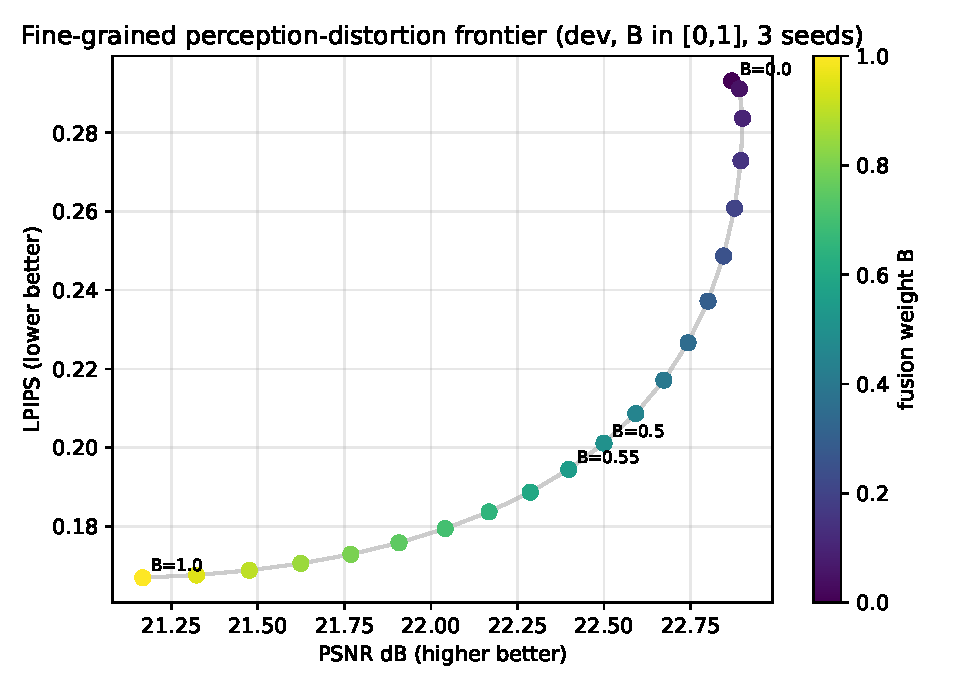
\includegraphics[width=0.85\linewidth]{B_CURVE.pdf}
\caption{The dense 21-point sweep of the dial: LPIPS strictly monotone from $0.293$ to $0.167$; PSNR declines from $22.87$ to $21.17$ dB with one shallow interior maximum ($+0.03$ dB at $B=0.10$).}
\end{figure}

\subsection*{C.5 Robustness studies in full}


The locked claim of main §4 fixes one operating point: the balanced dial $B$, at a single $5.0\%$ operator, on one $64\times64$ resolution, under noiseless acquisition. This section asks how far that operating point reaches --- across sampling rate, across measurement noise, and across the image population. All results here are \textbf{development-level}: they reuse the frozen system, re-select nothing on the locked split, and constitute supplementary evidence rather than a second pre-specified claim. We label them as such throughout and treat none of them as certified. The measurement-consistency guarantee, however, is not development-level: because $A P_0 = 0$ holds for every operator by construction, $A\hat{x}_B = y$ remains exact at every rate and every noise level below.

\subsection*{C.6 Cross-rate generalization (development-level)}

To test whether the balanced-fusion advantage is specific to the $5\%$ operator, we reuse the rate-agnostic priors unchanged and retrain only the lightweight anchor refiner at $2\%$ ($m=82$) and $10\%$ ($m=410$), then run the identical pipeline: select the global scalar $B$ on validation under the same tolerance rule, and score on the held-out development split (3 seeds per rate). This does not re-touch the frozen $5\%$ locked result, which appears only as the anchor point.

The advantage holds at every rate. Balanced fusion lowers LPIPS relative to the VQAE branch by $-0.116$ ($29.3\%$) at $2\%$, $-0.098$ ($32.6\%$) at $5\%$, and $-0.076$ ($34.2\%$) at $10\%$, with all $3/3$ seeds agreeing in direction at each rate and a PSNR cost of $-0.39$, $-0.45$, and $-0.43$ dB respectively --- below the pre-specified $0.5$ dB validation tolerance throughout. The relative gain grows mildly with sampling rate: at higher rates more genuine detail is recoverable for the fusion to exploit, which is consistent with the fusion mechanism rather than an artifact of a single operator.

\textbf{Table C2. Cross-rate generalization (development-level, 3 seeds per rate).}

\begin{center}\begin{tabular}{lcccc}
\toprule
Sampling rate & $\Delta$LPIPS (balanced $-$ VQAE) & Relative gain & $\Delta$PSNR (dB) & Seeds same-direction \\
\midrule
$2\%$ ($m=82$) & $-0.116$ & $29.3\%$ & $-0.39$ & $3/3$ \\
$5\%$ ($m=205$, \textit{locked}) & $-0.098$ & $32.6\%$ & $-0.45$ & $3/3$ \\
$10\%$ ($m=410$) & $-0.076$ & $34.2\%$ & $-0.43$ & $3/3$ \\
\bottomrule
\end{tabular}\end{center}


\subsection*{C.7 Noise robustness (development-level)}

The locked result is noiseless. To probe robustness we add i.i.d. Gaussian noise of standard deviation $\sigma_\varepsilon$ to the bucket measurements and re-run the frozen system with the balanced $B$ unchanged (3 seeds, locked split). Two behaviors emerge. First, VQAE is the most noise-stable branch but always the least perceptual. Second, and more instructive, full VQGAN degrades sharply as noise grows --- its fine synthesized detail amplifies the measurement noise --- so that balanced fusion, which the noiseless ladder places \textit{above} full VQGAN, \textbf{overtakes it at $\sigma_\varepsilon = 0.02$} (LPIPS $0.197$ for balanced versus $0.204$ for full VQGAN) and beats it decisively at $\sigma_\varepsilon = 0.05$ ($0.250$ versus $0.293$).

\textbf{Table C3. Noise robustness, LPIPS by bucket-noise level (development-level, 3 seeds, locked split, $B$ frozen).}

\begin{center}\begin{tabular}{lccc}
\toprule
Bucket noise $\sigma_\varepsilon$ & VQAE & Balanced & Full VQGAN \\
\midrule
$0.000$ & $0.300$ & $0.202$ & $0.172$ \\
$0.005$ & $0.299$ & $0.199$ & $0.172$ \\
$0.010$ & $0.297$ & $0.195$ & $0.176$ \\
$0.020$ & $0.295$ & $0.197$ & $0.204$ \\
$0.050$ & $0.304$ & $0.250$ & $0.293$ \\
\bottomrule
\end{tabular}\end{center}


This is the behavior a controlled interior operating point should have: balanced fusion keeps most of VQGAN's perceptual benefit at low noise while degrading far more gracefully as the measurement becomes unreliable. The crossover is not evidence that noise certifies anything about the null space --- the guarantee $A\hat{x}_B = y$ concerns only the row space at every $\sigma_\varepsilon$ --- but it does show that the recommended dial position is also the robust one.

\subsection*{C.8 Breadth of improvement and its failure mode}

The gain is broad, not anecdotal. Balanced fusion improves LPIPS on $99.0\%$, $97.5\%$, and $99.2\%$ of locked images for the three seeds respectively, worsening it on at most $13$ of $512$ images, with a worst-case regression of only $+0.07$ LPIPS and most regressions far smaller. The failures are not random: they concentrate on \textbf{man-made periodic and edge structure} --- fences, vehicle body panels, airplane fuselages --- where the natural-image VQGAN prior is a mismatch and synthesizes texture that conflicts with the regular geometry the scene actually contains. This is the expected and interpretable failure mode of a natural-image prior applied to structured man-made content, and it delimits where the dial should be advanced with care: the reach of responsible injection is bounded by the support of the prior, not by the measurement.

\begin{figure}[H]\centering
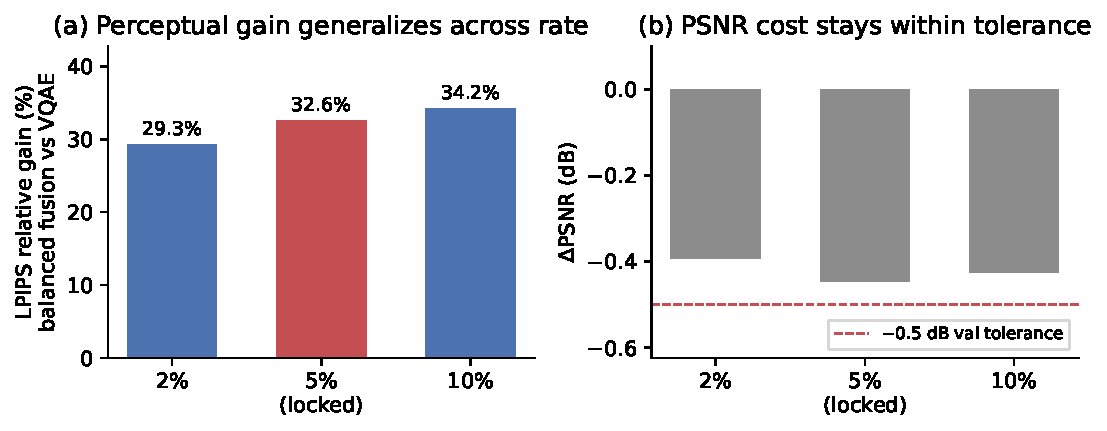
\includegraphics[width=0.85\linewidth]{rate_generalization_figure.pdf}
\caption{Cross-rate generalization (development-level): the balanced dial's relative LPIPS gain at 2\%, 5\% (locked), and 10\% sampling.}
\end{figure}

\begin{figure}[H]\centering
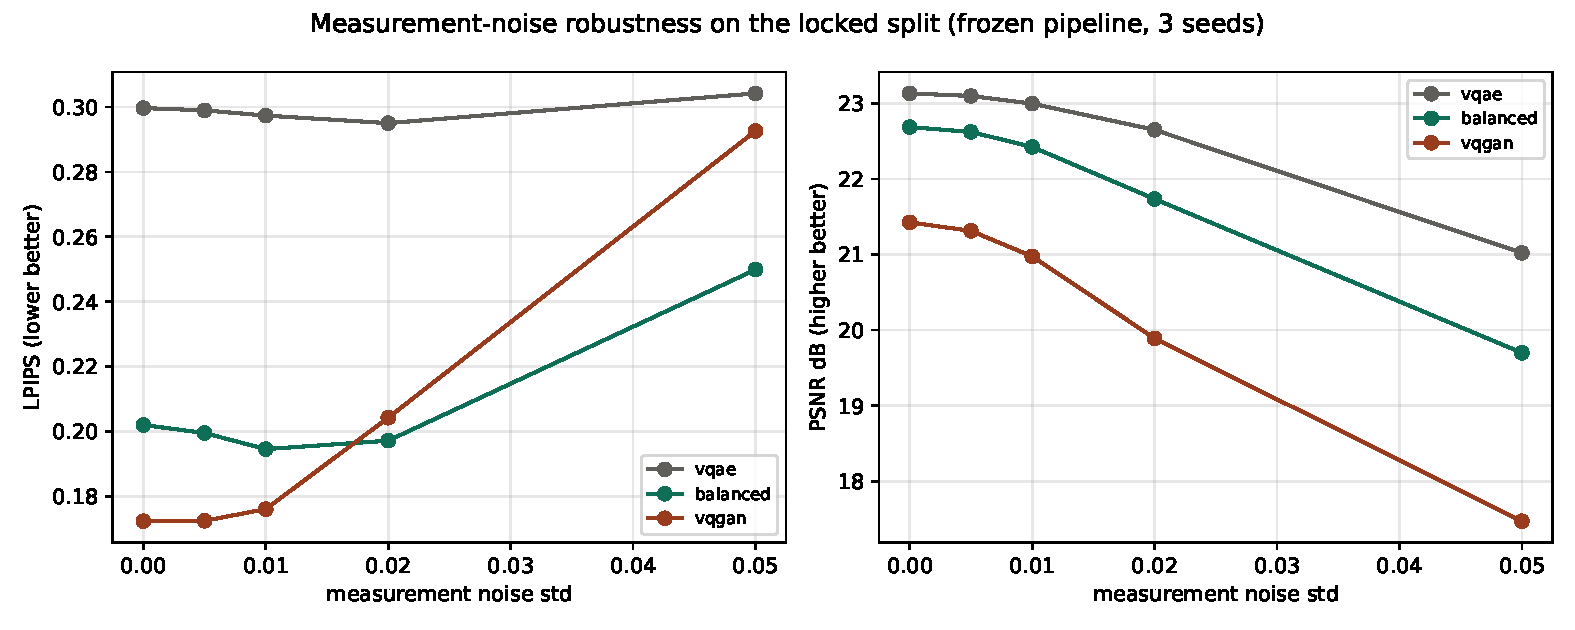
\includegraphics[width=0.85\linewidth]{NOISE_ROBUSTNESS.pdf}
\caption{Noise robustness (development-level): balanced fusion degrades gracefully and overtakes full VQGAN at $\sigma_\varepsilon = 0.02$.}
\end{figure}

\section*{Appendix D. Extended related work}

Our work sits at the intersection of computational ghost imaging, the range--null geometry of undersampled linear inverse problems, generative image priors, and the recent literature on hallucination, fundamental limits, and trustworthy reconstruction. What organizes the discussion below is a single distinction: almost every prior line uses the range--null decomposition, or a prior over the unmeasured content, to \textbf{reconstruct} --- to produce one image that looks right or scores well. We instead use the same geometry to \textbf{certify, bound, and meter}: to prove what the bucket measurement can and cannot vouch for, to audit that accountability at test time without ground truth, and to inject admittedly invented detail only where the measurement is provably blind. Each subsection first summarizes the line, then states our delta.

\subsection*{D.1 Ghost imaging and single-pixel imaging}

Ghost imaging originated as a quantum-optical curiosity: Pittman et al. (1995) recovered a magnified aperture image purely from photon-coincidence correlations, with no image present in either detector's individual counts. Gatti et al. (2004) then proved analytically that classically correlated thermal beams reproduce all the imaging features of entangled ghost imaging, and Ferri et al. (2005) demonstrated both ghost image and ghost diffraction from a single classical thermal source by altering only the reference arm. Shapiro (2008) and Bromberg et al. (2009) collapsed the modality to its computational core: with the illumination patterns known, a single bucket detector suffices, so ghost imaging is classical coherence propagation and the reconstruction is a correlation $C(\rho) = \sum_m \phi_m(\rho)\, y[m]$ against known patterns --- precisely our forward operator $y = Ax$. In parallel, the single-pixel camera (Duarte et al., 2008) and compressive ghost imaging (Katz et al., 2009) established the undersampled regime $y = \Phi x$ with $m \ll n$, recovered by $\ell_1$/TV minimization, and stated the governing fact plainly: since $m < n$, infinitely many images satisfy the same measurements, and recovery is possible only under a prior. Gibson et al. (2020) survey this progression from correlation through compressed sensing to learned reconstruction; Song et al. (2025) update it and flag interpretability and generalization as unresolved.

\textbf{Our delta.} These works establish the physical instantiation of our operator $A$ and the undersampled regime that makes its null space non-trivial. We take the "infinitely many $x$ satisfy the same $y$" observation --- usually stated in passing to motivate a sparsity prior --- and elevate it into the load-bearing object of the paper: a constructive, per-instance feasible-but-wrong witness and a test-time certificate over exactly this measurement model.

Learned ghost-imaging reconstructors sharpen the stakes. Lyu et al. (2017) restored recognizable images at sampling ratios as low as $\beta = 0.05$, where compressed sensing collapses, and candidly noted the outputs "do not resemble exactly the ground truth"; the CNN pipeline of He et al. (2018) and the U-Net denoiser of Shimobaba et al. (2018) buy large PSNR/SSIM gains with no enforced measurement consistency; and the X-ray study of Huang et al. (2024) argues rigorously that reducing the number of measurements does not itself add information, so any sub-sampling-limit detail a learned reconstructor supplies originates from the prior, not the measurement.

\textbf{Our delta.} This GI-native line is the empirical hook for our converse: at low $\beta$ the network fills the null space with trained-in structure the measurement cannot certify. Prior work optimizes quality (MSE, recognizability, PSNR); we separate quality from accountability, audit the learned reconstructor alongside classical ones, and never claim the bucket certifies the invented texture.

For breadth of the modality itself we point the reader to Edgar, Gibson \& Padgett's (2019) survey of single-pixel imaging, whose operator abstraction is the one this paper audits.

\subsection*{D.2 Range--null and data-consistency reconstruction}

A large body of work exploits the range--null decomposition $x = P_R x + P_0 x$ with $P_R = A^\dagger A$, $P_0 = I - A^\dagger A$, and $A P_0 = 0$. The classical antecedents of "edit freely, keep the measurement exact" are the alternating-projection extrapolators --- Gerchberg (1974) and Papoulis (1975) for band-limited completion, generalized by Youla \& Webb (1982) --- which already alternate a prior step with a hard projection onto $\{Hx = y\}$. Its modern deep-learning-era formulation is IDBP (Tirer \& Giryes, 2018), which alternates denoising with a backward projection so that all restoration dynamics live strictly in the null space. Schwab et al. (2019) formalized the null-space network $L = \mathrm{Id} + (\mathrm{Id} - A^+A)N$, proving it is a convergent regularization that edits only $\ker(A)$ while preserving data consistency exactly, and Chen \& Davies (2020) trained separate range- and null-space networks over the same $P_R = H^\dagger H$, $P_0 = I - H^\dagger H$ split. In imaging practice, hard data-consistency layers (Schlemper et al., 2018), model-based unrolling with an explicit $(A^H A + \lambda I)^{-1}$ solve (Aggarwal et al., 2019), variational networks (Hammernik et al., 2018), learned primal--dual (Adler \& Öktem, 2018), ADMM-Net (Yang et al., 2016), and ISTA-Net (Zhang \& Ghanem, 2018) all restore or preserve the measured component while a learned prior supplies the rest. The same construction anchors the most recent null-space methods: RND-SCI (Wang et al., 2023) reconstructs hyperspectral snapshots as $x = \Phi^\dagger y + (I - \Phi^\dagger \Phi)q$ with a conditional network generating only the null term; NPN (Jacome et al., 2025) trains a network to predict a low-dimensional null-space projection $Sx^*$ from $y$, explicitly noting that data fidelity leaves the null space uncontrolled; and GSNR (Gualdron-Hurtado et al., 2026) builds a graph-smooth basis for $\mathrm{Null}(H)$ via the null-restricted Laplacian $T = P_n L P_n$ and proves minimax coverage/predictability bounds for the invisible directions, gaining up to 4.3 dB.

\textbf{Our delta --- the null-space reconstruction cluster (position against).} This cluster is our closest prior art and our sharpest point of departure. Every one of these methods uses $A P_0 = 0$ to install the \textit{correct} content in the null space, and treats consistency-by-construction as a fidelity virtue --- a proxy for correctness. RND-SCI generates a monolithic null term for speed and PSNR; NPN and GSNR go further and argue the null content \textit{is} predictable, learning it from $y$ and enforcing only soft fidelity, with GSNR's coverage/predictability curves computed at design time from dataset statistics. We invert the entire premise. The same $A P_0 = 0$ that lets these methods edit the null space without breaking consistency is exactly why measurement consistency \textbf{cannot certify} what they put there. We contribute (i) a constructive feasible-but-wrong witness, matching the record to machine precision, showing the construction is a barrier rather than a guarantee; (ii) a ground-truth-free, test-time certificate that contracts each measured mode by exactly $\lambda/(\lambda+\sigma_i^2)$, a closed-form modal spectrum rather than a soft penalty or a design-time diagnostic; and (iii) an exact-consistency dial that keeps $A\hat{x}_B = y$ for \textbf{every} setting $B$ behind a pre-specified locked gate. Schwab et al. (2019), Chen \& Davies (2020), and IDBP (Tirer \& Giryes, 2018) supply the theoretical scaffolding we build on, but none poses a converse, audits accountability, or meters the invention.

Plug-and-play priors (Venkatakrishnan et al., 2013) and Regularization by Denoising (Romano et al., 2017) decouple a forward-model solve from a black-box denoiser prior, the conceptual ancestor of separating measured fidelity from supplied content.

\textbf{Our delta.} PnP and RED let the denoiser alter measured modes too and offer no test-time measurement-accountability certificate; our injection is confined to the null space so $A\hat{x}_B = y$ holds exactly, and our audit reads the per-mode contraction regardless of which prior is plugged in.

\subsection*{D.3 Generative and VQ priors for inverse problems}

Generative priors replace sparsity with a learned low-dimensional manifold. Bora et al. (2017) showed $O(k \log L)$ measurements suffice to recover signals near a generative model's range under the Set-Restricted Eigenvalue Condition --- a condition that requires differences of natural signals to lie \textit{away} from $\mathrm{null}(A)$. Shah \& Hegde (2018) give a projected-gradient GAN-prior solver with linear-convergence guarantees under the same S-REC; Asim et al. (2020) use invertible (flow) priors with zero representation error and prove recovery error is governed by the smallest $n-m$ singular values; Lunz et al. (2018) learn an adversarial regularizer that approximates distance to the data manifold; and Yeh et al. (2017) hallucinate plausible content strictly inside a missing region while pinning observed pixels. Untrained priors --- Deep Image Prior (Ulyanov et al., 2018) and the Deep Decoder (Heckel \& Hand, 2019) --- show that architecture alone supplies image statistics, with the Deep Decoder making the reachable set an explicit capacity knob. The vector-quantized line runs from VQ-VAE (van den Oord et al., 2017) through VQ-VAE-2 (Razavi et al., 2019), which factorizes an image into a global-structure code and a local-detail code, to VQGAN (Esser et al., 2021), whose patch discriminator synthesizes crisp texture that plain VQ-VAE cannot recover. Codebook priors dominate blind face restoration --- VQFR (Gu et al., 2022), CodeFormer (Zhou et al., 2022), and RestoreFormer (Wang et al., 2022) --- with CodeFormer exposing a single scalar $w \in [0,1]$ that trades fidelity for quality at test time.

\textbf{Our delta.} We build our supply mechanism directly on this lineage: VQ-VAE-2's structure/detail factorization motivates our structure (VQAE) plus detail (VQGAN) split, and CodeFormer's scalar $w$ is the closest interface to our dial $B$. But every one of these controls acts on \textit{entangled} features, so higher quality genuinely costs measurement fidelity ($A\hat{x} \neq y$), and S-REC-style guarantees explicitly assume away the regime --- null-space differences that are uncontrolled --- where we operate. Our dial injects the same VQ-generated content \textbf{only} in $P_0$, so $A\hat{x}_B = y$ holds exactly for every $B$, and we treat the resulting texture, however realistic, as content the measurement provably cannot certify. Asim et al.'s (2020) smallest-$(n-m)$ singular-value bound is the quantitative cousin of our per-mode $\lambda/(\lambda+\sigma_i^2)$ contraction; we make that spectrum exact and auditable.

\subsection*{D.4 Perception--distortion tradeoffs and perceptual metrics}

Blau \& Michaeli (2018) proved a fundamental, distortion-measure-agnostic perception--distortion tradeoff: lowering distortion forces the reconstruction distribution away from natural-image statistics, so "matches the reference" and "looks real" are formally at odds; their rate-distortion-perception extension (2019) adds that perceptual realism must be paid for in rate or distortion. SRGAN (Ledig et al., 2017), ESRGAN (Wang et al., 2018) with its scalar network-interpolation dial, and the PIRM challenge (Blau et al., 2018) operationalized this plane for super-resolution, and LPIPS (Zhang et al., 2018) became the standard perceptual metric --- the one we use to report our locked improvement. PULSE (Menon et al., 2020) is the canonical exhibit that consistency is not correctness in super-resolution: visually distinct realistic faces all downscale to the identical low-resolution input.

\textbf{Our delta (position against).} Blau \& Michaeli's tradeoff is \textit{statistical} --- a divergence between the reconstruction distribution and natural-image statistics --- and its GAN Lagrange knob is the conceptual ancestor of our dial. Our converse is \textit{geometric and exact}: feasible-but-wrong images matching $y$ to machine precision make the null content unverifiable regardless of any distributional statistics. ESRGAN's $\alpha$ and CodeFormer's $w$ trade quality for fidelity along a soft curve; our dial is null-space-confined, so the measurement stays exact at every point rather than at one tradeoff position. We use LPIPS to quantify the perceptual win and keep it strictly on the quality ledger, never conflating it with accountability. PULSE supplies feasible-but-wrong images but presents one as "the" answer and audits nothing; we govern and certify.

\subsection*{D.5 Diffusion inverse-problem solvers}

Modern training-free solvers use a pretrained diffusion model as a prior. The score-SDE framework (Song et al., 2021) conditions an unconditional model on the observation; Song et al. (2022) factor the operator as $A = P(\Lambda)T$ and keep measured transform coefficients while synthesizing the rest; DDRM (Kawar et al., 2022) diffuses in the SVD spectral space, synthesizing zero-singular-value (null) directions and conditioning measured ones with a per-mode blend weight; MCG (Chung et al., 2022) writes $A = I - P^\top P$ (our $P_0$) to update only the orthogonal complement while pinning the measured subspace; DPS (Chung et al., 2023) adds a soft measurement-gradient step for general noisy problems; and DiffPIR (Zhu et al., 2023) embeds half-quadratic-splitting into the sampling loop. DDNM (Wang et al., 2023) is the most direct methodological cousin of our dial: it fixes the range to $A^\dagger y$ and lets a diffusion model synthesize only the null-space content $(I - A^\dagger A) \bar{x}$, so $A\hat{x} = y$ holds exactly. The survey of Daras et al. (2024) taxonomizes the field and gives the canonical noiseless data-consistency update $(I - A^\dagger A)\, \mathbb{E}[X_0 \mid x_t] + A^\dagger y$.

\textbf{Our delta.} DDRM's per-singular-value treatment and DDNM's exact null-space fill are the spectral and structural skeletons of our framework, and MCG's $A = I - P^\top P$ is literally our $P_0$. The difference is direction and purpose. DPS, DiffPIR, DDRM ($\eta_b < 1$), and the score-based solvers enforce consistency softly, so $A\hat{x} \neq y$ in general and prior content leaks into measured modes; DDNM and MCG keep the null-space move exact but chase SOTA restoration realism. We do not compete on restoration quality and do not claim to beat diffusion. Instead, our certificate is a ground-truth-free \textit{audit} --- not a sampler --- that quantifies, per measured mode, how much of any such solver's output the measurement can vouch for; and our dial governs the null-space content these methods fill ungoverned, with an exact-consistency guarantee and a locked gate they do not provide.

\subsection*{D.6 Hallucination, instability, and fundamental limits}

A sobering literature documents that consistency and visual quality decouple from correctness. Antun et al. (2020) showed state-of-the-art learned MRI/CT reconstructors are unstable to near-invisible perturbations and can erase small structural detail while stable compressed-sensing baselines are not; Genzel et al. (2020) offered the balancing counterpoint that, under matched adversarial testing, standard networks match a robust TV benchmark and much instability traces to noiseless-training "inverse crimes." Buğday et al. (2026) inserted diagnostically misleading anatomical hallucinations via imperceptible k-space perturbations that PSNR/NRMSE/SSIM cannot detect. Bhadra et al. (2021) formalized hallucinations by projecting a reconstruction onto measurement and null spaces, showing null-space hallucinations are attributable solely to the prior and cannot be assessed without the ground truth; Gottschling et al. (2025) prove kernel-aware no-free-lunch theorems and construct explicit kernel-element perturbations that destabilize learned maps --- the nearest formal ancestors of our witnesses, which differ in kind (cross-class semantic splices on the governed dial's own operator, matching the record tighter than the noisy truth) but not in geometry; DynamicDPS (Kim et al., 2025a) adopts the same intrinsic (data-inconsistent) versus extrinsic (null-space) split and suppresses both with a diffusion prior plus data consistency; and HalluGen (Kim et al., 2025b) fabricates controllable hallucinations by gradient ascent to train reference-free detectors, noting that consistency-preserving errors are the hardest to catch. Learned primal--dual (Adler \& Öktem, 2018) even internally observes that a true feature is indistinguishable from a false feature of the same size and contrast. The fundamental-limits side is anchored by Iagaru et al. (2026), who prove necessary-and-sufficient conditions for detail-transfer hallucination in (possibly nonlinear) inverse problems --- consistent decoders can only hallucinate details that are almost invisible in measurement space ($\lVert f(x + x_{\det}) - f(x)\rVert \le 2\epsilon$) --- and give ground-truth-free, forward-model-only algorithms that bound and assess hallucination magnitude via feasible-set diameters (worst-case kernel size).

\textbf{Our delta --- the limits-and-assessment line (position against).} This is the line we must not overclaim against, and we cite it as the anchor for the barrier itself. Antun et al. (2020), Buğday et al. (2026), and Bhadra et al. (2021) establish empirically and by SVD decomposition that consistency and quality metrics do not certify correctness; Iagaru et al. (2026) prove the fundamental limit and occupy the generic slot of forward-model-only, ground-truth-free hallucination \textit{assessment}. We do not claim "null content is unverifiable" or "ground-truth-free assessment" as novel --- that ground is theirs. Our contribution is on four axes they do not cover. First, where Iagaru et al. give feasible-set-diameter \textit{bounds} (a sup over feasible sets, requiring paired data), we give an \textbf{exact} per-mode contraction $\lambda/(\lambda+\sigma_i^2)$ from the operator's SVD, applied as a test-time plug-in audit across BP, Tikhonov, CS-TV, and learned reconstructors. Second, where they establish \textit{existence} via necessary-and-sufficient conditions, we give a \textbf{constructive} per-instance feasible-but-wrong witness that matches the record to machine precision. Third, we frame and demonstrate a \textbf{quality-versus-accountability separation} (PSNR essentially flat while measurement residuals drop orders of magnitude) as an explicit protocol. Fourth, and entirely uncontested, we move from \textit{assessment} to \textit{governance}: a constructive, metered null-space injection dial with $A\hat{x}_B = y$ exact for every $B$ and a pre-specified locked gate. The clean axis is assessment versus governance, exact versus bound, constructive versus existential. Bhadra et al.'s (2021) null-space hallucination map requires the ground truth --- exactly the quantity our converse proves unverifiable --- so we cite it to say the null-space error is real but cannot be certified at test time.

\subsection*{D.7 Uncertainty, conformal prediction, and trust}

The standard response to unreliable reconstruction is uncertainty quantification. Kendall \& Gal (2017) established the aleatoric/epistemic taxonomy; Narnhofer et al. (2021) produce Bayesian epistemic-uncertainty maps for variational MRI. On the distribution-free side, Angelopoulos et al. (2022) endow any image-to-image regressor with per-pixel risk-controlling prediction intervals to flag hallucinations, conformal risk control (Angelopoulos et al., 2022) guarantees $\mathbb{E}[\mathrm{loss}] \le \alpha$ for bounded monotone losses, Wen et al. (2024) conformalize the downstream task output rather than per-pixel maps, and Lu et al. (2022) apply ordinal conformal sets to disease severity rating. Wen et al. (2024) in particular argue, as we do, that per-pixel uncertainty maps are the wrong object because they miss many-pixel hallucinated structure.

\textbf{Our delta.} These guarantees are either heuristic (Bayesian std maps) or ground-truth-dependent at calibration (RCPS, conformal risk control, task-conformal), and they operate in output/pixel/label space. Our certificate is deterministic, ground-truth-free at test time, and lives in the operator's spectral geometry: it contracts each \textit{measured} mode by exactly $\lambda/(\lambda+\sigma_i^2)$ and audits measurement accountability rather than pixel error or a labeled risk. Crucially, using Kendall \& Gal's own taxonomy, our accountability is neither aleatoric nor epistemic --- it is a third, geometry-determined quantity: null-space unverifiability persists even with a perfect model in the noiseless limit, because $A P_0 = 0$ makes null content invisible to $y$ regardless of noise or model confidence. No calibration set can fix what the converse proves.

\subsection*{D.8 Cross-field framings: identifiability, information theory, and Bayesian inversion}

Our thesis has deep provenance outside imaging. Econometric identification theory (Koopmans \& Reiersøl, 1950) established that observationally equivalent structures generate the identical distribution, so a characteristic is knowable only if invariant across all such structures --- identification precedes estimation. Rothenberg (1971) tied local identifiability to nonsingularity of the Fisher information matrix, making non-identifiability a rank deficiency / null space in information geometry. Manski (2003) founded partial identification --- when data do not point-identify a parameter they confine it to a sharp set, and honest inference reports that set --- and Lewbel (2019) formalized set identification and \textit{normalizations}: restrictions that select within the identified set without altering any meaningful quantity. On the imaging side, Landau (1967) fixed the sampling-density threshold below which degrees of freedom exceed measurements and a non-trivial null space is forced by necessity, Candès, Romberg \& Tao (2004) proved exact CS recovery under sparsity while noting that without the prior distinct signals share identical partial measurements, and Stuart (2010) cast inverse problems as Bayesian posteriors in which, when data dimension is below the unknown, the prior remains decisive even in the zero-noise limit. Within the imaging sciences proper the lineage is older and more direct: Backus \& Gilbert (1968--1970) characterized exactly which linear functionals of an underdetermined model are resolved by finite data --- a functional is determined iff its representer lies in the row space, our certifiable/uncertifiable split for linear observables --- and Barrett \& Myers (\textit{Foundations of Image Science}, 2004) built the estimability and null-function calculus, and task-based image-quality assessment, on the identical range/null decomposition. MacKay (1992) is the Bayesian antecedent of the certificate itself: his effective number of well-determined parameters $\gamma = \sum_i \lambda_i/(\lambda_i+\alpha)$ sums our per-mode contraction over the spectrum (main §3.2).

\textbf{Our delta.} These fields supply the rigorous vocabulary we import and instantiate, and we own the lineage rather than reinvent it. Our feasible-but-wrong images are the imaging analogue of Koopmans \& Reiersøl's observational equivalence and Rothenberg's singular information direction; our null space $P_0 = I - A^\dagger A$ is Manski's identification region, Landau's forced kernel, and Barrett \& Myers's null-function subspace; our certifiable-functional split is Backus--Gilbert resolvability; and, most sharply, our governed dial is Lewbel's \textit{normalization} --- injecting null content is "without loss of generality" for the measurement, since $A\hat{x}_B = y$ exactly for every $B$, leaving the identified quantity untouched. Candès--Romberg--Tao's converse is the CS-side twin of the econometric one, and Stuart's "prior stays decisive" is the Bayesian mirror of our per-mode contraction, whose factor $\lambda/(\lambda+\sigma_i^2)$ is exactly a Gaussian-posterior variance reduction along each singular direction --- the same term MacKay aggregates into $\gamma$, which we instead read per record as a test-time audit. Our contribution is not a new scalar on $(A,\sigma)$: on the linear-Gaussian layer these objects are settled, and any quantity defined there is a renaming of one of them. It is the \textit{constructive converse}, the repurposing of the modal contraction as a ground-truth-free per-record certificate that separates quality from accountability, and the governed injection dial --- an operational stack, unified for undersampled ghost imaging, that these prior framings describe in pieces but never assemble as a governance instrument. The \textbf{no-adaptation lemma} (main §4.5) is, as mathematics, an elementary measurability fact; we state it formally because the reconstruction literature repeatedly proposes per-image adaptation schemes that cannot, even in principle, out-adapt their own global prior on a fixed record --- and because its value lies in the pairing with the empirical finding that the $y$-predictable remainder is worth essentially nothing here.

\subsection*{D.9 Novelty statement}

Every line above uses the range--null geometry, or a prior over the unmeasured content, to \textbf{reconstruct}: install the "correct" prior in the null space for fidelity (Wang et al., 2023 AAAI; RND-SCI; DDNM; MCG), learn to predict null content from $y$ (NPN; GSNR; Chen \& Davies, 2020), fabricate null-like error to benchmark detectors (HalluGen), quantify output uncertainty against calibration data (RCPS; conformal risk control; Wen et al., 2024), or prove abstractly that the kernel forces hallucination (Iagaru et al., 2026; Bhadra et al., 2021; Antun et al., 2020). We use the identical geometry to \textbf{certify, bound, and meter}, and our contribution rests on four operational differences. \textbf{First}, we make the barrier \textit{constructive}: an explicit feasible-but-wrong witness that matches the same bucket record to machine precision --- tighter than the noisy truth --- turning "consistency is not correctness" from a theorem about maps (Iagaru et al., 2026) and an SVD diagnostic (Bhadra et al., 2021) into a per-instance object --- and where Gottschling et al.'s (2025) kernel constructions establish destabilizing existence, ours are cross-class, record-tight, and displayed.

\textbf{Second}, we give a ground-truth-free, reconstructor-agnostic \textbf{test-time certificate} that contracts each measured mode by \textit{exactly} $\lambda/(\lambda+\sigma_i^2)$ --- a closed-form modal spectrum, not a feasible-set-diameter bound (Iagaru et al., 2026), a soft penalty (NPN; GSNR), a design-time predictability curve (GSNR), or a calibrated statistical interval (Angelopoulos et al., 2022) --- auditing BP, Tikhonov, CS-TV, and learned reconstructors uniformly --- including, in main §5, three \textit{published} DL-GI pipelines decomposed on their own released or measured operators --- and \textbf{separating image quality from measurement accountability}.

\textbf{Third}, that separation is demonstrated as an explicit protocol (perceptual/PSNR quality essentially unchanged while measurement residuals fall orders of magnitude), an axis none of the reconstruction or UQ lines report.

\textbf{Fourth}, we convert null-space injection from an all-or-nothing fill into a single-scalar, pre-specified \textbf{governed dial} that fuses VQAE structure and VQGAN detail and keeps $A\hat{x}_B = y$ \textit{exact} for every $B$ behind a locked gate --- moving the field from \textit{assessment} (does a reconstruction hallucinate?) to \textit{governance} (how much invented detail do we add, where the bucket is provably blind, without ever breaking the measurement or reporting the addition as measured evidence?).

We explicitly do \textbf{not} claim SOTA, do not beat diffusion, and never claim the measurement certifies invented texture --- the point is that it provably cannot. That inversion --- \textbf{reconstruct, becomes certify / bound / meter} --- is the slot this paper occupies.

\medskip\hrule\medskip

\section*{Appendix E. Projector forensics: full decompositions}

\textbf{Table E1. Forensics summary (own operator, own code).}

\begin{center}\begin{tabular}{lccc}
\toprule
Pipeline & Headline vs own range ceiling & Gain split row/null & Terminal null share \\
\midrule
PEDL (fine-tuned) & $25.1$ vs $17.0$ dB ($+8.1$) & $61/39$ & $96.9\%$ \\
GIDC (untrained; known-GT scene) & $19.5$ vs $15.0$ dB ($+4.5$) & $60/40$ & $95.4\%$ \\
Noise2Ghost (self-supervised) & $18.4$ vs $15.3$ dB ($+3.1$) & $5/95$ & $92.7\%$ \\
\bottomrule
\end{tabular}\end{center}

\textbf{Audit on the measured operator [development-level].} Running $\Pi_y^\lambda$ ($\lambda = 10^{-6}$) on GIDC's measured speckle operator against the substituted-GT reconstruction: RelMeasErr $3.04\times10^{-3} \to 2.96\times10^{-15}$, PSNR $19.54 \to 19.74$ dB, max deviation of the measured modal contraction from $\lambda/(\lambda+\sigma_i^2)$: $3.5\times10^{-11}$ (float64; $\sigma_i \in [511, 26607]$). Artifact: \texttt{gidc\_measured\_audit.json}.

\textbf{Table E2. Reproducibility of the audits.}

\begin{center}\begin{tabular}{lccccc}
\toprule
Pipeline & Code source & Operator source & GT status & Audit & Key caveat \\
\midrule
PEDL & released (TF1, run unmodified) & released learned patterns & known (sim) & full error attribution & final consistency $2.3\times10^{-2}$ \\
GIDC & released (TF1, run unmodified) & measured speckle (data.mat) & experimental: none; substituted known-GT scene & content split; error split on substituted scene & operator calibration inherited \\
Noise2Ghost & released (pip package; call-level adaptations disclosed) & released sim masks & known + noisy record & full error attribution & record noise $1.2\times10^{-2}$ \\
\bottomrule
\end{tabular}\end{center}


\subsection*{E.1 External validity: projector forensics of published pipelines, on their own operators}

Everything above is demonstrated on our operator. To test whether the two-ledger reading describes the field rather than our construction, we audited three published DL-GI pipelines --- three different learning paradigms on three different operators --- using \textbf{each paper's own released or measured operator and each paper's own code}, with exact orthogonal attribution $\|\hat{x}-x\|^2 = \|P_R(\hat{x}-x)\|^2 + \|P_0(\hat{x}-x)\|^2$ computed from the SVD of \textit{their} $A$ (main-text Figure 8).


\textbf{Physics-enhanced deep learning SPI} (Wang et al. 2022a, \textit{Photon. Res.}; pretrained U-Net + measurement-loss fine-tuning; released learned patterns verified against their shipped record to $1.2\times10^{-7}$). Their fine-tuning trajectory, decomposed per step, is a two-phase object: of the $+4.36$ dB the 300 steps buy, $61.4\%$ of the MSE improvement is row-space repair --- exactly what a measurement loss is entitled to fix --- and $38.6\%$ is null-space spillover through the network's coupling. By step ${\sim}200$ the row ledger is exhausted ($96.9\%$ of the remaining error is null) and PSNR plateaus. The final $25.12$ dB stands $8.1$ dB above the operator's range ceiling of $16.99$ dB: everything above the ceiling is prior-supplied null content, truth-aligned on the audited scene (alignment ${\approx}0.85$) but, by the converse, unverifiable from the record.

\textbf{GIDC} (Wang et al. 2022b, \textit{Light Sci. Appl.}; untrained DIP-style network; $410$ \textit{physically measured} speckle patterns and photon-count buckets). On the experimental scene (no ground truth), $43.8\%$ of the published reconstruction's centered structure lies in the null space of the patterns actually measured --- a precise ledger location for the paper's far-field super-resolution claim, since the diffraction-limited speckle bounds the measured subspace and super-resolved content is definitionally null-space content. With a known scene substituted onto the same real patterns at their photon level (their code byte-identical), the gain attribution is $60.3\%$ row / $39.7\%$ null --- nearly identical to the fine-tuned pipeline's split --- with the untrained prior's null content genuinely moving toward the truth (alignment $0.07 \to 0.65$: GIDC's real merit, quantified), terminating $4.5$ dB above the ceiling at $95.4\%$-null residual error.

\textbf{Noise2Ghost} (Manni et al., 2025; self-supervised, and the one genuinely \textit{noisy} record, $\mathrm{rel}\,\varepsilon = 1.2\times10^{-2}$ --- the regime where range saturation is non-tautological because in-range denoising is possible). It is real: N2G's row-space error lands $42\%$ \textit{below} the noisy pseudo-inverse, an effect noiseless simulations cannot exhibit. And it is small: in-range denoising accounts for ${\approx}4.9\%$ of the total MSE improvement; $95.1\%$ is null-ledger (null error halved at alignment $+0.44$), with the terminal error $92.7\%$ null.


\textbf{The cross-target regularity, with its base rates.} The \textit{qualitative direction} of these findings is forced by the sampling rate and must be said plainly: at $6$--$25\%$ sampling, most of any scene's energy is null-space energy to begin with (the true scene carries $10.1\%$ of its energy in the learned operator's null space, $17.2\%$ in GIDC's, and the pseudo-inverse reference point has a $100\%$-null terminal error by construction), so "most residual error is null" is partially dimension counting.

What is \textit{not} forced, and constitutes the findings, are the quantitative splits and their agreement: the $61/39$ and $60/40$ row/null attributions of two entirely different optimizations, the $5/95$ split of the self-supervised method whose in-range denoising is real ($42\%$ below the noisy pseudo-inverse) yet small, the truth-alignment trajectories ($0.07 \to 0.65$ for GIDC), and the fact that all three terminate with the row ledger \textit{repaired} --- the methods reduce the null share of error below the base rate, and stall exactly when the certifiable ledger is exhausted.

Two caveats bound the audit's own accountability: the GIDC null attribution inherits any calibration error in the released patterns (the operator is measured, not exact), and the attribution is stated relative to the min-norm reference. None of the three pipelines applies an exact consistency projection (residuals $2.3\times10^{-2}$, $0.134$, and noise-floor respectively), so the audit step of main §3 is available to each at zero cost.

We stress the reading: this is not an accusation of error --- the null content these methods supply is often substantially truth-aligned --- it is the \textit{location} of their gains in the two-ledger account, measured on their own instruments. The separation law of main §3.3 describes the field, not just our operator.

\subsection*{E.2 Accelerated MRI: masked-Fourier forensics on real fastMRI}

The three pipelines above are ghost-imaging-native. To test the two-ledger reading on a real, second-modality operator --- not our speckle construction, and not a simulation --- we ran the same decomposition on real NYU fastMRI knee $k$-space with the exact masked-Fourier operator $A = MF$ (single-coil emulated, $M$ the released undersampling mask), and on the \textbf{official} fastMRI single-coil U-Net (chans $= 256$, wired from the released state dict). The operator is exact, so no calibration error is inherited: the projector identities hold in float64 on the real $k$-space to $\sim\!10^{-17}$, and the ESC ground truth $\lvert\operatorname{crop}(\operatorname{ifft2c}(k))\rvert$ agrees to correlation $1.00000$. Because $A = MF$ is a masked Fourier operator, the zero-filled reconstruction \textit{equals} $P_R x_{\mathrm{gt}}$ exactly; its magnitude PSNR therefore \textbf{is} the range ceiling, with no SVD reference needed.

\textbf{The feasible-but-wrong witness carries over to real $k$-space.} Two different knees share one identical $R{=}8$ (nominal; effective $6.9\times$ after the autocalibration signal, ACS) undersampled record: a magnitude-legal $[0,1]$ POCS witness matches that record to median $2.5\times10^{-16}$ --- tighter than the clean truth matches its own noisy record --- while reading out at $20.3$ dB against the target, a visibly different knee. The converse of main §2 is not an artifact of our masks.

\begin{figure}[H]\centering
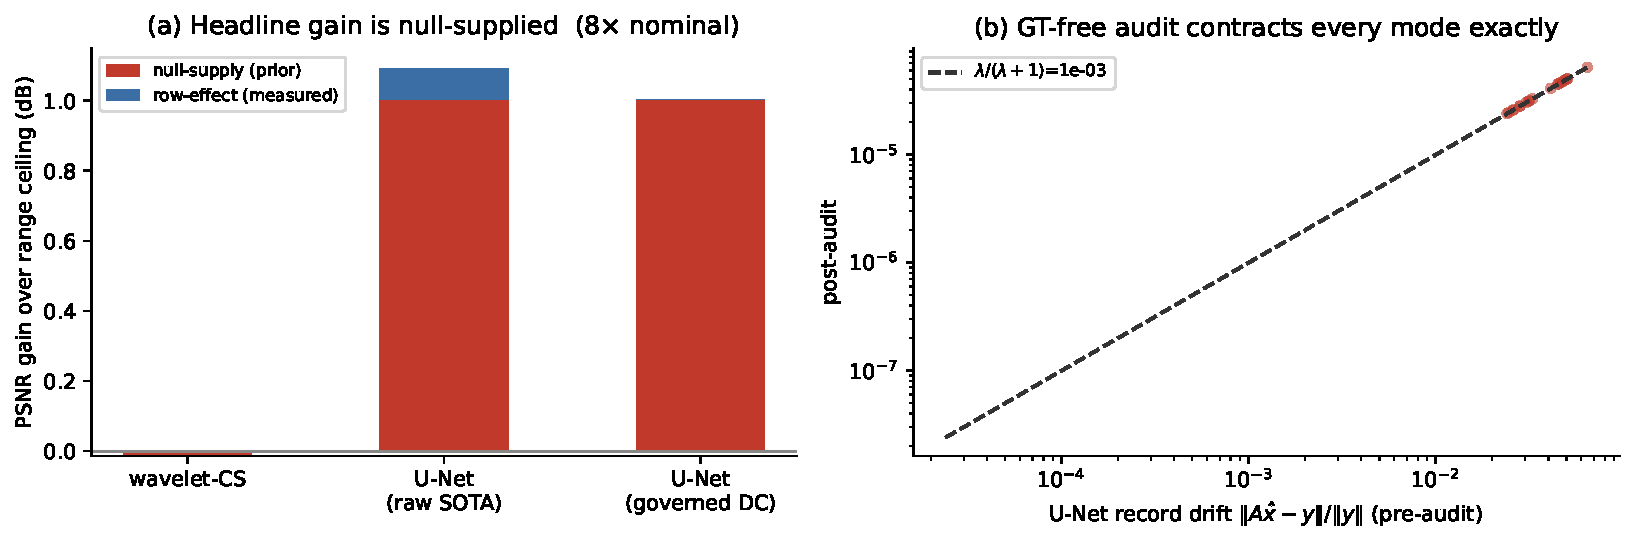
\includegraphics[width=1.0\linewidth]{FORENSICS_MRI_8x.pdf}
\caption{\textbf{The two ledgers on real fastMRI at $R{=}8$.} The official single-coil U-Net's $+1.09$ dB over the range ceiling is $92\%$ null-supplied; the zero-filled image \textit{is} $P_R x_{\mathrm{gt}}$, so the ceiling is exact, not a min-norm proxy. The governed data-consistent variant keeps the gain at exact record consistency.}
\end{figure}

\textbf{Table E3. fastMRI single-coil U-Net decomposition (real $k$-space, official state dict).} \textit{Ceiling} is the exact magnitude PSNR of $P_R x_{\mathrm{gt}}$ (zero-filled). \textit{U-Net drift} is the measured record inconsistency $\lVert A\hat{x}-y\rVert/\lVert y\rVert$. \textit{Governed DC} is $A^\dagger y + P_0 x_{\mathrm{UNet}}$; its own record drift is $\le 3.5\times10^{-16}$ at both rates (exact by construction).

\begin{center}\begin{tabular}{lcccccc}
\toprule
Rate (nom. / eff.) & Range ceiling & U-Net & Gain & Null share & U-Net drift & Governed DC \\
\midrule
$R{=}4$ / $3.7\times$ & $26.70$ dB & $29.68$ dB & $+2.98$ & $91\%$ & $5.9\%$ & $29.42$ dB \\
$R{=}8$ / $6.9\times$ & $24.32$ dB & $25.42$ dB & $+1.09$ & $92\%$ & $3.3\%$ & $25.33$ dB \\
\bottomrule
\end{tabular}\end{center}

The pattern of Appendix E.1 recurs on a modality that shares nothing with ghost imaging but the geometry: the U-Net's improvement over the ceiling is $91$--$92\%$ null-supplied, and the network is $3$--$6\%$ record-\textit{inconsistent} --- it moves the measured component off $A^\dagger y$. That inconsistency is the contingent content (a data-consistent estimator would have none): the governed variant $A^\dagger y + P_0 x_{\mathrm{UNet}}$ keeps nearly all the gain ($29.42$ vs $29.68$ dB at $R{=}4$) at exact record consistency (drift $3.5\times10^{-16}$), buying certifiability for $0.26$ dB.

\textbf{The GT-free audit contracts the drift by the closed-form factor.} Applied post-hoc to the data-inconsistent U-Net, the record-consistency audit $\Pi_y^\lambda$ contracts the measured drift by exactly $\lambda/(\lambda+1)$ --- median $5.86\times10^{-2}\to5.85\times10^{-5}$ at $\lambda=10^{-3}$ --- with per-mode deviation from the theoretical contraction $\le10^{-15}$. Masked-Fourier $A$ has a flat singular spectrum ($\sigma_i\equiv1$ on the sampled modes), so the modal contraction collapses to a single value; the non-uniform face of the same theorem appears in E.3.

\textbf{Certified-decision on real pathology boxes --- with the honest nuance.} On $429$ real fastMRI+ pathology bounding boxes, the ACS certifies the \textit{coarse} lesion but not the \textit{fine} detail. Full-box null-energy median is $13.5\%$ at $R{=}8$ and $18.4\%$ at $R{=}16$: the coarse lesion is largely record-determined. But its fine-detail contrast is $88.4\%$ ($R{=}8$) / $93.8\%$ ($R{=}16$) null-supplied, and a governed null-space edit changes a soft-tissue lesion's fine-detail contrast by $-43\%$ while $Ax=y$ holds to $3.6\times10^{-16}$. We state the scope plainly: at clinical $4$--$8\times$ the ACS retains the diagnostic low frequencies, so there is \textbf{no} "erase the lesion" demonstration here. The honest claim is \textit{coarse-certified, fine-detail-uncertified} --- the boundary runs through the lesion, not around it.

\begin{figure}[H]\centering
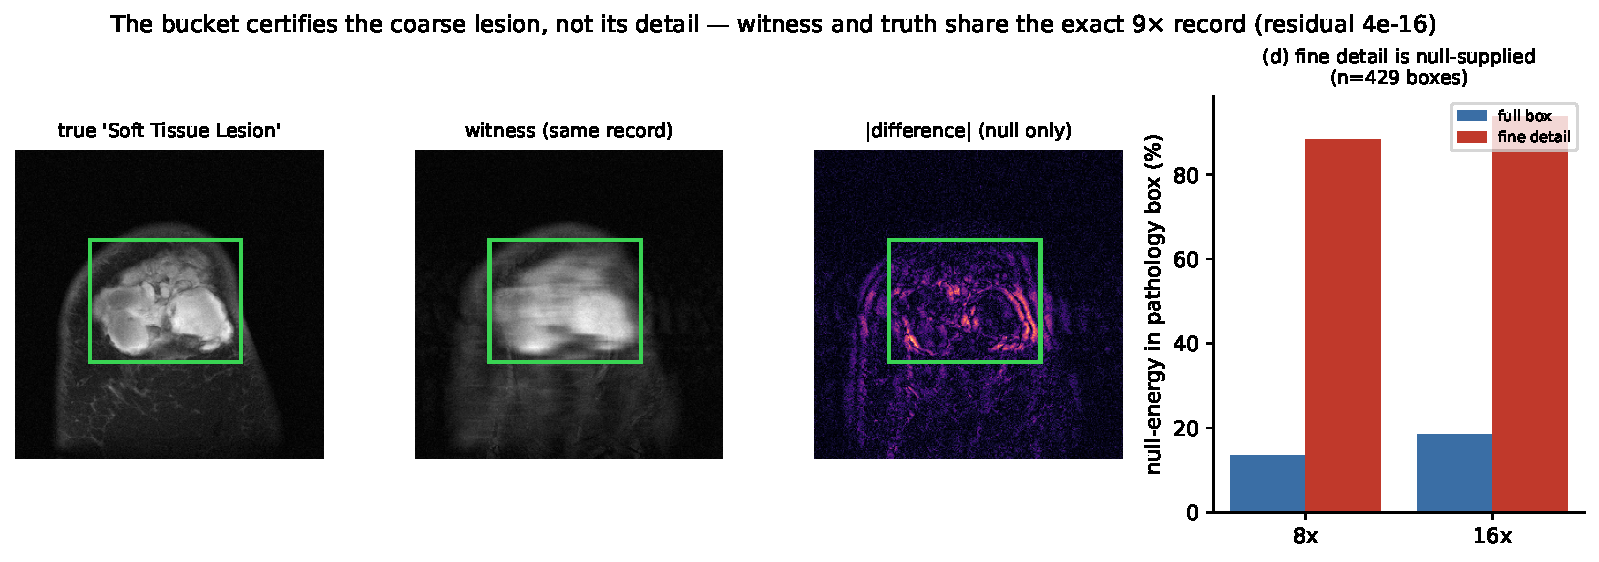
\includegraphics[width=1.0\linewidth]{DECISION_MRI.pdf}
\caption{\textbf{Coarse-certified, fine-detail-uncertified.} Across $429$ real fastMRI+ pathology boxes, the ACS certifies the coarse lesion (full-box null median $13.5\%$ at $R{=}8$) while its fine-detail contrast is $88.4\%$ null-supplied; a record-preserving null-space edit shifts fine contrast by $-43\%$ with $Ax=y$ held to $10^{-16}$.}
\end{figure}

\subsection*{E.3 CASSI: forensics over the MST model zoo}

The masked-Fourier operator hides the modal-contraction theorem behind a flat spectrum. Snapshot compressive spectral imaging exposes it. We ran the decomposition on SD-CASSI (shift-mask-sum, a $28$-band cube $\to$ a $256\times310$ snapshot, $23.1\times$ undersampling) using the \textbf{real released} TSA-Net gray coded aperture (fill $0.563$), over $13$ published models from the MST model zoo on that shared operator. Because $AA^\top = \operatorname{diag}(\Phi_s)$ is \textit{exactly} diagonal, $A^\dagger$, $P_R$, $P_0$ and the entire singular spectrum are closed-form, $O(N)$, with no SVD; the identities hold in float64 to $\sim\!10^{-13}$.

\textbf{The non-uniform spectrum is the empirical face of the modal-contraction theorem.} The measured singular values $\sigma_j = \sqrt{\Phi_s}$ over $79{,}360$ detector modes span $[0.009,\,4.907]$ (median $3.51$) --- a $528\times$ ratio. The per-mode audit contraction $\lambda/(\lambda+\sigma_j^2)$ at $\lambda=10^{-3}$ therefore spans $[4.15\times10^{-5},\,9.21\times10^{-1}]$, a $2\times10^{4}\times$ spread, where masked-Fourier MRI (E.2) collapses to the single value $9.99\times10^{-4}$. The theorem's mode-dependence is measured on a real coded aperture, not designed.

\textbf{Wiring validated against published PSNR.} Before attributing, we confirmed the operator wiring reproduces each model's published simulation PSNR (ours vs. reported): MST-S $34.38$ vs $34.26$; HDNet $35.06$ vs $34.97$; BIRNAT $37.73$ vs $37.58$; DAUHST-9stg $38.18$ vs $38.36$. The ledger below is computed on the same operator that reproduces the field's own numbers.

\textbf{Table E4. Attribution over the MST model zoo (shared real coded aperture, range ceiling $19.04$ dB).} \textit{Gain} is over the min-norm $A^\dagger y$ ceiling. \textit{Null share} is the fraction of that gain supplied from $\ker A$ (values slightly above $100\%$ mean the row-effect is negative --- the model's measured component is \textit{worse} than the ceiling). \textit{Drift} is $\lVert A\hat{x}-y\rVert/\lVert y\rVert$.

\begin{center}\begin{tabular}{lcccc}
\toprule
Model & PSNR (dB) & Gain over ceiling & Null share & Record drift \\
\midrule
TSA-Net & $31.67$ & $+12.63$ & $101\%$ & $5.3\%$ \\
GAP-Net & $29.57$ & $+10.52$ & $93\%$ & $11.9\%$ \\
DGSMP & $32.68$ & $+13.64$ & $101\%$ & $5.9\%$ \\
HDNet & $35.06$ & $+16.02$ & $101\%$ & $3.2\%$ \\
MST-S & $34.38$ & $+15.33$ & $101\%$ & $3.8\%$ \\
MST-M & $35.04$ & $+16.00$ & $101\%$ & $3.1\%$ \\
MST-L & $35.33$ & $+16.29$ & $101\%$ & $2.9\%$ \\
DAUHST-2stg & $35.31$ & $+16.27$ & $101\%$ & $2.8\%$ \\
CST-L & $35.94$ & $+16.90$ & $101\%$ & $2.6\%$ \\
MST++ & $36.10$ & $+17.06$ & $101\%$ & $2.6\%$ \\
BIRNAT & $37.73$ & $+18.69$ & $100\%$ & $1.3\%$ \\
$\lambda$-Net & $28.65$ & $+9.61$ & $101\%$ & $5.3\%$ \\
DAUHST-9stg & $38.18$ & $+19.14$ & $100\%$ & $0.9\%$ \\
\bottomrule
\end{tabular}\end{center}

The reading is near-uniform: twelve of the thirteen models supply $100$--$101\%$ of their PSNR gain over the $19.04$ dB ceiling from the null space, with the row-effect slightly \textbf{negative} --- the models mildly corrupt the measured component rather than repairing it. GAP-Net is the sole exception ($93\%$ null, a positive row-effect, and the largest drift, $11.9\%$). The entire decade of CASSI progress (TSA-Net $31.67\to$ DAUHST-9stg $38.18$, $+6.5$ dB of SOTA) happens \textit{entirely} in the null ledger, and the models are $0.9$--$12\%$ record-inconsistent throughout.

\textbf{The tautology defense, stated where it bites hardest.} At $m\ll n$ the null-dominance of a record-consistent estimator's error is definitional ($AP_0=0$ plus the orthogonal split), not a finding, and we do not present it as one (main §5, §6.3). What is \textit{contingent} --- not entailed by undersampling, and therefore the content --- is fourfold: (i) the measured record-inconsistency of the published models ($0.9$--$12\%$), which a data-consistent estimator would not have; (ii) the slightly \textit{negative} row-effect, models moving the measured component away from $A^\dagger y$; (iii) the specific $528\times$ non-uniform CASSI spectrum; and (iv) the cross-model agreement of the split over a whole zoo. The ledger is accounting, not accusation: the null content these models supply is largely truth-aligned. Its \textit{location} --- entirely in the uncertifiable ledger, on the field's own operator --- is the finding.

\medskip\hrule\medskip

\section*{Appendix F. Negative results}

\subsection*{F.1 Abandoned negative result: posterior $z$-sampling diversity}

We investigated whether stochastic $z$-sampling could turn the null-space prior into a calibrated posterior over $P_0 x$, and we report it only as a coverage limitation, not as a positive contribution. A deterministic checkpoint collapses: fixed-$y$ pixel std $\approx 10^{-3}$ and $P_0$ variance $1.09\times10^{-6}$ (gate 1). Removing the row-space reconstruction pressure lifts the collapse --- the anti-collapse diagnostic reaches $P_0$ variance $1.28\times10^{-3}$ (gate 2) --- confirming that the full reconstruction loss, not the architecture, was suppressing feasible null-space variation. But restored spread is not calibrated coverage. The best anchor/diversity scan still reaches only $\approx 45\%$ pixel and $\approx 48\%$ $P_0$ coverage at the nominal $90\%$ level, because the deterministic base estimate is offset from ground truth in the null space (base $P_0$ det-to-GT RMSE $\approx 0.081$): diversity can widen the sample cloud while leaving it centered in the wrong place. Sampling quality is therefore bounded by the base estimator's null-space accuracy, not only by the diversity mechanism. We make \textbf{no} posterior-diversity or calibrated-uncertainty claim; the line is retained solely to bound what the dial does and does not deliver.

The prior-content map in detail: on the $64\times64$ Rademacher validation, per-pixel $|P_0\hat{x}|$ and actual null-space error are essentially uncorrelated (Spearman $-0.079$, Pearson $-0.069$ for the LMMSE arm; $\approx 0.07$ for learned arms), and the top-10\% highest-magnitude pixels carry \textit{lower} error ($0.071$) than the rest ($0.079$). The map is provenance, not error.


\end{document}
